\documentclass[a4paper,twoside]{article}
\usepackage{vntex}
%\usepackage[english,vietnam]{babel}
%\usepackage[utf8]{inputenc}
\usepackage{lipsum}
\usepackage{setspace}
%\usepackage[utf8]{inputenc}
%\usepackage[francais]{babel}
\onehalfspacing % Set line spacing to 1.5

\usepackage{graphicx}
\graphicspath{ {./images/} }
\usepackage{float}
\usepackage{a4wide,amssymb,epsfig,latexsym,multicol,array,hhline,fancyhdr}
\usepackage{booktabs}
\usepackage{amsmath}
\usepackage{lastpage}
\usepackage[lined,boxed,commentsnumbered]{algorithm2e}
\usepackage{enumerate}
\usepackage{color}
\usepackage{graphicx}							% Standard graphics package
\usepackage{array}
\usepackage{tabularx, caption}
\usepackage{multirow}
\usepackage[framemethod=tikz]{mdframed}% For highlighting paragraph backgrounds
\usepackage{multicol}
\usepackage{rotating}
\usepackage{graphics}
\usepackage{geometry}
\usepackage{setspace}
\usepackage{epsfig}
\usepackage{tikz}
\usepackage{listings}
\usetikzlibrary{arrows,snakes,backgrounds}
\usepackage{hyperref}
\usepackage{scrextend}
\changefontsizes{13pt}
\usepackage{svg}
\hypersetup{urlcolor=blue,linkcolor=black,citecolor=black,colorlinks=true} 
%\usepackage{pstcol} 								% PSTricks with the standard color package

\newtheorem{theorem}{{\bf Định lý}}
\newtheorem{property}{{\bf Tính chất}}
\newtheorem{proposition}{{\bf Mệnh đề}}
\newtheorem{corollary}[proposition]{{\bf Hệ quả}}
\newtheorem{lemma}[proposition]{{\bf Bổ đề}}

\usepackage{adjustbox}

% \everymath{\color{blue}}
%\usepackage{fancyhdr}
\setlength{\headheight}{40pt}
\pagestyle{fancy}
\fancyhead{} % clear all header fields
\fancyhead[L]{
 \begin{tabular}{rl}
    \begin{picture}(25,15)(0,0)
    \put(0,-8){
\includegraphics[width=8mm, height=8mm]{Images/hcmut.png}}
    %\put(0,-8){
\epsfig{width=10mm,figure=hcmut.eps}}
   \end{picture}&
	%
\includegraphics[width=8mm, height=8mm]{hcmut.png} & %
	\begin{tabular}{l}
		\textbf{\bf \ttfamily Trường Đại Học Bách Khoa Tp.Hồ Chí Minh}\\
		\textbf{\bf \ttfamily Khoa Khoa Học và Kỹ Thuật Máy Tính}
	\end{tabular} 	
 \end{tabular}
}
\fancyhead[R]{
	\begin{tabular}{l}
		\tiny \bf \\
		\tiny \bf 
	\end{tabular}  }
\fancyfoot{} % clear all footer fields
\fancyfoot[L]{\scriptsize \ttfamily BTL2 môn Hệ cơ sở dữ liệu - HK241 Năm học 2024-2025}
\fancyfoot[R]{\scriptsize \ttfamily Trang {\thepage}/\pageref{LastPage}}
\renewcommand{\headrulewidth}{0.3pt}
\renewcommand{\footrulewidth}{0.3pt}


%%%
\setcounter{secnumdepth}{4}
\setcounter{tocdepth}{3}
\makeatletter
\newcounter {subsubsubsection}[subsubsection]
\renewcommand\thesubsubsubsection{\thesubsubsection .\@alph\c@subsubsubsection}
\newcommand\subsubsubsection{\@startsection{subsubsubsection}{4}{\z@}%
                                     {-3.25ex\@plus -1ex \@minus -.2ex}%
                                     {1.5ex \@plus .2ex}%
                                     {\normalfont\normalsize\bfseries}}
\newcommand*\l@subsubsubsection{\@dottedtocline{3}{10.0em}{4.1em}}
\newcommand*{\subsubsubsectionmark}[1]{}
\makeatother

\definecolor{dkgreen}{rgb}{0,0.6,0}
\definecolor{gray}{rgb}{0.5,0.5,0.5}
\definecolor{mauve}{rgb}{0.58,0,0.82}
\definecolor{backcolor}{RGB}{212,235,242}
\lstset{frame=tb,
	language=R,
	aboveskip=3mm,
	belowskip=3mm,
	showstringspaces=false,
	columns=flexible,
	basicstyle={\small\ttfamily},
	numbers=none,
	numberstyle=\tiny\color{gray},
	keywordstyle=\color{blue},
	commentstyle=\color{dkgreen},
	stringstyle=\color{mauve},
	breaklines=true,
	breakatwhitespace=true,
	tabsize=3,
	numbers=left,
	stepnumber=1,
	numbersep=1pt,    
	firstnumber=1,
	numberfirstline=true,
}

\definecolor{codegray}{gray}{0.9} % Define codegray here before use
\lstset{
    basicstyle=\ttfamily\footnotesize,   % Font style and size
    backgroundcolor=\color{codegray},     % Background color
    frame=single,                        % Single-line frame
    framerule=0.4pt,                     % Frame line thickness
    framesep=5pt,                        % Space between frame and code
    captionpos=b,                        % Caption position below the code
    breaklines=true,                     % Enable line breaking if code is too long
    numbers=left,                        % Line numbers on the left side
    numberstyle=\color{gray},       % Style of line numbers
    stepnumber=1,                        % Number lines every 1 line
    numbersep=5pt,                       % Space between line numbers and code
    tabsize=2,                           % Tab size
    showstringspaces=false,               % Do not replace spaces in strings with symbols
    language=sql,                      % Specify the code language
    keywordstyle=\color{blue},             % Keywords color
    commentstyle=\color{green!50!black},      % Comments color
    stringstyle=\color{red!50!black}          % String color
    %morekeywords={self,super} % Additional keywords, you may specify this line to highlight more keywords
}

\usepackage{indentfirst}
\begin{document}
\setlength{\parindent}{0.5cm}

\begin{titlepage}
\begin{center}
ĐẠI HỌC QUỐC GIA THÀNH PHỐ HỒ CHÍ MINH \\
TRƯỜNG ĐẠI HỌC BÁCH KHOA \\
KHOA KHOA HỌC - KỸ THUẬT MÁY TÍNH 
\end{center}

\begin{figure}[h!]
\begin{center}

\includegraphics[scale = 0.27]{Images/hcmut.png}
\end{center}
\end{figure}


\begin{center}
\begin{tabular}{c}
	\multicolumn{1}{l}{\textbf{{\Large HỌC KỲ 241}}}\\
	~~\\
	\hline
	\\
	\multicolumn{1}{l}{\textbf{{\Large Bài tập lớn}}}\\
	\\
	\textbf{{\Huge HỆ CƠ SỞ DỮ LIỆU }}\\
	\\
	\hline
\end{tabular}
\end{center}

\begin{table}[h]
\begin{tabular}{rrll}
\hspace{2.5 cm} & GVHD: &Nguyễn Thanh Tùng &\\
& Lớp: & CN02 & Nhóm 06 \\
% & Nhóm: & 06  &\\
& SV: & Nguyễn Lê Vân Tú& 2252881\\
& &   Huỳnh Minh Khoa& 2252346\\
& &Thân Nguyễn Minh Khoa & 2252361\\
& & Trần Lương Yến Nhi & 2252586\\
 & & \\
\end{tabular}
\end{table}
\begin{center}
{\footnotesize TP. HỒ CHÍ MINH, THÁNG 12/2024}
\end{center}
\end{titlepage}


\thispagestyle{empty}
\section*{Phân chia công việc}

% \begin{figure}[h!]
%     \centering
%     \hspace*{-1.5cm}
%     \includegraphics[width=1.2\linewidth]{Phan_cong.png}
%     % \caption{Enter Caption}
%     \label{fig:enter-label}
% \end{figure}

% \begin{figure}[h!]
%     \hspace*{-1.4cm}
%     \includegraphics[width=1.2\linewidth]{Phan_cong_.png}
%     % \caption{Enter Caption}
%     \label{fig:enter-label}
% \end{figure}

\newpage


\hspace*{-1cm}
% \begin{adjustbox}{lap=0cm}

% \setlength{\oddsidemargin}{-1cm} % Giảm lề trái 1cm
% \setlength{\evensidemargin}{-1cm}

\begin{table}[h]
    \centering
     % \hspace*{-1cm}

    
    \begin{tabular}{|p{1cm}|p{4cm}|p{1.5cm}|p{6cm}|p{1.5cm}|}
   
    \hline
    STT  & Name & Student ID & Task & Com- mitment\\ \hline
       1&Nguyễn Lê Vân Tú  & 2252881 & Packet Tracer/GNS3 simulation setup. Testing and validation (ping, traceroute, connectivity checks). Report writing and presentation preparation. & 25\%  \\ \hline 
       2& Huỳnh Minh Khoa & 2252346 & Main Site Network Design (Part 1): Requirements analysis for Main Site. Initial topology design for Buildings A and B, Data Center. VLAN planning for Main Site. & 25\%  \\ \hline
       3& Thân Nguyễn Minh Khoa &2252361  & Auxiliary Sites \& WAN: Requirements analysis for Auxiliary Sites. Topology design for Auxiliary Sites. WAN connection design (SD-WAN/MPLS, OSPF), 2xDSL with Load Balancing. & 25\%  \\ \hline 
       4& Trần Lương Yến Nhi  & 2252586 & Main Site Network Design (Part 2) \& Security: Wireless network design for Main Site. Security implementation plan (firewall, IPS/IDS, DMZ). VPN configuration.& 25\% \\ \hline
    \end{tabular}
    % \caption{Caption}
    \label{tab:my_label}
\end{table}   
% \end{adjustbox}

\newpage
\tableofcontents
\newpage

\section{Nội dung trong BTL 1}
\subsection{Context}
\textbf{PharmaCare} là một nền tảng được thiết kế để phục vụ người dùng có nhu cầu mua thuốc một cách tiện lợi, uy tín, an toàn và nhanh chóng. Cung cấp nền tảng để khách hàng có thể tìm kiếm, tham khảo thông tin, và mua các loại thuốc và sản phẩm y tế một cách dễ dàng và tiện lợi. Hỗ trợ người dùng tiếp cận với các sản phẩm uy tín, rõ nguồn gốc và đảm bảo chất lượng từ nhà cung cấp. Cung cấp thông tin hữu ích về dược phẩm, tư vấn sức khỏe và các dịch vụ liên quan đến chăm sóc sức khỏe cho người dùng.

Đội ngũ nhân viên uy tín, chất lượng, các nhân viên sẽ có các thuộc tính như ID (unique), mật khẩu, tài khoản, tên, địa chỉ, số điện thoại, có thuộc tính phức hợp lương hàng tháng gồm thuộc tính dẫn xuất tổng lương và tháng. Tất các nhân viên sẽ thuộc 1 trong 2 nhóm full-time và part-time và có thể là dược sĩ hoặc quản kho, ngoài ra 1 nhân viên có thể được quản lý bởi 1 nhân viên là quản lý, 1 người quản lý có thể quản lý nhiều nhân viên. Các nhân viên có thể có 1 thực thể phụ thuộc là đơn vị lương, mỗi đơn vị lương đều thuộc về 1 nhân viên, gồm lương theo giờ và lương tăng ca. 1 nhân viên có thể làm nhiều ca và 1 ca có thể có nhiều nhân viên, 1 ca làm có các thuộc tính là ID (unique), thời gian bắt đầu và kết thúc giờ làm, ngoài ra ở chức năng làm trong ca sẽ có thuộc tính kết hợp thời gian làm gồm có ngày làm, thời gian bắt đầu và kết thúc giờ làm. Nhân viên có thể bắt đầu sớm hơn hoặc trễ hơn ca làm hay kết thúc sớm hơn hoặc trễ hơn ca làm. 1 dược sĩ có thể kê nhiều đơn thuốc, các đơn thuốc kê cho 1 đơn hàng đều do 1 dược sĩ kê, ngoài ra đơn thuốc do dược sĩ kê sẽ có 1 thực thể phụ thuộc là lịch sử gồm các thuộc tính là số thứ tự là khóa 1 phần, nội dung bị sửa đổi, 1 dược sĩ ứng với 1 đơn thuốc thì có thể có nhiều lịch sử thay đổi, 1 dược sĩ ứng với 1 lịch sử thay đổi chỉ thuộc về 1  đơn thuốc, 1  lịch sử thay đổi ứng với 1 đơn thuốc chỉ do 1 dược sĩ thay đổi. Chức năng thay đổi này có thuộc tính là ngày để ghi nhận lại thời gian thay đổi. Các đơn thuốc chia làm 2 loại, do được sĩ kê hoặc bác sĩ kê, mỗi đơn thuốc sẽ ứng với một chi tiết của đơn hàng và có các thuộc tính ngày, ID (unique). Các đơn thuốc được kê bởi bác sĩ có thuộc tính đa trị là hình chụp đơn thuốc 1 dược sĩ có thể chuẩn bị cho nhiều đơn hàng, mỗi đơn hàng đều được chuẩn bị bởi nhiều dược sĩ.

Thực thể phiếu chi gồm các thuộc tính là ID (unique), ngày trả và số tiền, có 2 thực thể con là trả cho nhà kho và trả cho nhân viên, 1 nhân viên có thể trả cho nhiều phiếu chi cho nhân viên nếu người nhân viên trả này là quản lý. Thực thể trả cho nhà kho sẽ được dùng để chi trả cho các đơn nhập kho bởi quản lý dựa theo số tiền của đơn kho. Tổng chi là tổng các khoản tiền đã được , gồm các thuộc tính là ID (unique), có thuộc tính kết hợp là thời gian gồm các thuộc tính tháng và năm, cuối cùng là 1  thuộc tính dẫn xuất tổng số tiền (đây là tổng tất cả số tiền đã chi trong 1 tháng). Mỗi Tổng chi đều có nhiều phiếu chi, một phiếu chi có thể thuộc về 1 tổng chi. Mỗi đơn kho gồm các thuộc tính là ID (unique), ngày nhập kho và thuộc tính dẫn xuất tổng trị giá là tổng tiền hàng mà đơn đó đã nhập. 1 quản kho có thể tạo ra nhiều đơn kho, mỗi đơn kho đều được xử lý bởi 1 quản kho. Ngoài ra còn có thực thể lô hàng, gồm có các thuộc tính là ID (unique), số lượng, trị giá, ngày sản xuất, ngày hết hạn. Mỗi đơn kho có thể có nhiều lô và mỗi lô đều được nhập bởi 1 đơn kho, ngoài ra 1 đơn xuất khỏi kho bởi 1 đơn xuất kho, chức năng xuất kho có thuộc tính đa trị lý do vì có thể có nhiều lý do để bỏ lô này ra khỏi kho như hết hạn sử dụng.

Thực thể sản phẩm sẽ có các thuộc tính là ID (unique), tên, công dụng, điều kiện bảo quản/ lưu trữ, quốc gia xuất xứ, giá, hướng dẫn sử dụng, chứng nhận, cảnh báo, đối tượng sử dụng, công ty sản xuất, mô tả và thuộc tính dẫn xuất tổng số lượng từ các lô hàng, nhãn. Mỗi sản phẩn đều thuộc về nhiều lô và 1 lô có thể có 1 sản phẩm. 1 sản phẩm có thể là thiết bị y tế hoặc sản phẩm có thể tiêu thụ. Thiết bị y tế  gồm các thuộc tính là loại, chất liệu, kích thước, yêu cầu, bảo hành, vô trùng. Sản phẩm có thể tiêu thụ được gồm các thuộc tính là nguyên liệu, liều dùng, dạng liều dùng (viên, siro,..), kích thước mỗi phần (vỉ 10 viên, gói 30ml, lọ 150ml, ...). Sản phẩm có thể tiêu thụ được có thể là thuốc hoặc thực phẩm chức năng. Thuốc gồm các thuộc tính là tác dụng phụ, chỉ định, theo toa. Thực phẩm chức năng có thuộc tính là thông tin về chất gây dị ứng.

Thực thể báo cáo hàng tháng, gồm các thuộc tính là ID (unique), ngày, cùng với 2 thuộc tính dẫn xuất là doanh thu và lợi nhuận. 1 báo cáo có thể có nhiều đơn hàng nhiều thực thể tổng chi và nhiều đơn hàng.

Thực thể đơn hàng là những đơn hàng khách hàng đặt gồm các thuộc tính như ID (unique), ghi chú của khách hàng, địa điểm giao hàng và có thuộc tính dẫn xuất khoảng cách, được tính bằng khoảng cách từ kho đến địa điểm nhận hàng. Đối với chức năng trả lại hàng hoặc bị boom hàng, hàng được trả từ đơn về lại lô, 1 đơn hàng có thể được trả về cho nhiều lô, 1 lô có thể được trả hàng bởi nhiều đơn, để biết sản phẩm của đơn thuộc lô nào sẽ do dược sĩ kê đơn từ ban đầu.

Thực thể phiếu giảm giá, có các thuộc tính như ID (unique), điều kiện, số lượng tiền giảm, tên, có thuộc tính kết hợp là ngày có hiệu lực gồm 2 ngày bắt đầu bà ngày kết thúc. Mỗi phiếu giảm giá đều có thể là phiểu giảm giá thuộc hệ thống hoặc phiếu giảm giá được quy đổi, phiếu giảm giá được quy đổi có thuộc tính là số điểm mà khác hàng cần để có thể quy đổi ra phiếu giảm giá này. Ngoài ra phiếu giảm giá còn có thể là phiếu giảm giá sản phẩm, là phiếu giảm giá chỉ dành riêng cho 1 sản phẩm có thuộc tính là nhãn sản phẩm đó. 1 phiếu giảm giá có thể thuộc về nhiều sản phẩm, 1 sản phẩm có thể có nhiều phiếu giảm giá sản phẩm, được phân biệt bởi nhãn, nhãn phiếu giảm giá sản phẩm cần phải giống nhãn sản phẩm. Mỗi khách hàng ứng với 1 phiếu giảm giá đặt nhiều đơn hàng. Ngoài ra ở chức năng đặt đơn sẽ có 1 thuộc tính là ngày đặt hàng và mỗi đơn hàng đều thuộc chức năng này. 

Ngoài ra sẽ có thực thể công ty vận chuyển, gồm các thuộc tính như ID (unique), tên, số điện thoại, địa chỉ, giá vận chuyển (thuộc tính đa trị vì mỗi công ty sẽ có nhiều giá vận chuyển khác nhau). Ngoài ra, 1 công ty có thể có nhiều shipper và mỗi shipper đều thuộc về 1 công ty logistic, shipper có thuộc tính là ID (unique), tài khoản, mật khẩu, số điện thoại, tên, biển số xe. 1 shipper có thể nhận nhiều đơn hàng và 1 đơn hàng chỉ được nhận bởi 1 shipper, việc nhận đơn của shipper gồm các thuộc tính là ngày nhận, mã vận đơn và thuộc tính dẫn xuất giá tiền, đây là tiền ship được tính từ khoản cách cũng như giá vận chuyển từ công ty vận chuyển. Thực thể tình trạng đơn hàng gồm thuộc tính ID (unique), tên, đây là các trạng thái đơn hàng, mỗi đơn hàng đều gồm 1 trạng thái đơn hàng và 1 trạng thái đơn hàng có thể được ghi nhận trong nhiều đơn hàng. Mỗi đơn hàng có thể có nhiều cập nhật đơn hàng, thực thể cập nhật đơn hàng là thực thể yếu, bao gồm những thuộc tính là nội dung cập nhật, ngày là khóa 1  phần. Mỗi cập nhật đơn hàng đều có 1  trạng thái đơn hàng và 1 trạng thái đơn hàng có thể bao gồm trong nhiều cập nhật đơn hàng. Ngoài ra, 1 shipper có thể tạo ra nhiều cập nhật đơn hàng và mỗi cập nhật đơn hàng đều đươc tạo ra bởi 1 shipper. Đơn hàng còn có 1  thực thể phụ thuộc là chi tiết đơn hàng, mỗi chi tiết đơn hàng có thuộc tính là số thứ tự là khóa 1  phần, 1  đơn hàng có thể có nhiều chi tiết đơn hàng, và ứng với một chi tiết đơn hàng là 1 sản phẩm ứng với số lượng của nó và mỗi sản phẩm có thể nằm trong nhiều chi tiết đơn hàng.

Mỗi khách hàng sẽ có các thuộc tính như ID (unique), tên, địa chỉ, tài khoản, mật khẩu, số điện thoại, ngoài ra còn có thuộc tính dẫn xuất điểm thưởng từ đơn hàng mà khách hàng đã đặt. Mỗi khách hàng có thể đổi được nhiều phiếu giảm giá. Mỗi phiếu giảm giá có thể được đổi bởi nhiều khách hàng và ngược lại khách hàng có thể đổi được nhiều phiếu giảm giá. Ngoài ra ở chức năng đổi còn có 1  thuộc tính là số lượng để biết được số lượng phiếu giảm giá có thể được đổi. Mỗi khách hàng còn có thể nhận được nhiều phiếu giảm giá hệ thống, 1  phiếu giảm giá hệ thống có thể được nhận bởi nhiều khách hàng, và ở chức năng nhận cũng sẽ có thuộc tính số lượng để biết được ứng với phiếu giảm giá đó khách hàng sẽ được nhận bao nhiêu phiếu. Ngoài ra khách hàng sẽ có thêm một vài chức năng:

Chức năng hỏi, 1 khách hàng có thể hỏi nhiều dược sĩ, 1 dược sĩ có thể trả lười nhiều khách hàng, có thuộc tính đa trị là hỏi gồm các thuộc tính là câu hỏi, câu trả lời, ngày. 

Chức năng đánh giá, 1 khách hàng có thể đánh giá nhiều sản phẩm, 1 sản phẩm có thể được đánh giá bới nhiều khách hàng. Có thuộc tính phức hợp là đánh giá gồm các thuộc tính là ngày, bình luận, xếp hạng (từ 0-5).

Có ràng buộc ngữ nghĩa mà không thể biểu diễn được là chỉ có nhân viên làm quản lý mới có thể trả lương cho nhân viên. Ngoài ra còn có trả hóa đơn nhà kho, mỗi hóa đơn kho có thể được trả 1 lần bởi phiếu chi cho kho. Doanh thu sẽ bằng tổng tiền tất cả các đơn hàng cộng lại. Lợi nhuận được tính bằng cách lấy doanh thu trừ cho tổng chi. Dược sĩ sẽ biết được lô mà sản phẩm thuộc về ngay từ lúc kê đơn do ID sản phẩm sẽ truy được lô của sản phẩm. Nếu shipper làm mất hàng thì công ty logistic sẽ là bên bồi thường. Ngoài ra để đổi voucher, thì tổng điểm thưởng cần lớn hơn hoặc bằng điểm cần đổi. Đối với các voucher sản phẩm thì giữa sản phẩm và voucher cần phải chung tag. Ngoài ra điểm đánh giá cho từng sản phẩm là từ 0 đến 5.
\newpage
\subsection{EERD}
Dưới đây là biểu đồ:
\begin{figure}[H]
 \hspace*{-2cm}
        \includesvg[width=1.2\columnwidth]{Images/EERD.svg}
         \caption{EERD}
\end{figure}
\subsection{Mapping}
Dưới đây là biểu đồ:
\begin{figure}[H]
\hspace*{-1.5cm}
        \includesvg[width=1.3\columnwidth]{Images/mapping.svg}
        \caption{Mapping}
\end{figure}

\newpage
\section{Tạo Cơ sở dữ liệu}
\subsection{Tạo bảng}
\textbf{Yêu cầu:}
Viết các câu lệnh hiện thực các bảng dữ liệu đã thiết kế. Sinh viên phải tự xác định kiểu dữ liệu, kích thước dữ liệu và các ràng buộc (dựa trên mô tả nghiệp vụ và EERD ở Assignment 1). Các loại ràng buộc tối thiểu cần có:
\begin{itemize}
\item Khoá chính có dạng số nguyên tăng dần. Ví dụ: 1, 2, 3…
\item Khoá chính có dạng [PREFIX][Số tăng dần có X ký số]. Ví dụ EMP00001, EMP00002,…
\item Ràng buộc duy nhất 
\item Ràng buộc khoá ngoại
\item Ràng buộc not null 
\item Ràng buộc kiểm tra miền trị liên quan đến một cột hoặc nhiều cột. Ví dụ, mã phòng ban nằm trong khoảng [0, 20], thời gian check in phải nhỏ hơn thời gian check out,…
\end{itemize}

\textbf{Hiện thực}
\begin{lstlisting}[language=SQL, caption=Tạo bảng Product] 
CREATE TABLE `batch_product`.`product` (
  `ID` int NOT NULL AUTO_INCREMENT,
  `Name` varchar(16) NOT NULL,
  `Description` varchar(1024) NOT NULL,
  `Origin` varchar(32) NOT NULL,
  `Tag` varchar(16) DEFAULT 'OTHER',
  `Storage_Condition` varchar(1024) DEFAULT NULL,
  `Country of origin` varchar(16) DEFAULT NULL,
  `Price` decimal(10,2) NOT NULL,
  `Directions for use` varchar(1024) NOT NULL,
  `Certificate` varchar(512) DEFAULT NULL,
  `Warning` varchar(512) DEFAULT NULL,
  `Intended User` varchar(128) DEFAULT NULL,
  `Total amount from batch` int DEFAULT '0',
  PRIMARY KEY (`ID`),
  UNIQUE KEY `Name` (`Name`),
  CONSTRAINT `product_chk_1` CHECK ((`Total amount from batch` >= 0))
)
\end{lstlisting}

\begin{lstlisting}[language=SQL, caption=Tạo bảng Employee] 
CREATE TABLE `employee` (
  `ID` int NOT NULL AUTO_INCREMENT,
  `Name` varchar(16) NOT NULL,
  `Address` varchar(64) DEFAULT NULL,
  `Account` varchar(32) DEFAULT NULL,
  `Password` varchar(16) DEFAULT NULL,
  `Phone_no` varchar(16) DEFAULT NULL,
  `WorkingType` varchar(64) DEFAULT NULL,
  `JobType` enum('pharmacist','inventory manager','product manager','admin') DEFAULT NULL,
  `Credential` varchar(128) DEFAULT NULL,
  PRIMARY KEY (`ID`),
  UNIQUE KEY `ID_UNIQUE` (`ID`),
  UNIQUE KEY `Phone_no_UNIQUE` (`Phone_no`)
)
\end{lstlisting}
\subsection{Insert vào bảng}

\begin{lstlisting}[language=SQL, caption= Thêm data vào table product] 
INSERT INTO `batch_product`.`product` (
    `Name`, 
    `Description`, 
    `Origin`, 
    `Tag`, 
    `Storage_Condition`, 
    `Country of origin`, 
    `Price`, 
    `Directions for use`, 
    `Certificate`, 
    `Warning`, 
    `Intended User`, 
    `Total amount from batch`
)
VALUES
('Vitamin D', 
 'Vitamin D supplements the immune system.', 
 'USA', 
 'VITAMIN', 
 'Store in a dry place, away from direct sunlight.', 
 'United States', 
 15.99, 
 'Take 1 tablet/day after meal.', 
 'FDA Approved', 
 'Not for use by persons under 6 years of age.', 
 'Adult', 
 100);
\end{lstlisting}

\begin{lstlisting}[language=SQL, caption= Thêm data vào table employee] 
 INSERT INTO `employee_prescription`.`employee` (
    `Name`, 
    `Address`, 
    `Account`, 
    `Password`, 
    `Phone_no`, 
    `WorkingType`, 
    `JobType`, 
    `Credential`
)
VALUES
('John Doe', 
 '123 Main St, New York, NY', 
 'johndoe123', 
 'pass1234', 
 '1234567890', 
 'Full-time', 
 'pharmacist', 
 'Pharmacist License A12345');
\end{lstlisting}



\subsection{Auto-export Script}
Ta dùng phần mềm MySQL Workbench để thực hiện lấy script của tất cả cấu trúc bảng, data, procedure, trigger.

Trong MySQL Workbench, sau khi kết nối với database cần export, ta chọn Server > Data Export
\begin{figure}[h!]
    \centering
    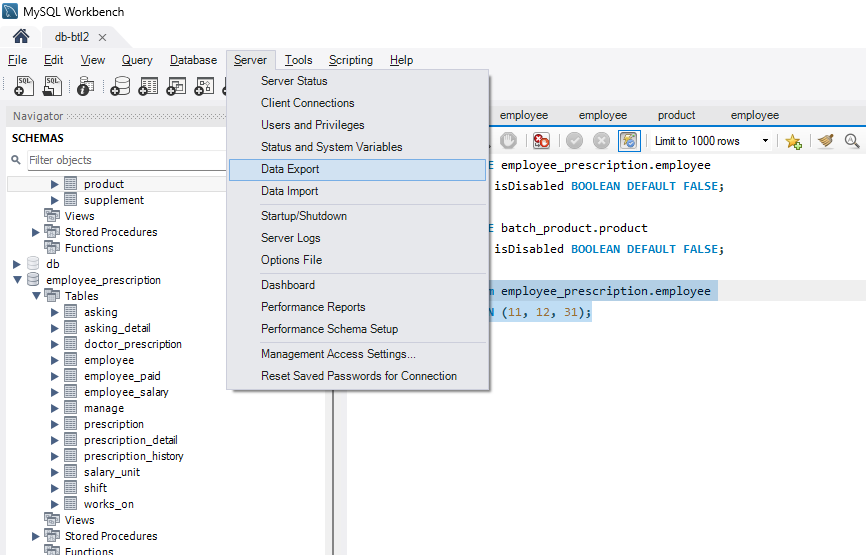
\includegraphics[scale=0.4]{Images/1.png}
    \caption{Chọn Data Export}
    % \label{fig:enter-label}
\end{figure}

Ta có một số các lựa chọn:
\begin{itemize}
    \item Tables to Export: Chọn các schema mà ta muốn export
    \item Objects to Export: Chọn có xuất các Procedures và Functions; Events; hoặc Triggers
    \item Export Options: Chọn xuất ra nhiều file hoặc một file, vị trí xuất file, ...
\end{itemize}
Sau khi tùy chọn xong, ta bấm Start Export
\begin{figure}[h!]
    \centering
    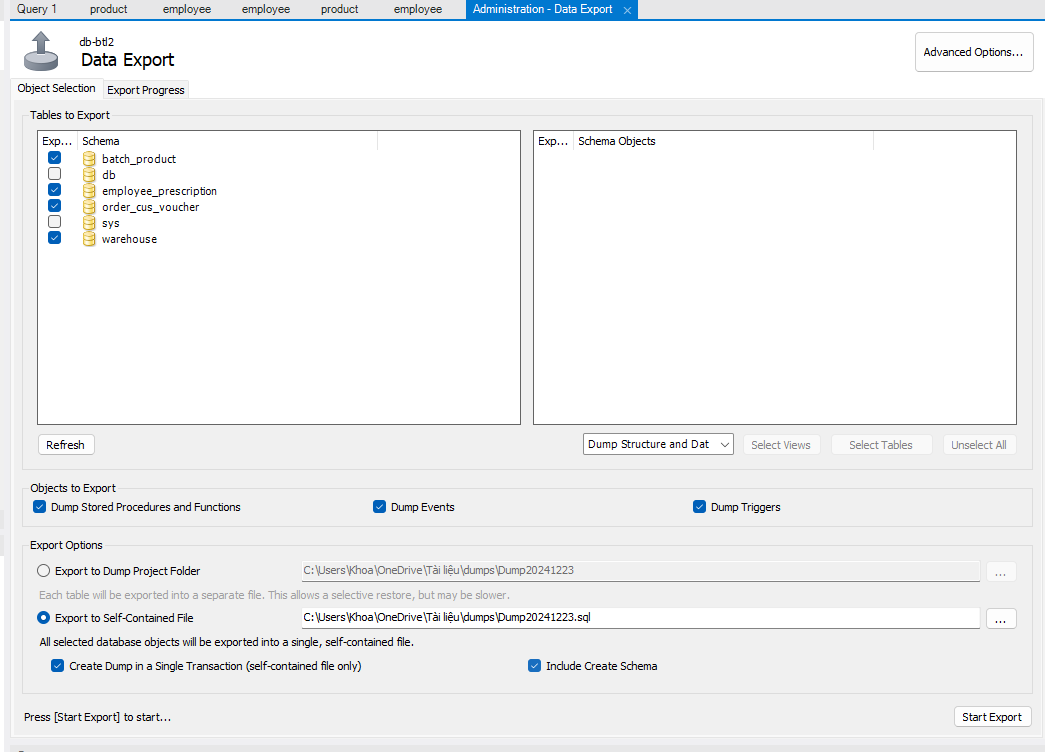
\includegraphics[scale=0.4]{Images/2.png}
    \caption{Màn hình chọn các tùy chọn để export}
    % \label{fig:enter-label}
\end{figure}

\newpage
Sau khi nhấn Start Export, ta sẽ được điều hướng đến màn hình này:
\begin{figure}[H]
    \centering
    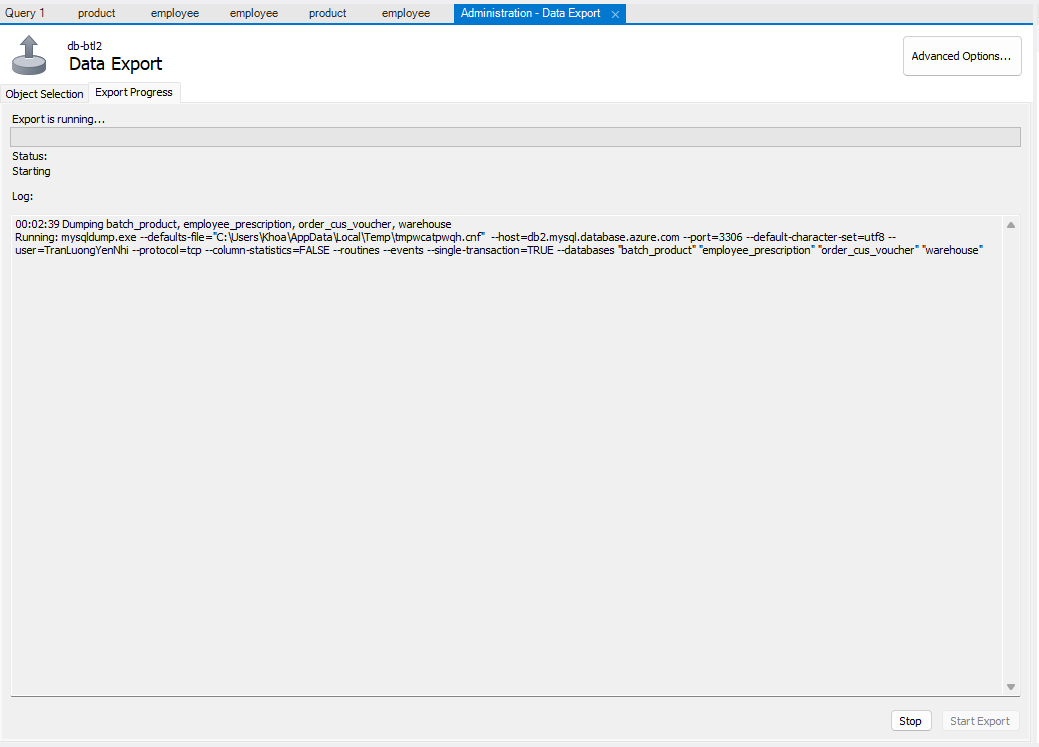
\includegraphics[scale=0.3]{Images/3.png}
    \caption{Màn hình trạng thái export}
    % \label{fig:enter-label}
\end{figure}


Đây là màn hình đó sau khi xong
\begin{figure}[H]
    \centering
    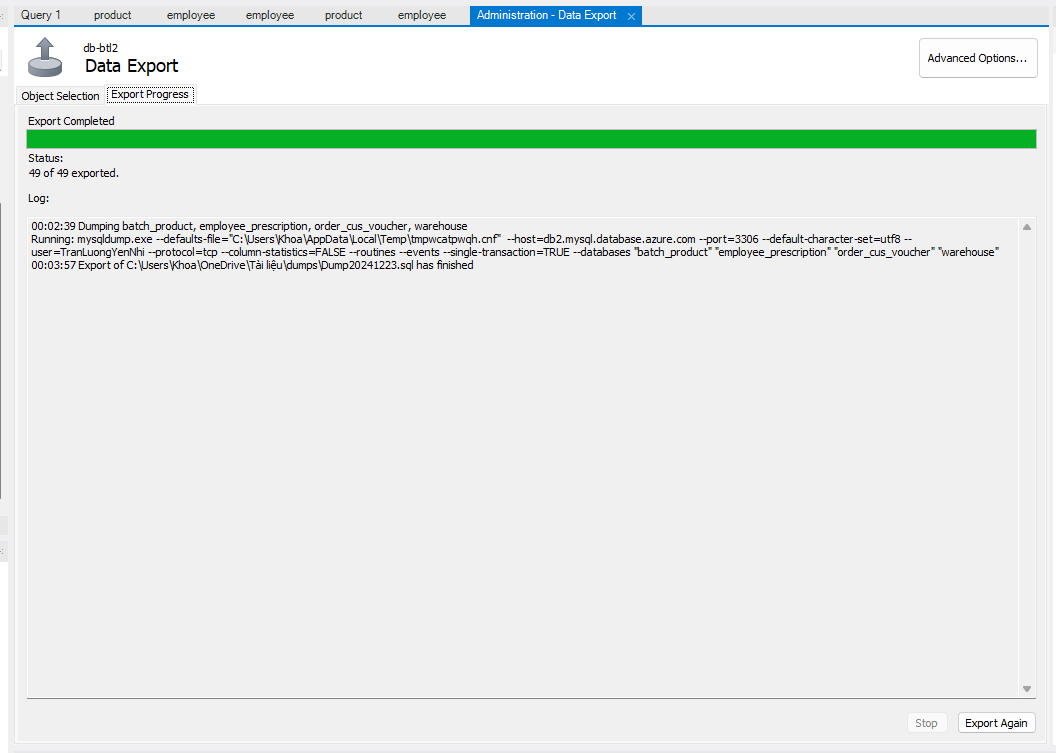
\includegraphics[scale=0.3]{Images/4.png}
    \caption{Màn hình hoàn thành export}
    % \label{fig:enter-label}
\end{figure}


%Set default listings style
\lstset{
    basicstyle=\ttfamily\footnotesize,  % Font style and size
    backgroundcolor=\color{codegray},   % Background color
    frame=single,                       % Single-line frame
    framerule=0.4pt,                    % Frame line thickness
    framesep=5pt,                       % Space between frame and code
    captionpos=b,                       % Caption position below the code
    breaklines=true,                    % Enable line breaking if code is too long
    numbers=left,                       % Line numbers on the left side
    numberstyle=\color{gray},      % Style of line numbers
    stepnumber=1,                       % Number lines every 1 line
    numbersep=5pt,                      % Space between line numbers and code
    tabsize=2,                          % Tab size
    showstringspaces=false,            % Do not replace spaces in strings with symbols
}


\section{STORE PROCEDURE/ FUNCTION/ TRIGGER}
\subsection{Store Procedure/ Function}
Trong database bao gồm nhiều procedure, một trong những procedure:\\
GetProductList Proceduce dùng để lấy thông tin của tất cả sản phẩm.

\begin{lstlisting}[language=SQL, caption=GetProductList Procedure] 
CREATE DEFINER=`TranLuongYenNhi`@`%` PROCEDURE `GetProductList`()
BEGIN
    SELECT
        p.ID,
        p.Name,
        p.Description,
        p.Origin,
        p.Tag,
        p.Storage_Condition,
        p.`Country of origin`,
        p.Price,
        p.`Directions for use`,
        p.Certificate,
        p.Warning,
        p.`Intended User`,
        p.`Total amount from batch`,
        c.Ingredient,
        c.Serving_size,
        c.Dosage,
        c.Dosage_form,
        c.Constraindication,
        m.Side_effect,
        m.Indication,
        m.Is_Prescription_Medicine,
        s.Allergen_info,
        me.Usage_Instruction,
        me.Material,
        me.`Size/Dimension`,
        me.Requirement,
        me.Warranty,
        me.Sterility,
        CASE
            WHEN me.ID IS NOT NULL THEN 'medical_equipment'
            WHEN m.ID IS NOT NULL THEN 'medicine'
            WHEN s.ID IS NOT NULL THEN 'supplement'
            WHEN c.ID IS NOT NULL THEN 'consumable'
            ELSE 'product'  
        END AS ProductType
    FROM
        product p
    LEFT JOIN
        consumable c ON p.ID = c.ID
    LEFT JOIN
        medicine m ON c.ID = m.ID
    LEFT JOIN
        supplement s ON c.ID = s.ID
    LEFT JOIN
        medical_equipment me ON p.ID = me.ID
    ORDER BY
        p.ID;
END ;;

\end{lstlisting}

\subsection{Trigger}

% \begin{figure}[H]
%  % \hspace*{-2cm}
%  \centering
%        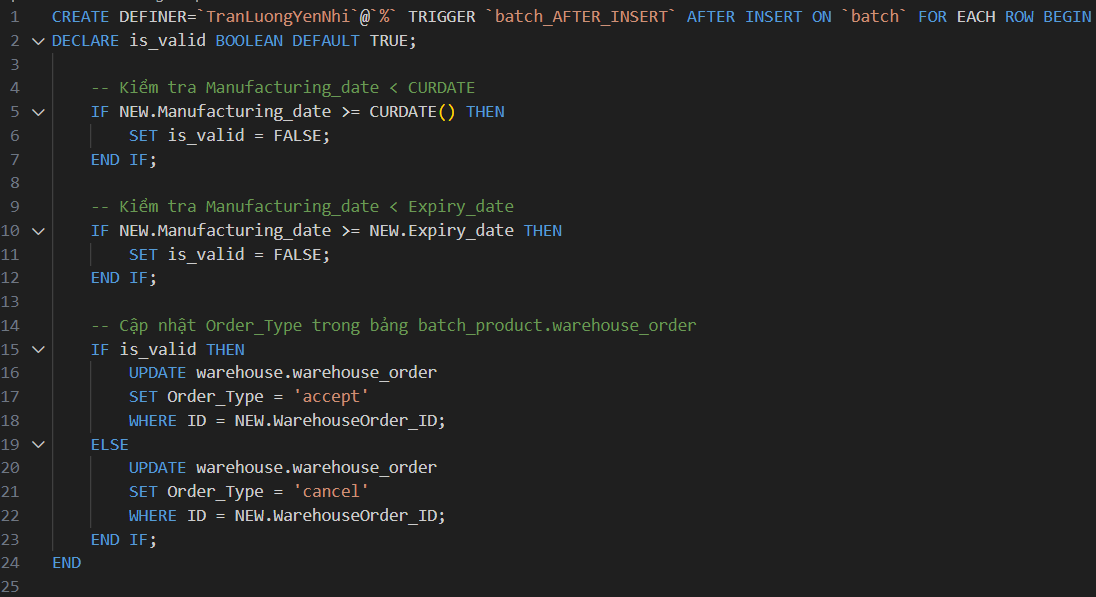
\includegraphics[width=1\linewidth]{trigger.png}
%        \caption{Trigger Batch}
% \end{figure}
\begin{lstlisting}[language=SQL, caption=Tạo trigger cho table Batch] 
CREATE DEFINER=`TranLuongYenNhi`@`%` TRIGGER `batch_AFTER_INSERT` AFTER INSERT ON `batch` FOR EACH ROW BEGIN
DECLARE is_valid BOOLEAN DEFAULT TRUE;

    IF NEW.Manufacturing_date >= CURDATE() THEN
        SET is_valid = FALSE;
    END IF;

    IF NEW.Manufacturing_date >= NEW.Expiry_date THEN
        SET is_valid = FALSE;
    END IF;

    batch_product.warehouse_order
    IF is_valid THEN
        UPDATE warehouse.warehouse_order
        SET Order_Type = 'accept'
        WHERE ID = NEW.WarehouseOrder_ID;
    ELSE
        UPDATE warehouse.warehouse_order
        SET Order_Type = 'cancel'
        WHERE ID = NEW.WarehouseOrder_ID;
    END IF;
END


\end{lstlisting}
Trigger này sẽ kiểm tra xem ngày sản xuất của lô hàng được thêm vào sẽ luôn sớm hơn hoặc bằng ngày hiện tại (thời điểm nhập lô) và hạn sử dụng, sau đó cập nhật trang thái vào đơn kho. Trigger này nhằm để từ chối các lô có thông tin sai lệch (do nhập sai hoặc hàng giả), đảm bảo tính hợp lý của thông tin lô hàng. 
\section{Tạo User và Xây dựng ứng dụng}
\subsection{Kiến trúc hệ thống}
\subsubsection{Database:}
\subsubsubsection{Kiến trúc:}
\begin{itemize}
    \item Thực hiện trên mySQL workbench.
    \item Được deploy trên Azure.
    \item Các câu truy vấn sẽ được gọi thông qua các Procedure hoặc Function nhằm đảm bảo bảo mật, không để lộ các thông tin truy vấn ra ngoài. Bên cạnh đó cũng sẽ giúp cải thiện Performance khi thực hiện truy vấn. 
    \item File code SQL đã được đính kèm trong bài nộp (Có thể chạy liền mạch từ đầu đến cuối code).
\end{itemize}
\subsubsubsection{Cách thực hiện:}
49 bảng sẽ được phân thành 4 schema khác nhau ứng với từng chức năng riêng biệt: batch\_product, employee\_prescription, order\_cus\_voucher, warehouse. Qua đó có thể dễ dàng quản lý các bảng và phân chia cho nhiều thành viên thực hiện. 
\subsubsection{Backend:}
\subsubsubsection{Kiến trúc:}
\begin{itemize}
    \item Ngôn ngữ: Javascript
    \item 2 Server: gRPC server và RestServer. Frontend sẽ truy cập vào endpoint được tạo trong RestServer, và thông qua đó RestServer sẽ gọi đến gRPC Server. Như vậy dữ liệu cũng sẽ được đảm bảo hơn. 
\end{itemize}
\subsubsection{Frontend:}
\subsubsubsection{Kiến trúc:}
\begin{itemize}
    \item Ngôn ngữ: TypeScript
    \item Gồm các lớp: entities (khai báo cấu trúc thực thể), service (đảm nhiệm vai trò kết nối với backend), hooks và các component.
    \item Hệ thống cũng sẽ thực hiện theo mô hình MVC, tách biệt các page thực hiện chức năng và trang giao diện người dùng. 
    \item Phối hợp giữa việc lưu local cho 1 session và lưu trên server để có thể tối ưu performance của hệ thống.
\end{itemize}




\subsection{Các luồng chức năng}
Hệ thống sẽ gồm 4 nhóm người dùng cính.
\begin{itemize}
    \item Admin: Đây sẽ là người dùng có thể thực hiện mọi chức năng và thông tin. Chỉ có admin là người tạo tài khoản cho nhân viên và nhân viên sẽ dùng các tài khoản đó để đăng nhập vào.
    \item Người quản lý sản phẩm: chỉ có thể xem được trang các sản phẩm và thêm, sửa hoặc xóa các sản phẩm. 
    \item Người quản lý kho: sẽ có thể xem được trang các sản phẩm và chọn các sản phẩm này để thêm vào đơn kho
    \item Nhân viên bán thuốc: sẽ là người xem được các sảm phẩm và từ các sản phẩm này sẽ tạo đơn thuốc cho khách hàng.
\end{itemize}
Ngoài ra, đối với các đơn kho khi nhập vào sẽ được kiểm tra hạn sử dụng, có còn nhập nữa không,... Bên cạnh đó, các đơn kho, đơn hàng cũng sẽ không được chỉnh sửa bởi bất kỳ ai để có thể minh bạch. 
Đối với các sản phẩm, người quản lý sản phẩm cũng có thể điều chỉnh xem sản phẩm này còn nhập nữa không hoặc Admin có thể xóa tài khoản nhân viên này không.
\section{Tự đánh giá}
\subsection{Điểm mạnh}
Hệ thống được thực hiện bài bản tại Database, Backend và Frontend cùng với các kiến trúc MVC, Multi Server. Qua đó, giúp cho hệ thống được thực hiện sát nhất với thực tế và đúng quy trình phần mềm. Ngoài ra hệ thống cũng được phân chia thành các lớp riêng biệt, đảm bảo mỗi phần là một chức năng qua đó giúp cho hệ thống dễ dàng bảo trì hoặc thay đổi.
\subsection{Điểm yếu}
Vì hệ thống được triển khai phức tạp, đòi hỏi phải tìm hiểu kĩ cũng như thực hiện nhiều công nghệ mới dẫn đến nghiệp vụ của hệ thống vẫn còn đơn giản. Bên cạnh đó, kiến thức vẫn còn hạn chế về nhiều mặt như giao diện nên giao diện người dùng vẫn chưa đẹp mắt và trải nghiệm tốt.
\section{Web "Quản lý nhà thuốc"}
\textbf{Đầu tiên, các server cần được bật lên:}
\begin{figure}[H]
\hspace*{1cm}     
    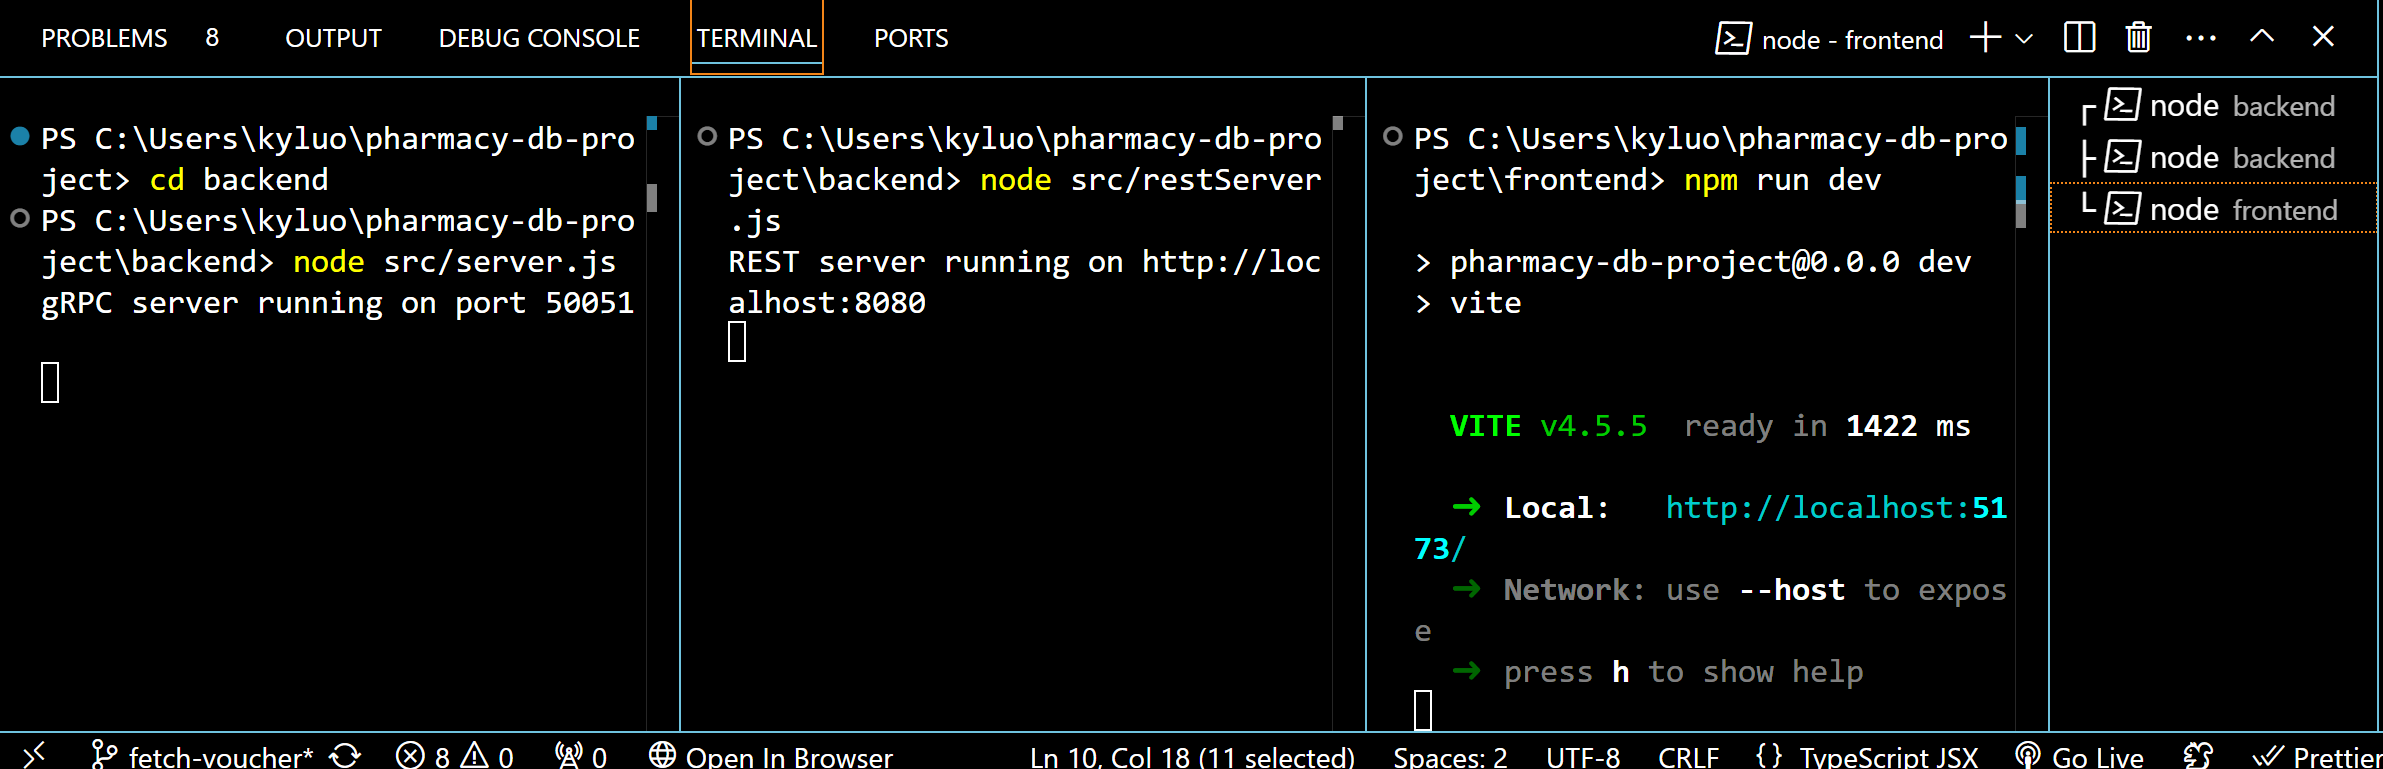
\includegraphics[scale=0.35]{Images/Screenshot 2024-12-23 152956.png}
\end{figure}
\textbf{Trang chủ của hệ thống khi chưa đăng nhập:}
   \begin{figure}[H]
        \hspace*{1cm}     
            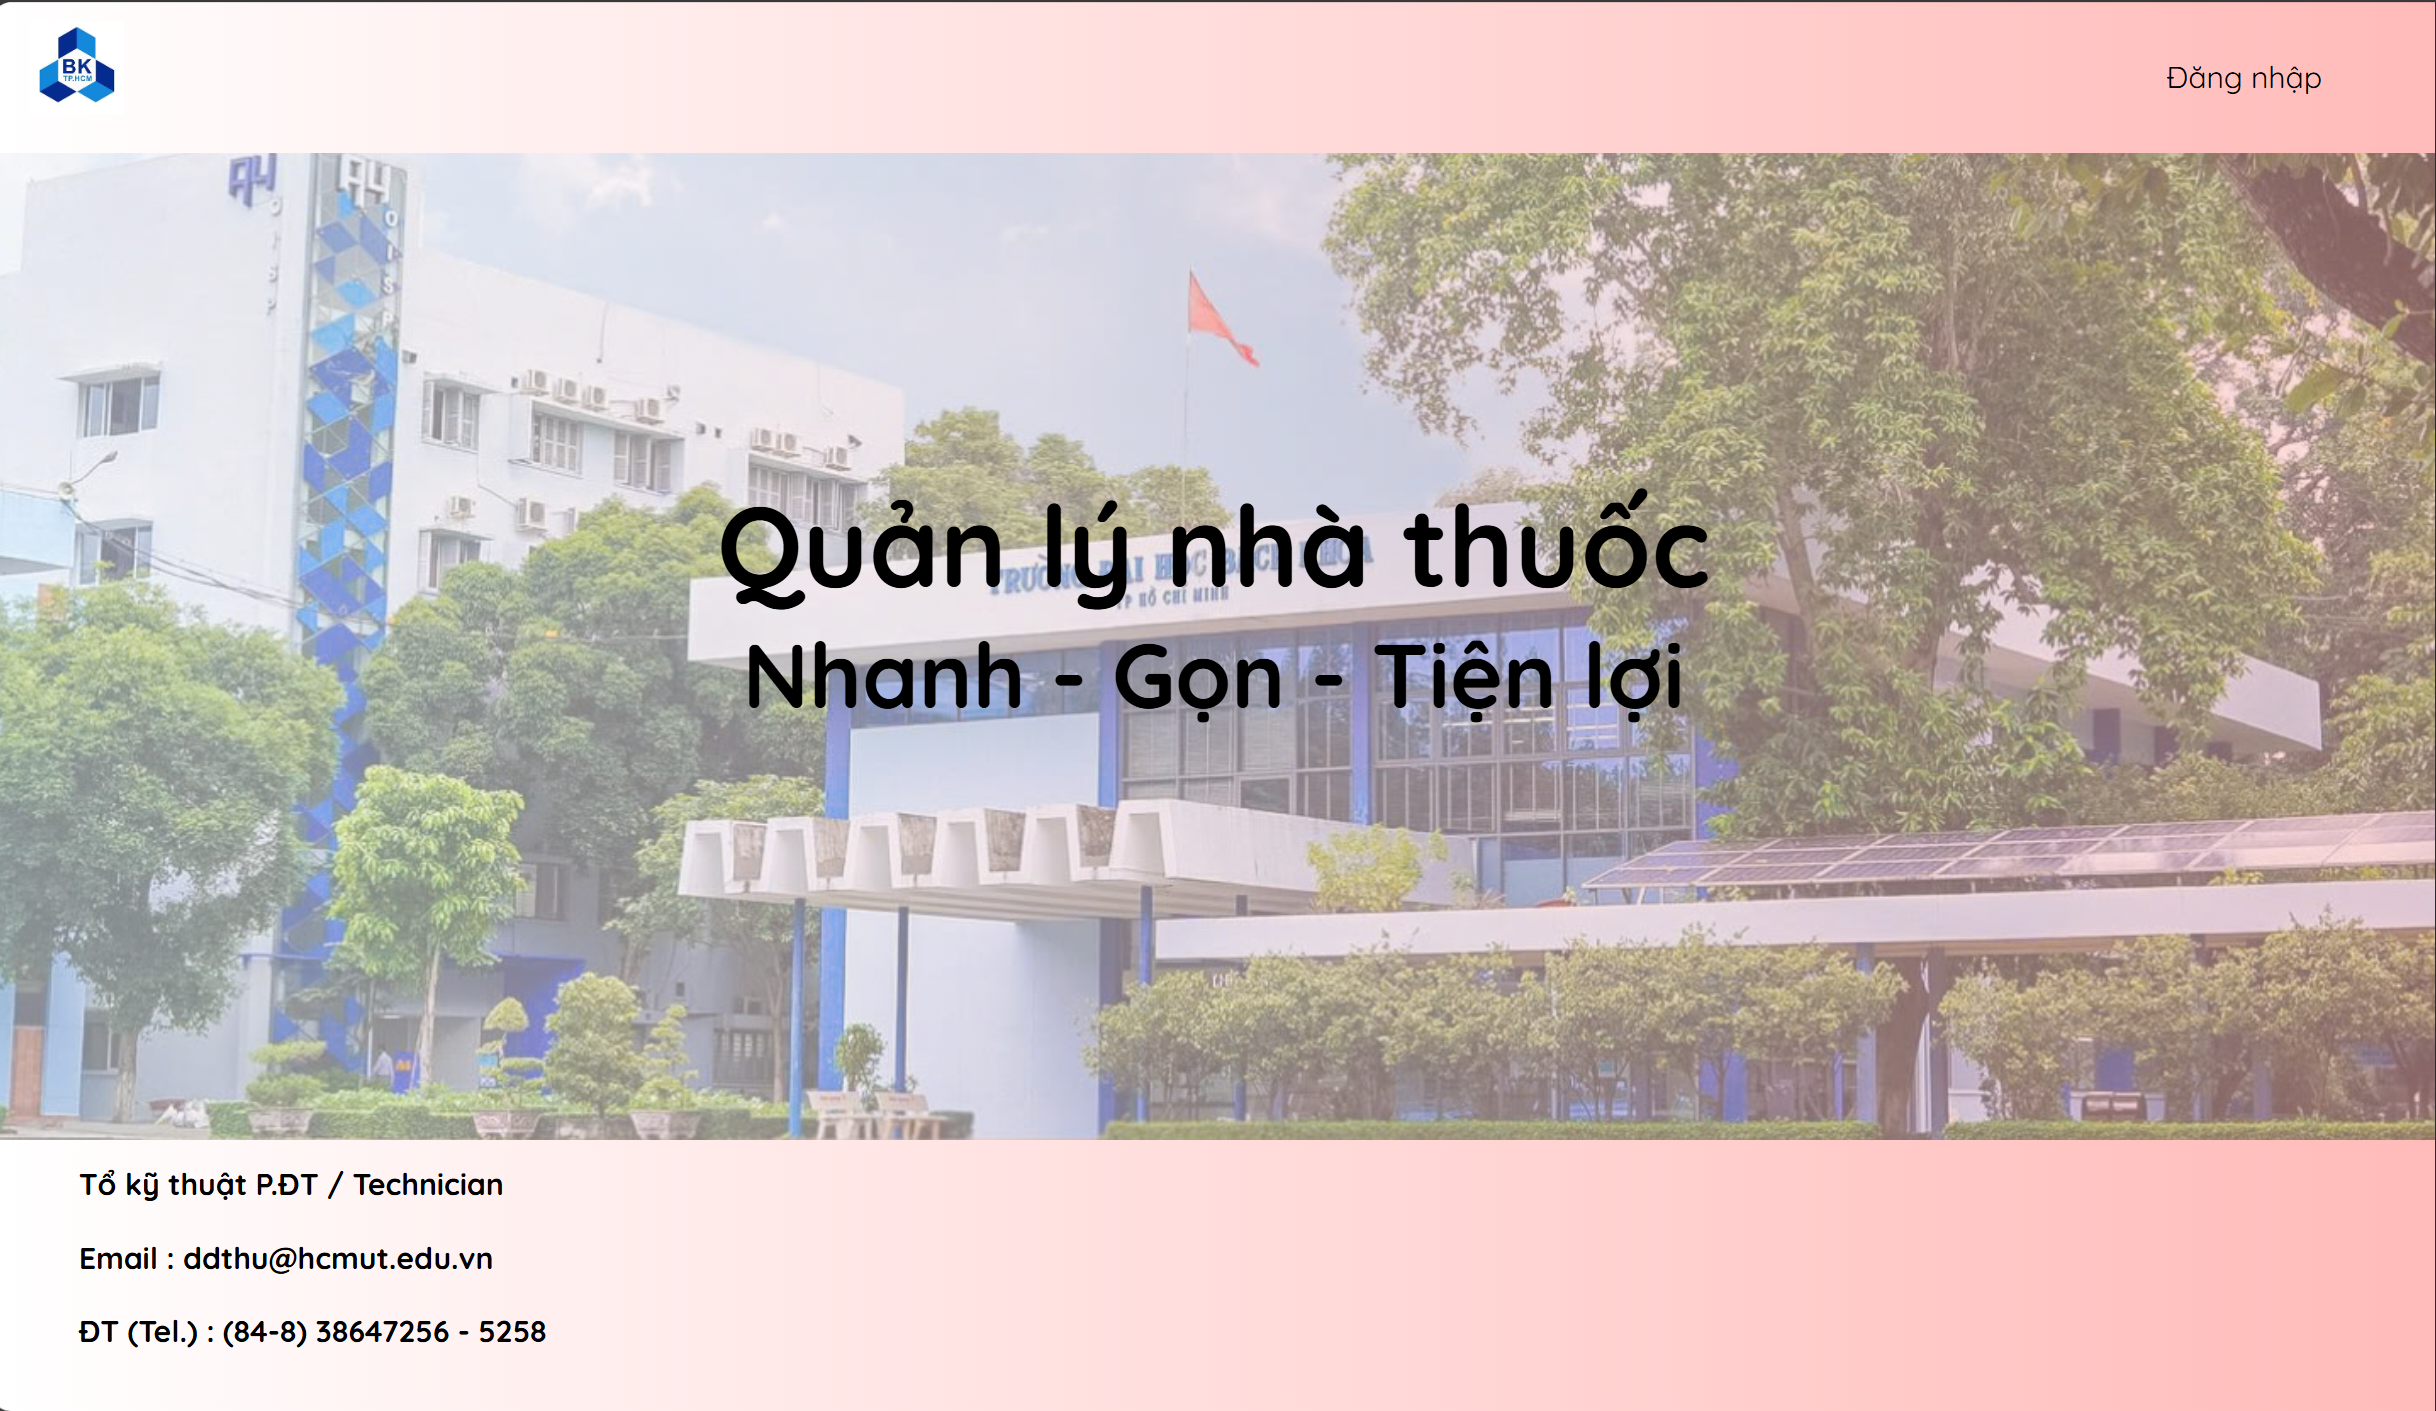
\includegraphics[scale=0.3]{Images/dnhap.png}
        \end{figure}

      \begin{figure}[H]
        \hspace*{1cm}     
            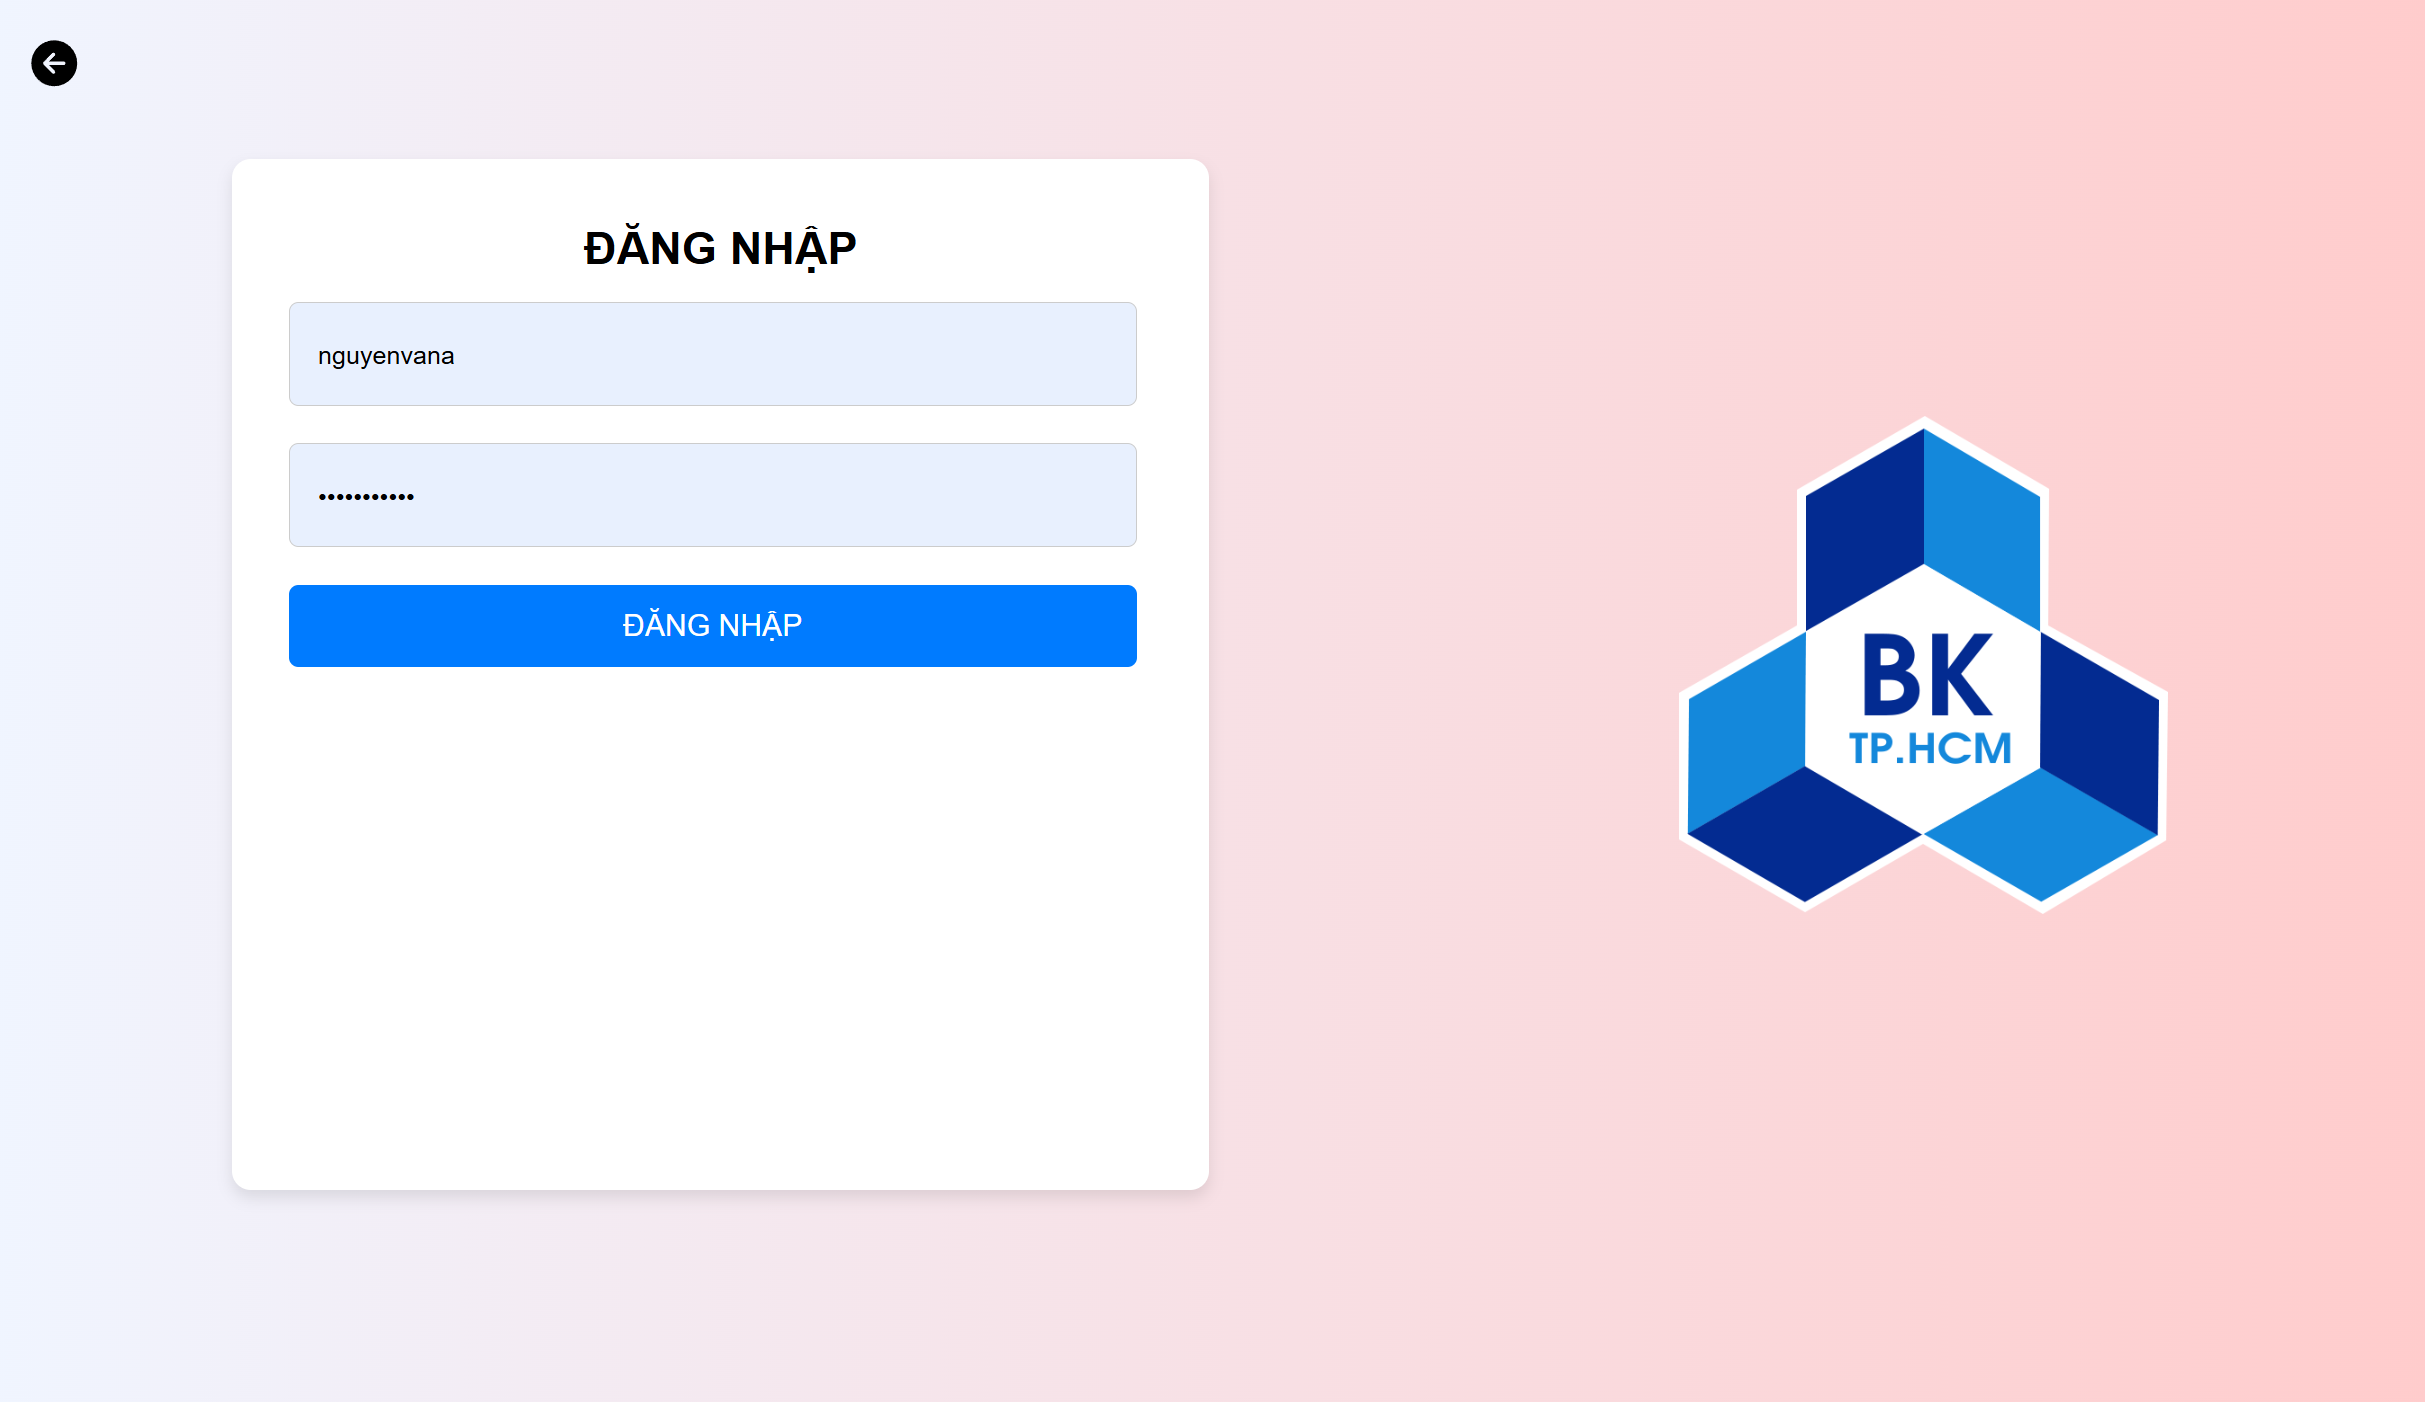
\includegraphics[scale=0.3]{Images/signin.png}
        \end{figure}
Hệ thống dành cho 4 người dùng chủ yếu ứng với các thanh menu riêng biệt:
\begin{itemize}
      \item \textbf{Admin (Người quản lý): }
        \begin{figure}[H]
        \hspace*{1cm}     
            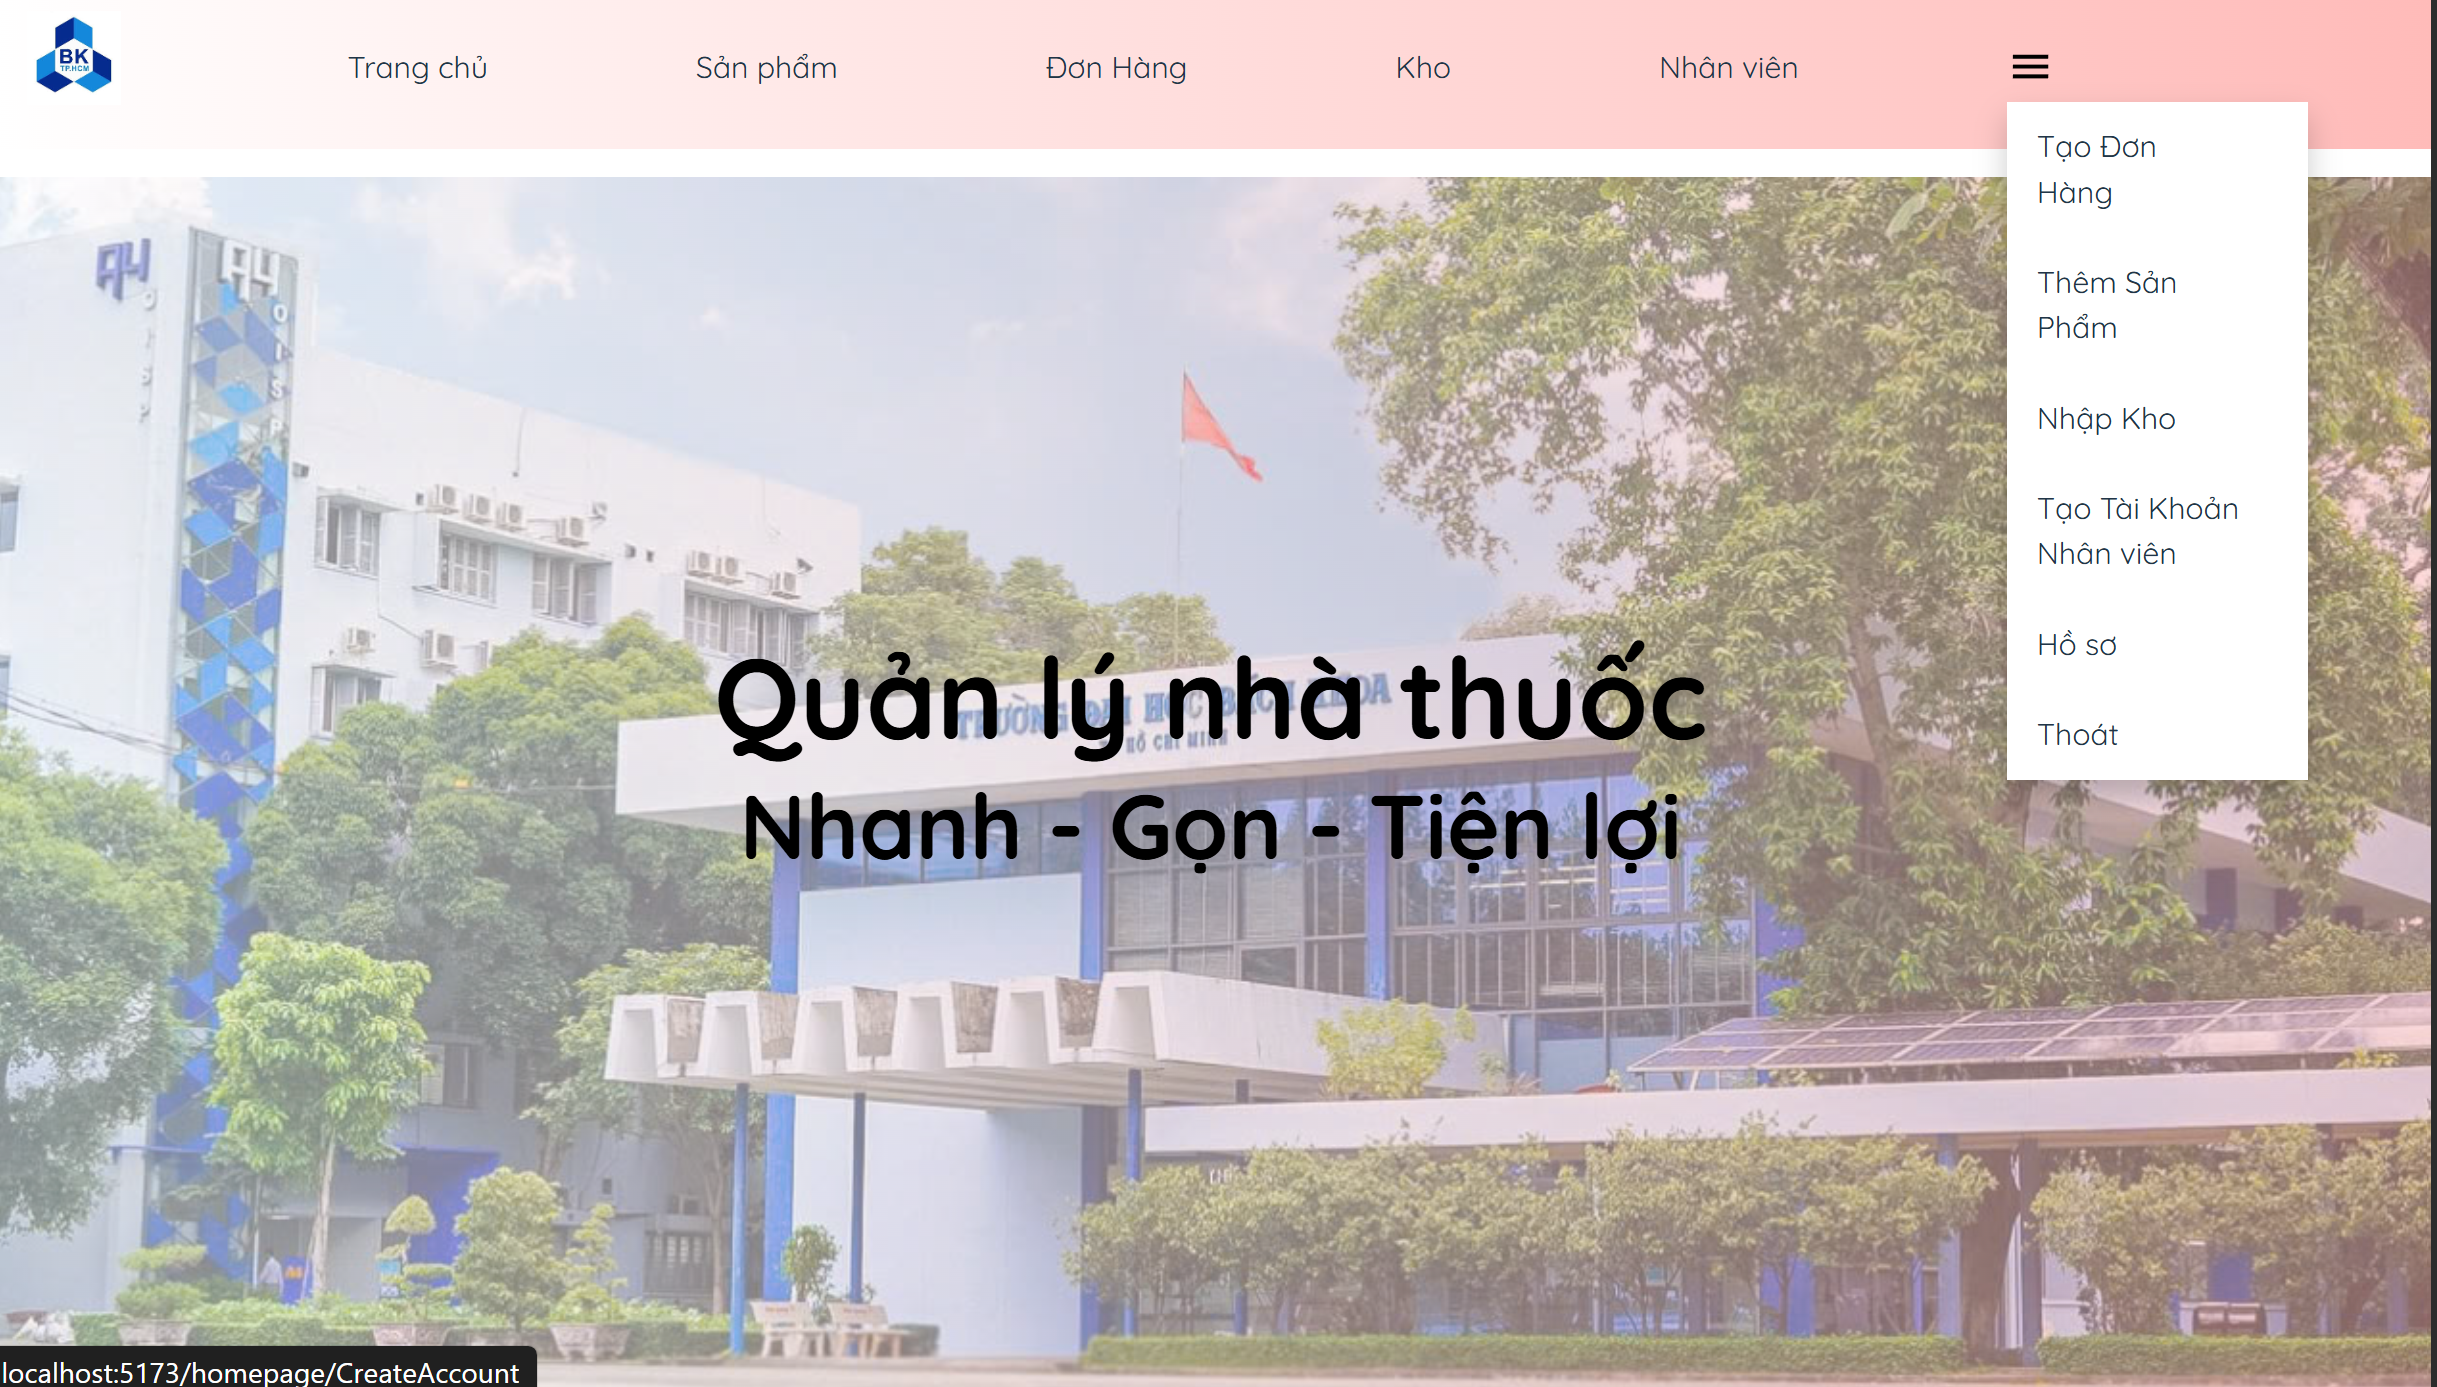
\includegraphics[scale=0.3]{Images/hp2.png}
        \end{figure}
        
      \item \textbf{Người quản lý sản phẩm: }
        \begin{figure}[H]
        \hspace*{1cm}     
            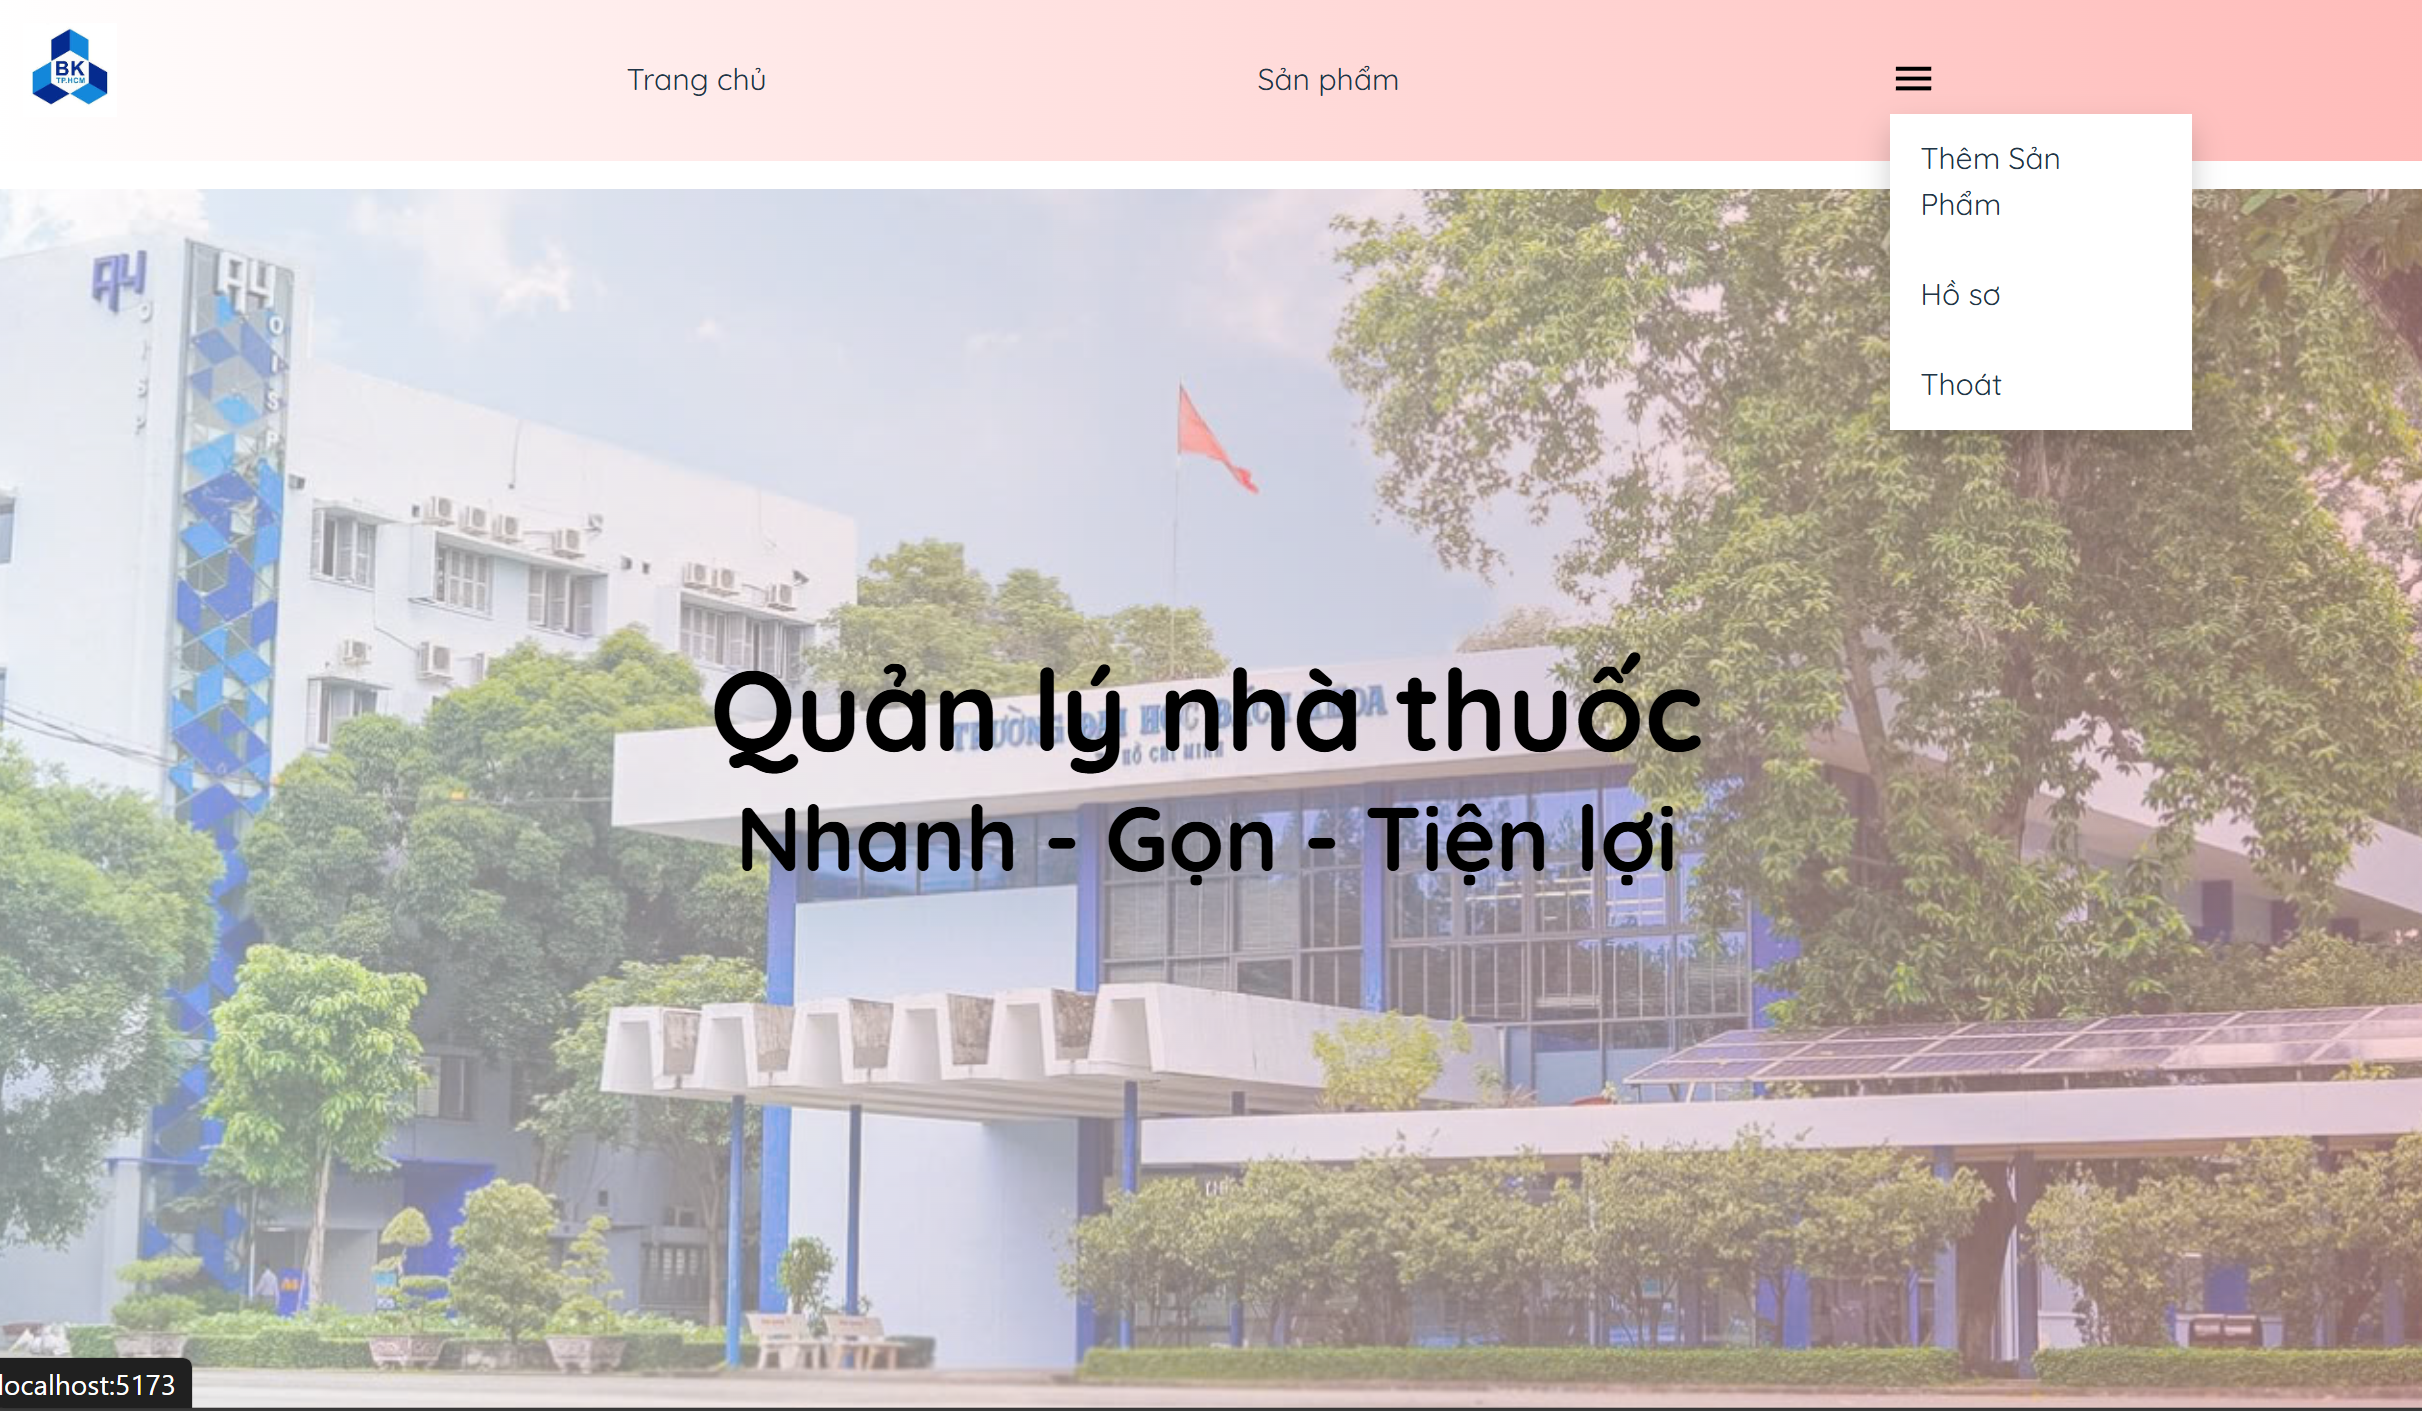
\includegraphics[scale=0.3]{Images/hp_prod.png}
        \end{figure}
        
      \item \textbf{Người quản kho: }
        \begin{figure}[H]
        \hspace*{1cm}     
            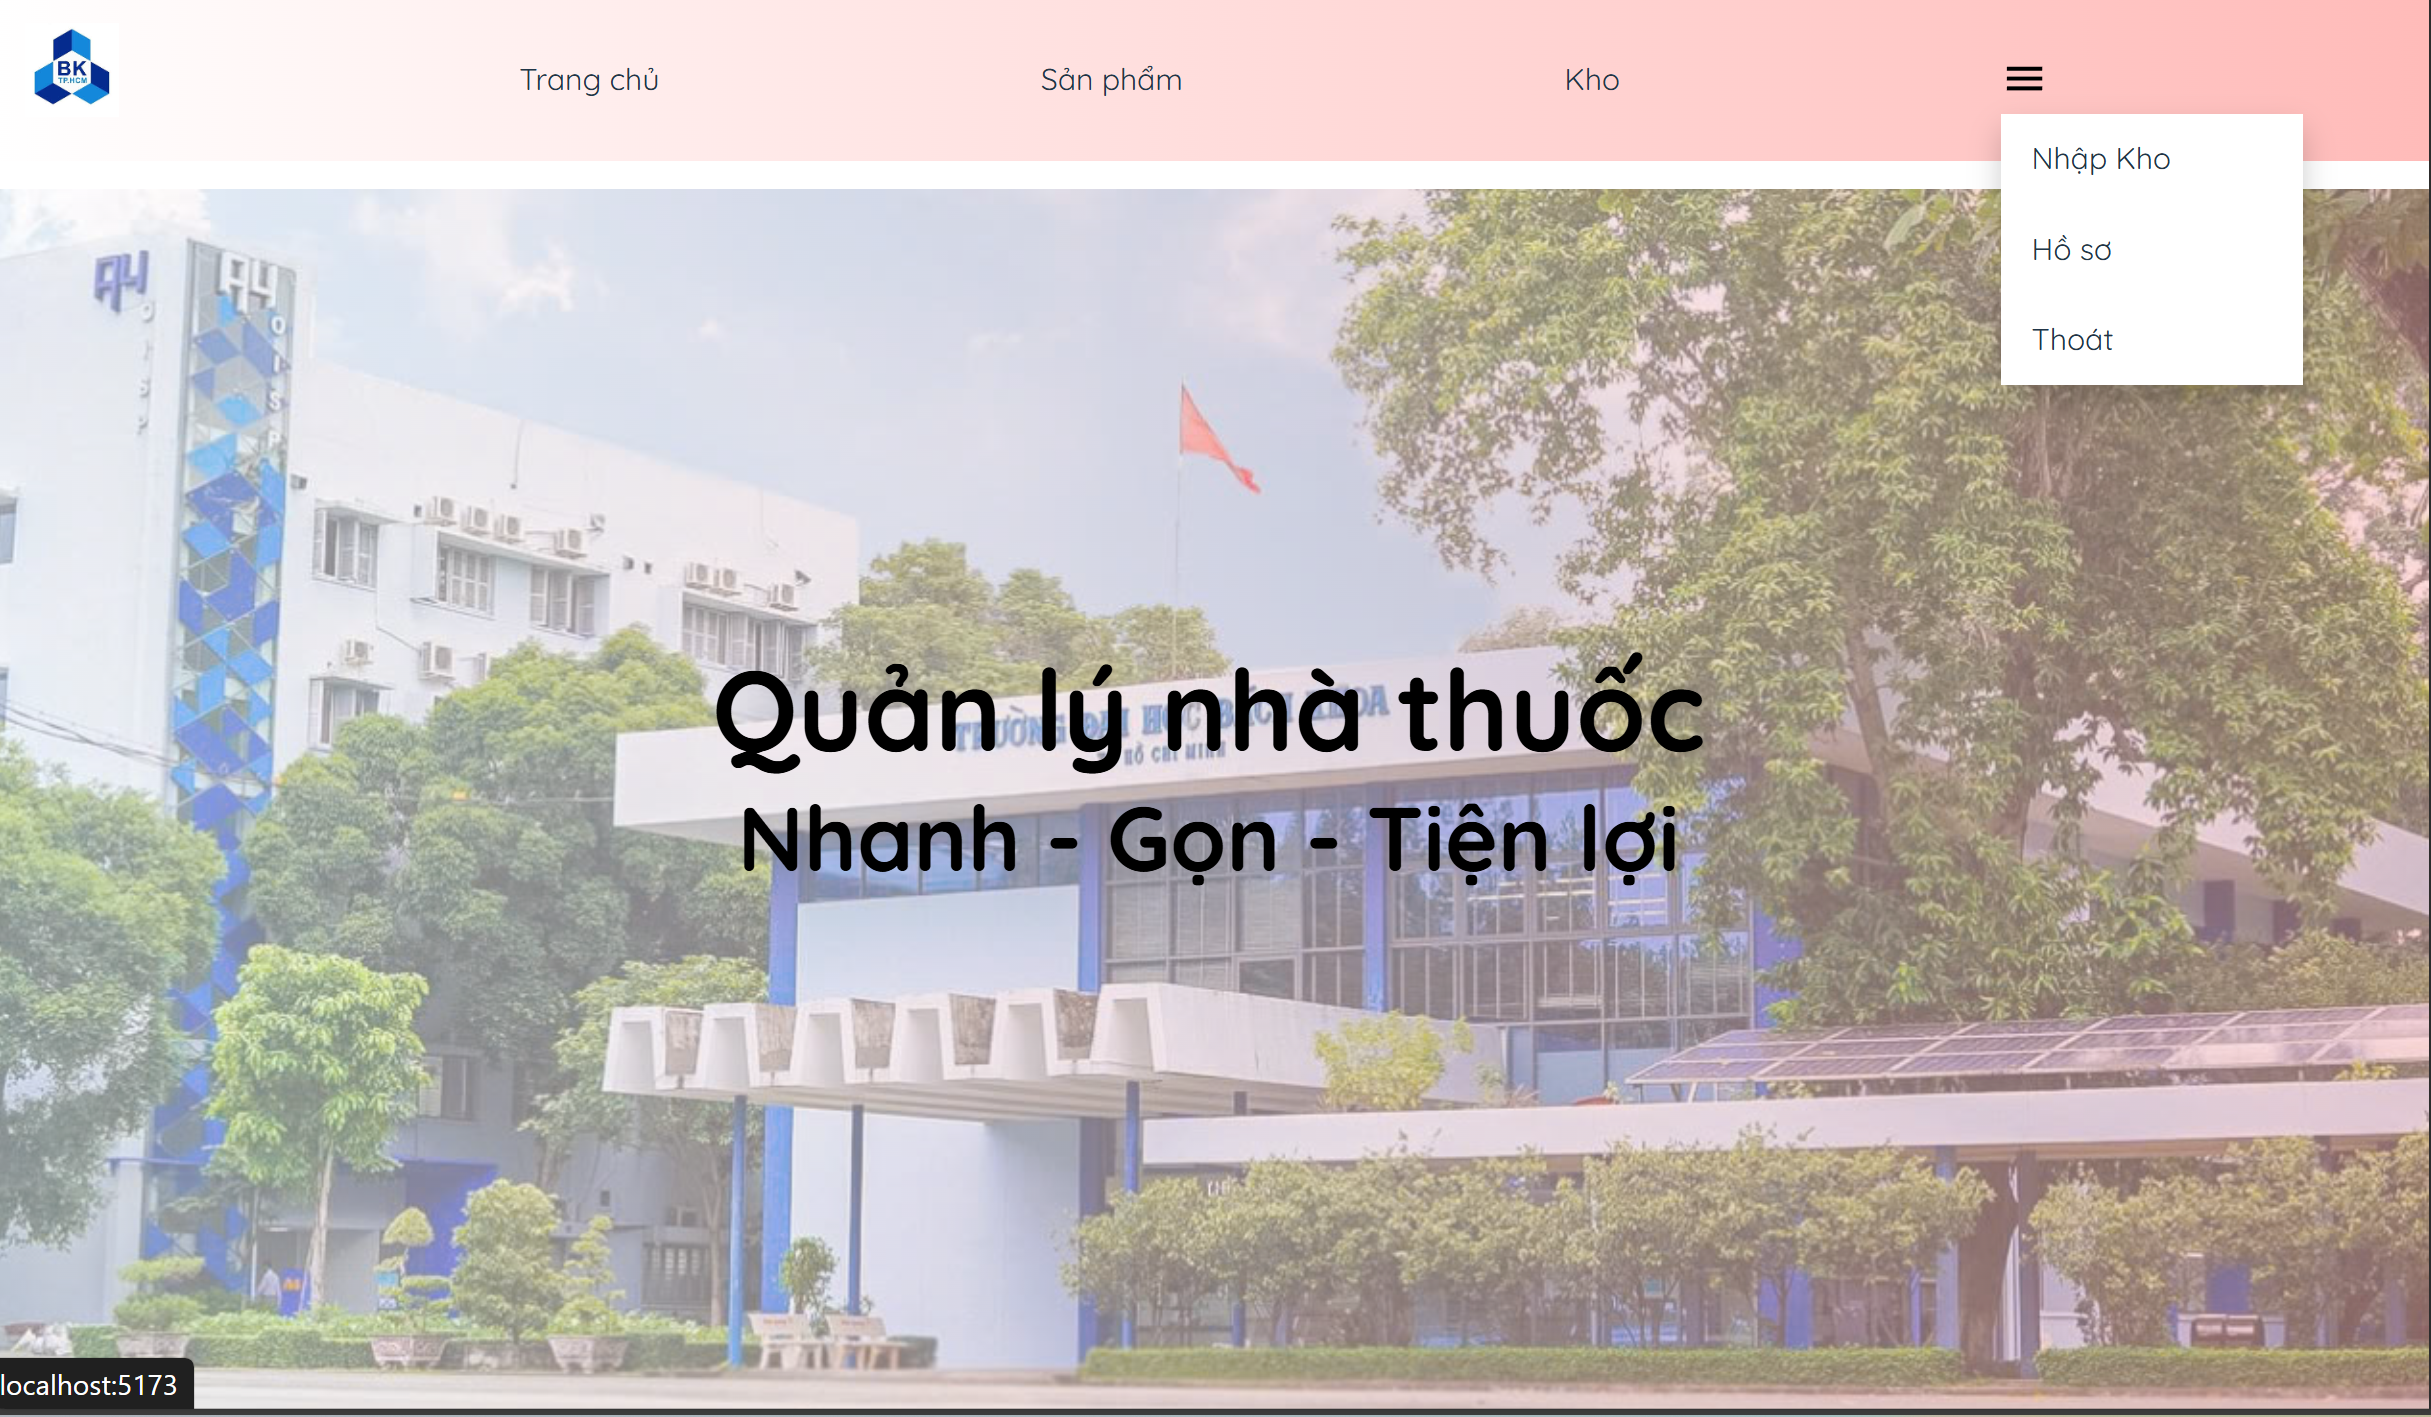
\includegraphics[scale=0.3]{Images/hp_inven.png}
        \end{figure}

     \item \textbf{Nhân viên bán thuốc: }
        \begin{figure}[H]
        \hspace*{1cm}     
            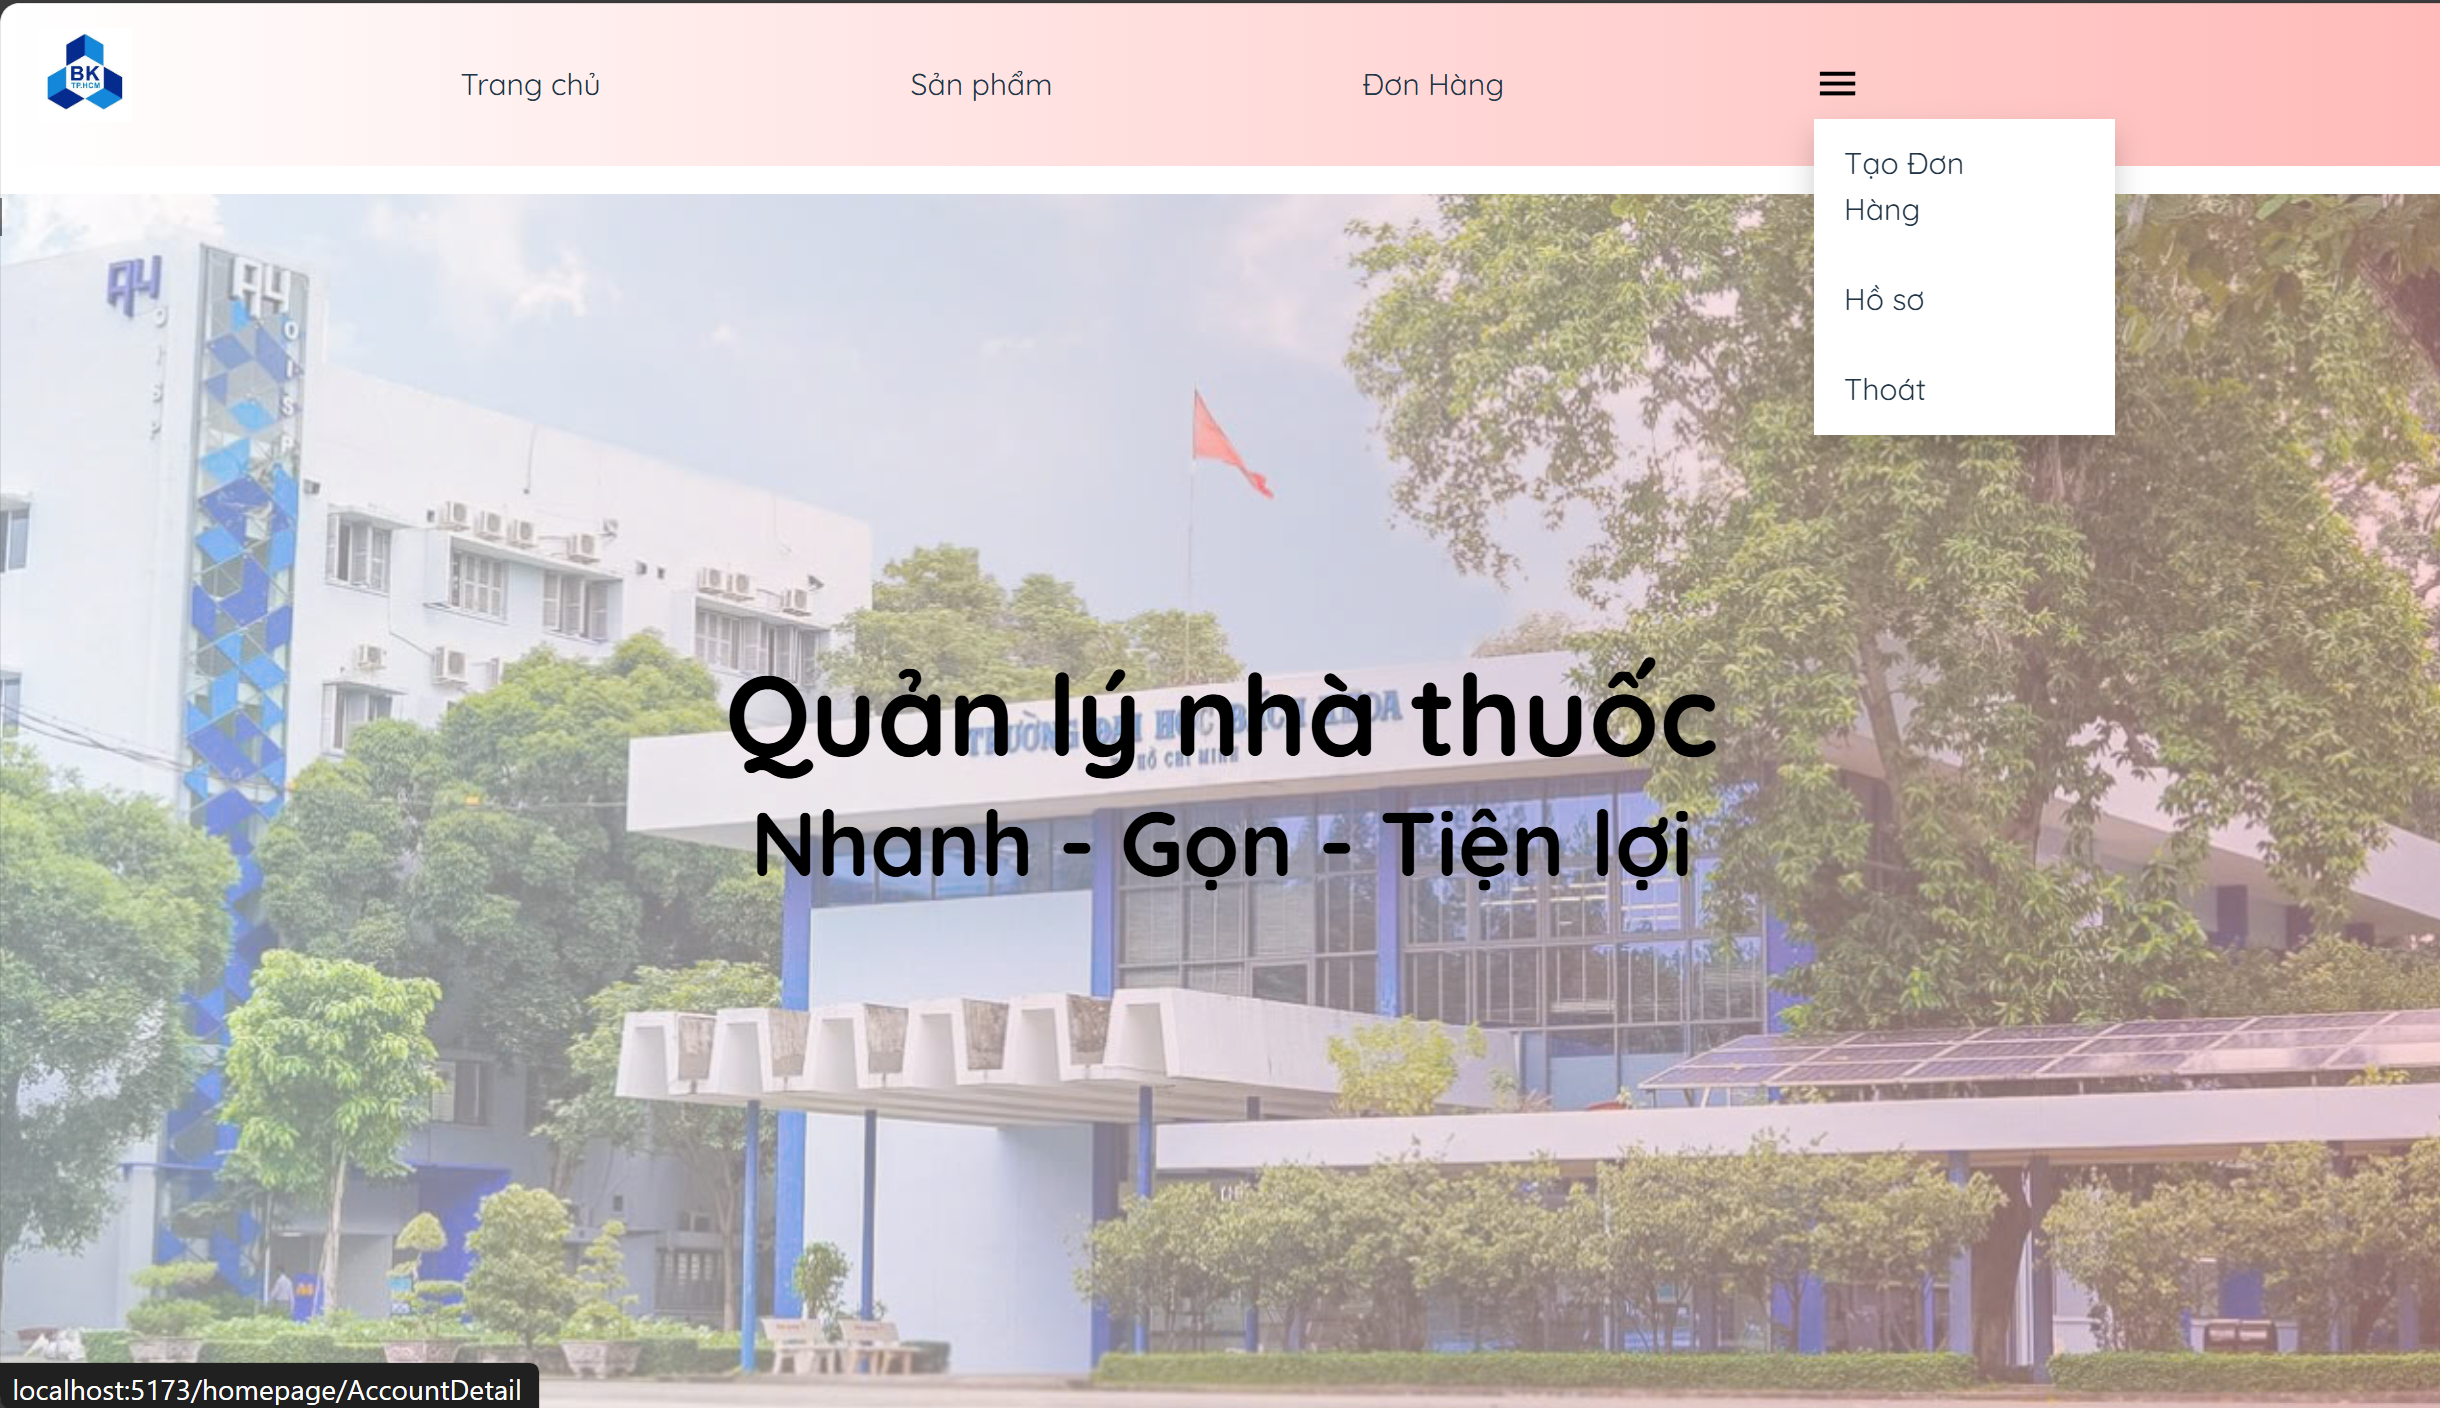
\includegraphics[scale=0.3]{Images/hp_pharmacist.png}
        \end{figure}
\end{itemize}
\subsection{Nhân viên}
Tại trang nhân viên sẽ hiển thị các tài khoản của nhân viên trong hệ thống kèm các chức năng:
\begin{itemize}
    \item Tìm kiếm nhân viên:
     \begin{figure}[H]
        \hspace*{1cm}     
            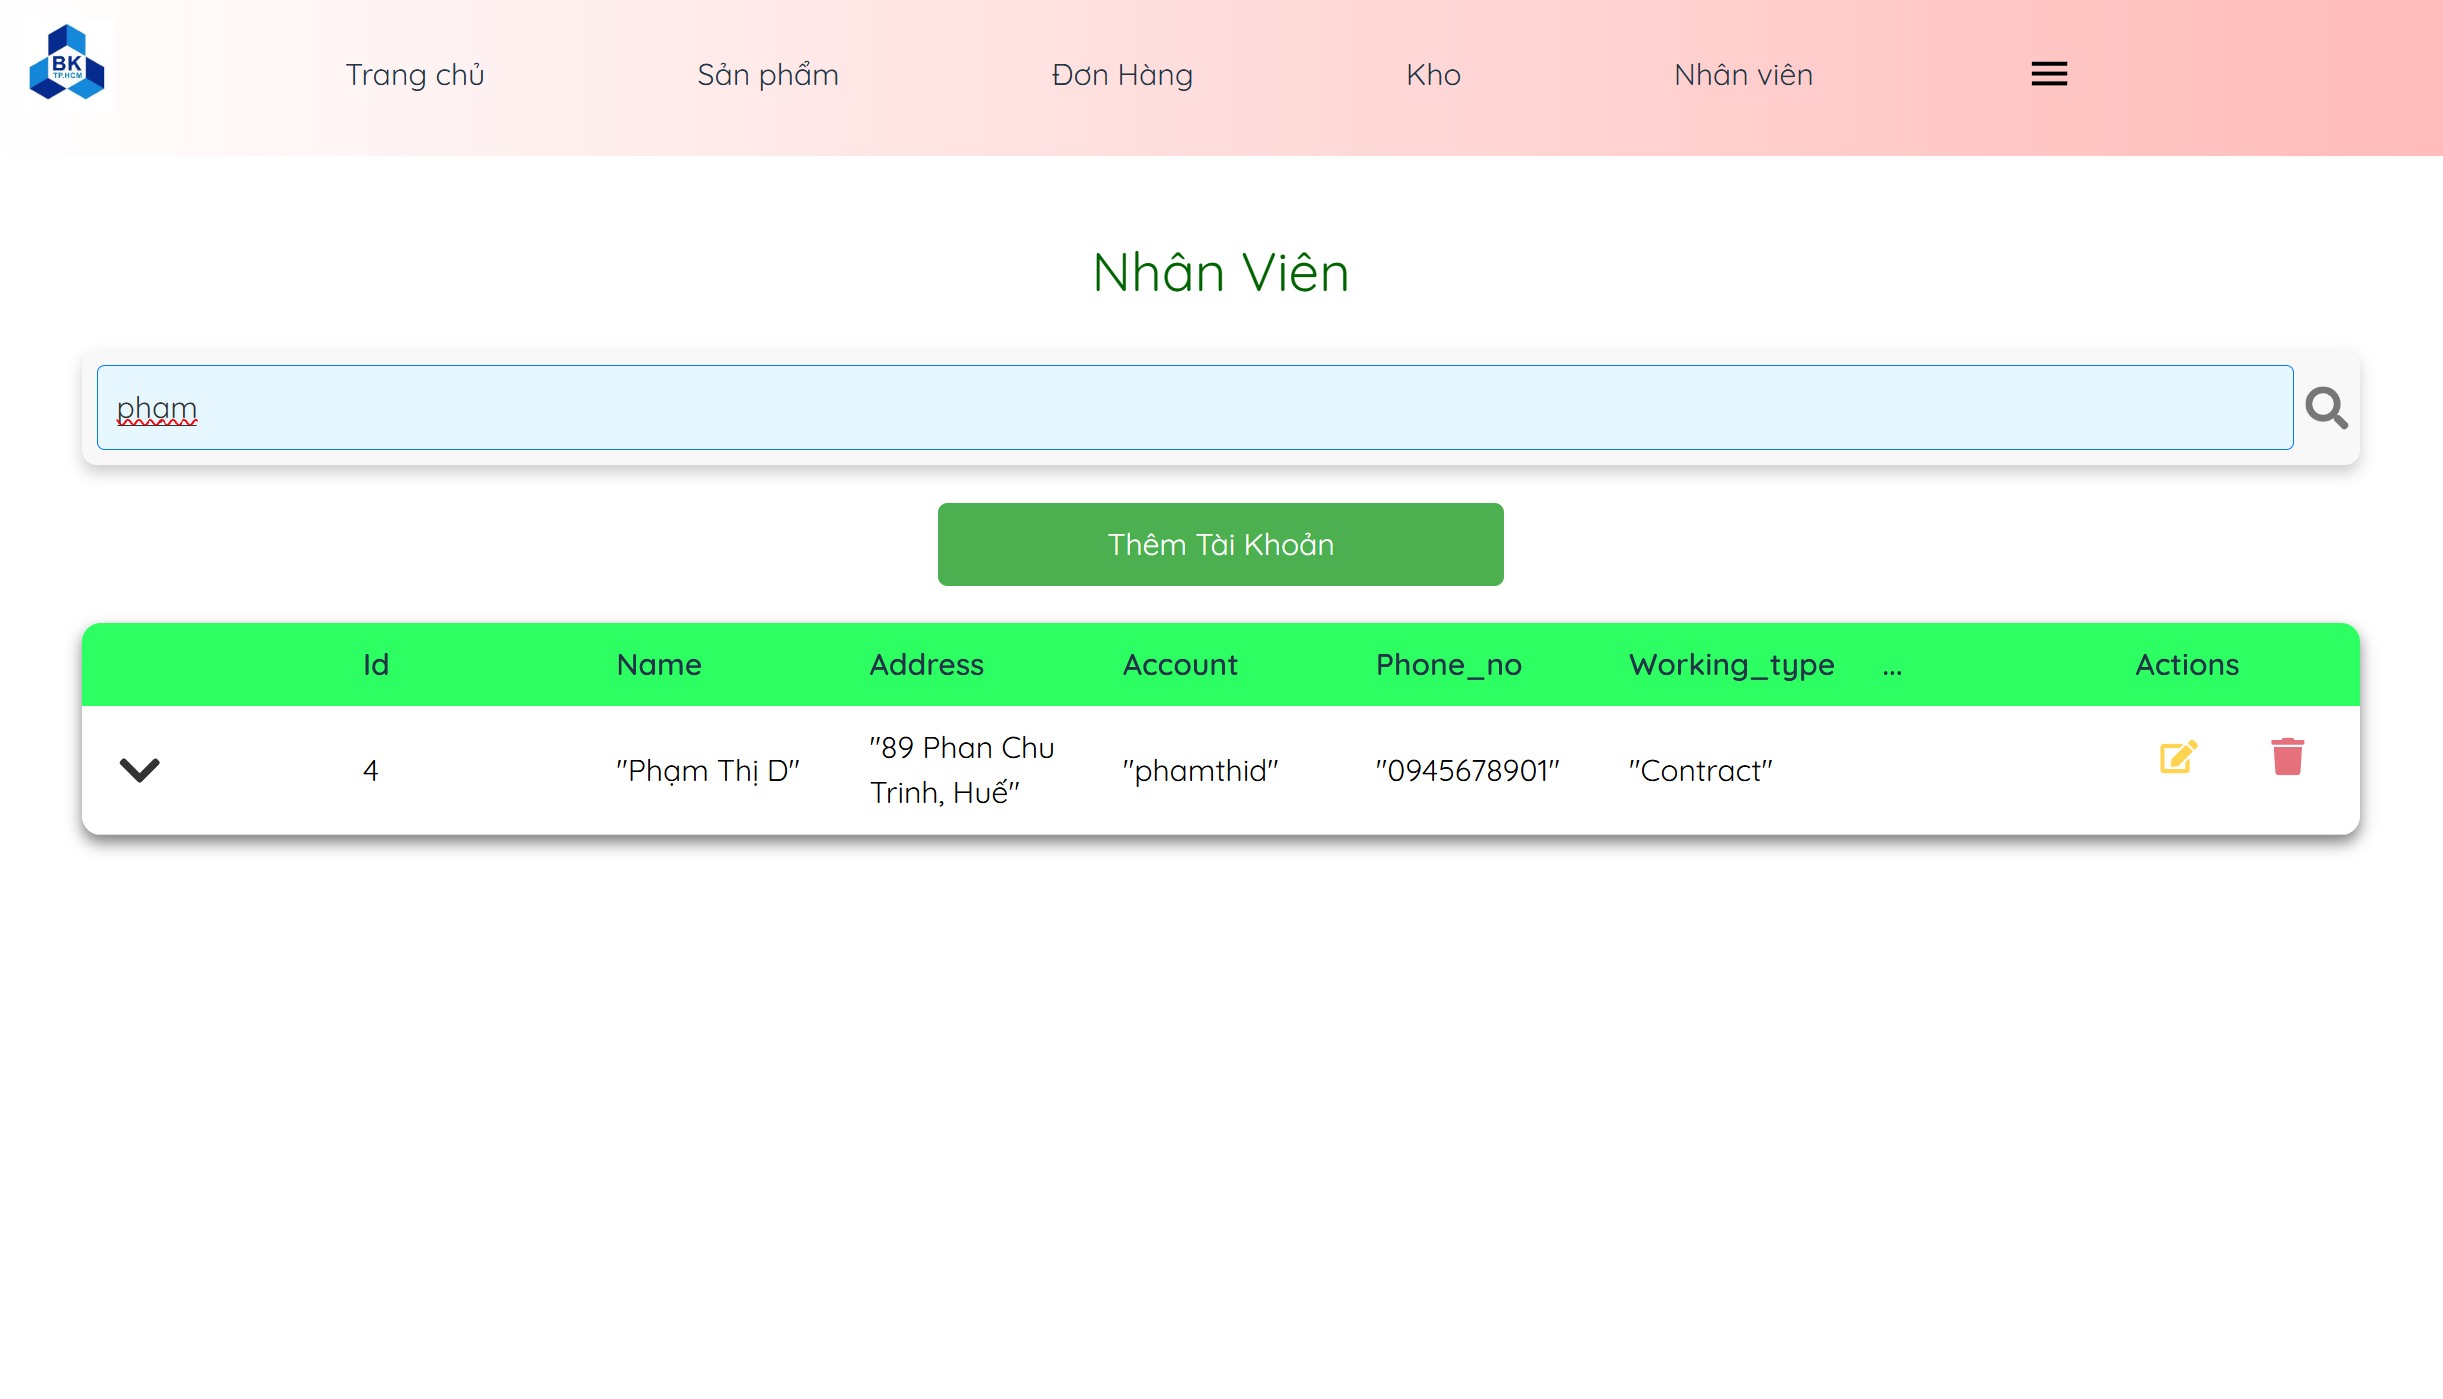
\includegraphics[scale=0.3]{Images/search_nv.png}
        \end{figure}
    \item Xóa nhân viên:
     \begin{figure}[H]
        \hspace*{1cm}     
            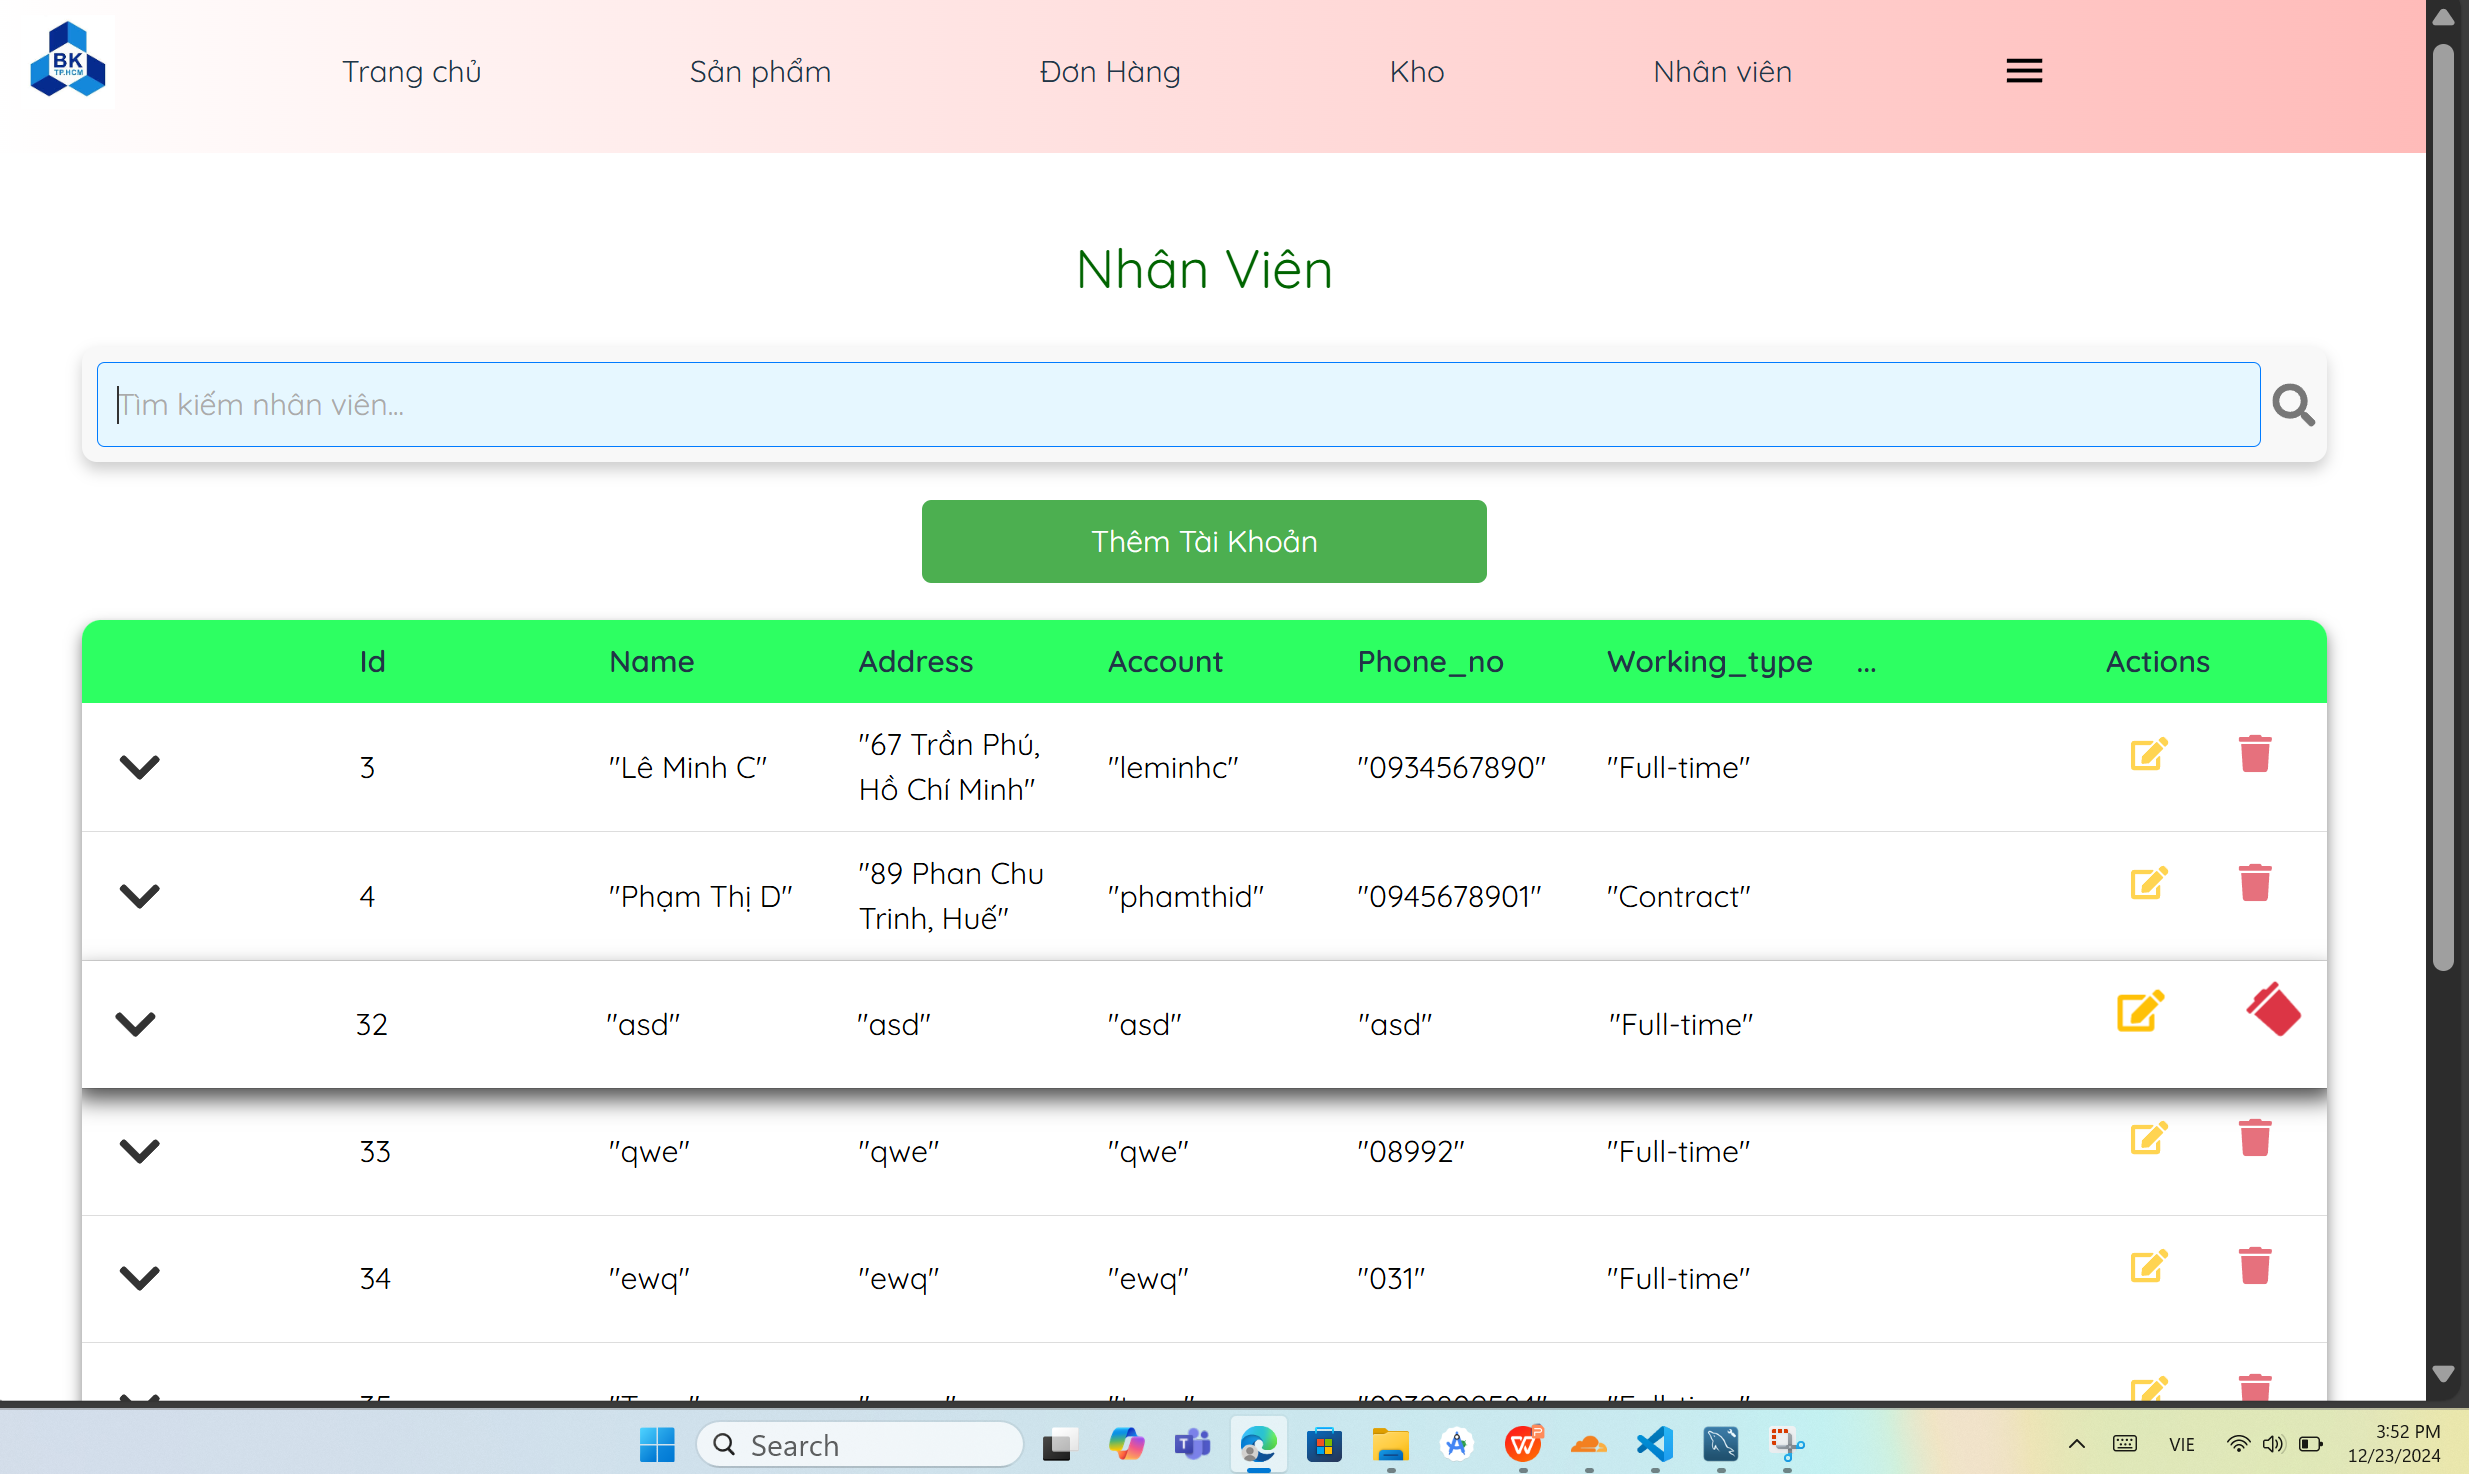
\includegraphics[scale=0.3]{Images/xoanv.png}
        \end{figure}
        Nhân viên đã được xóa thành công:
        \begin{figure}[H]
        \hspace*{1cm}     
            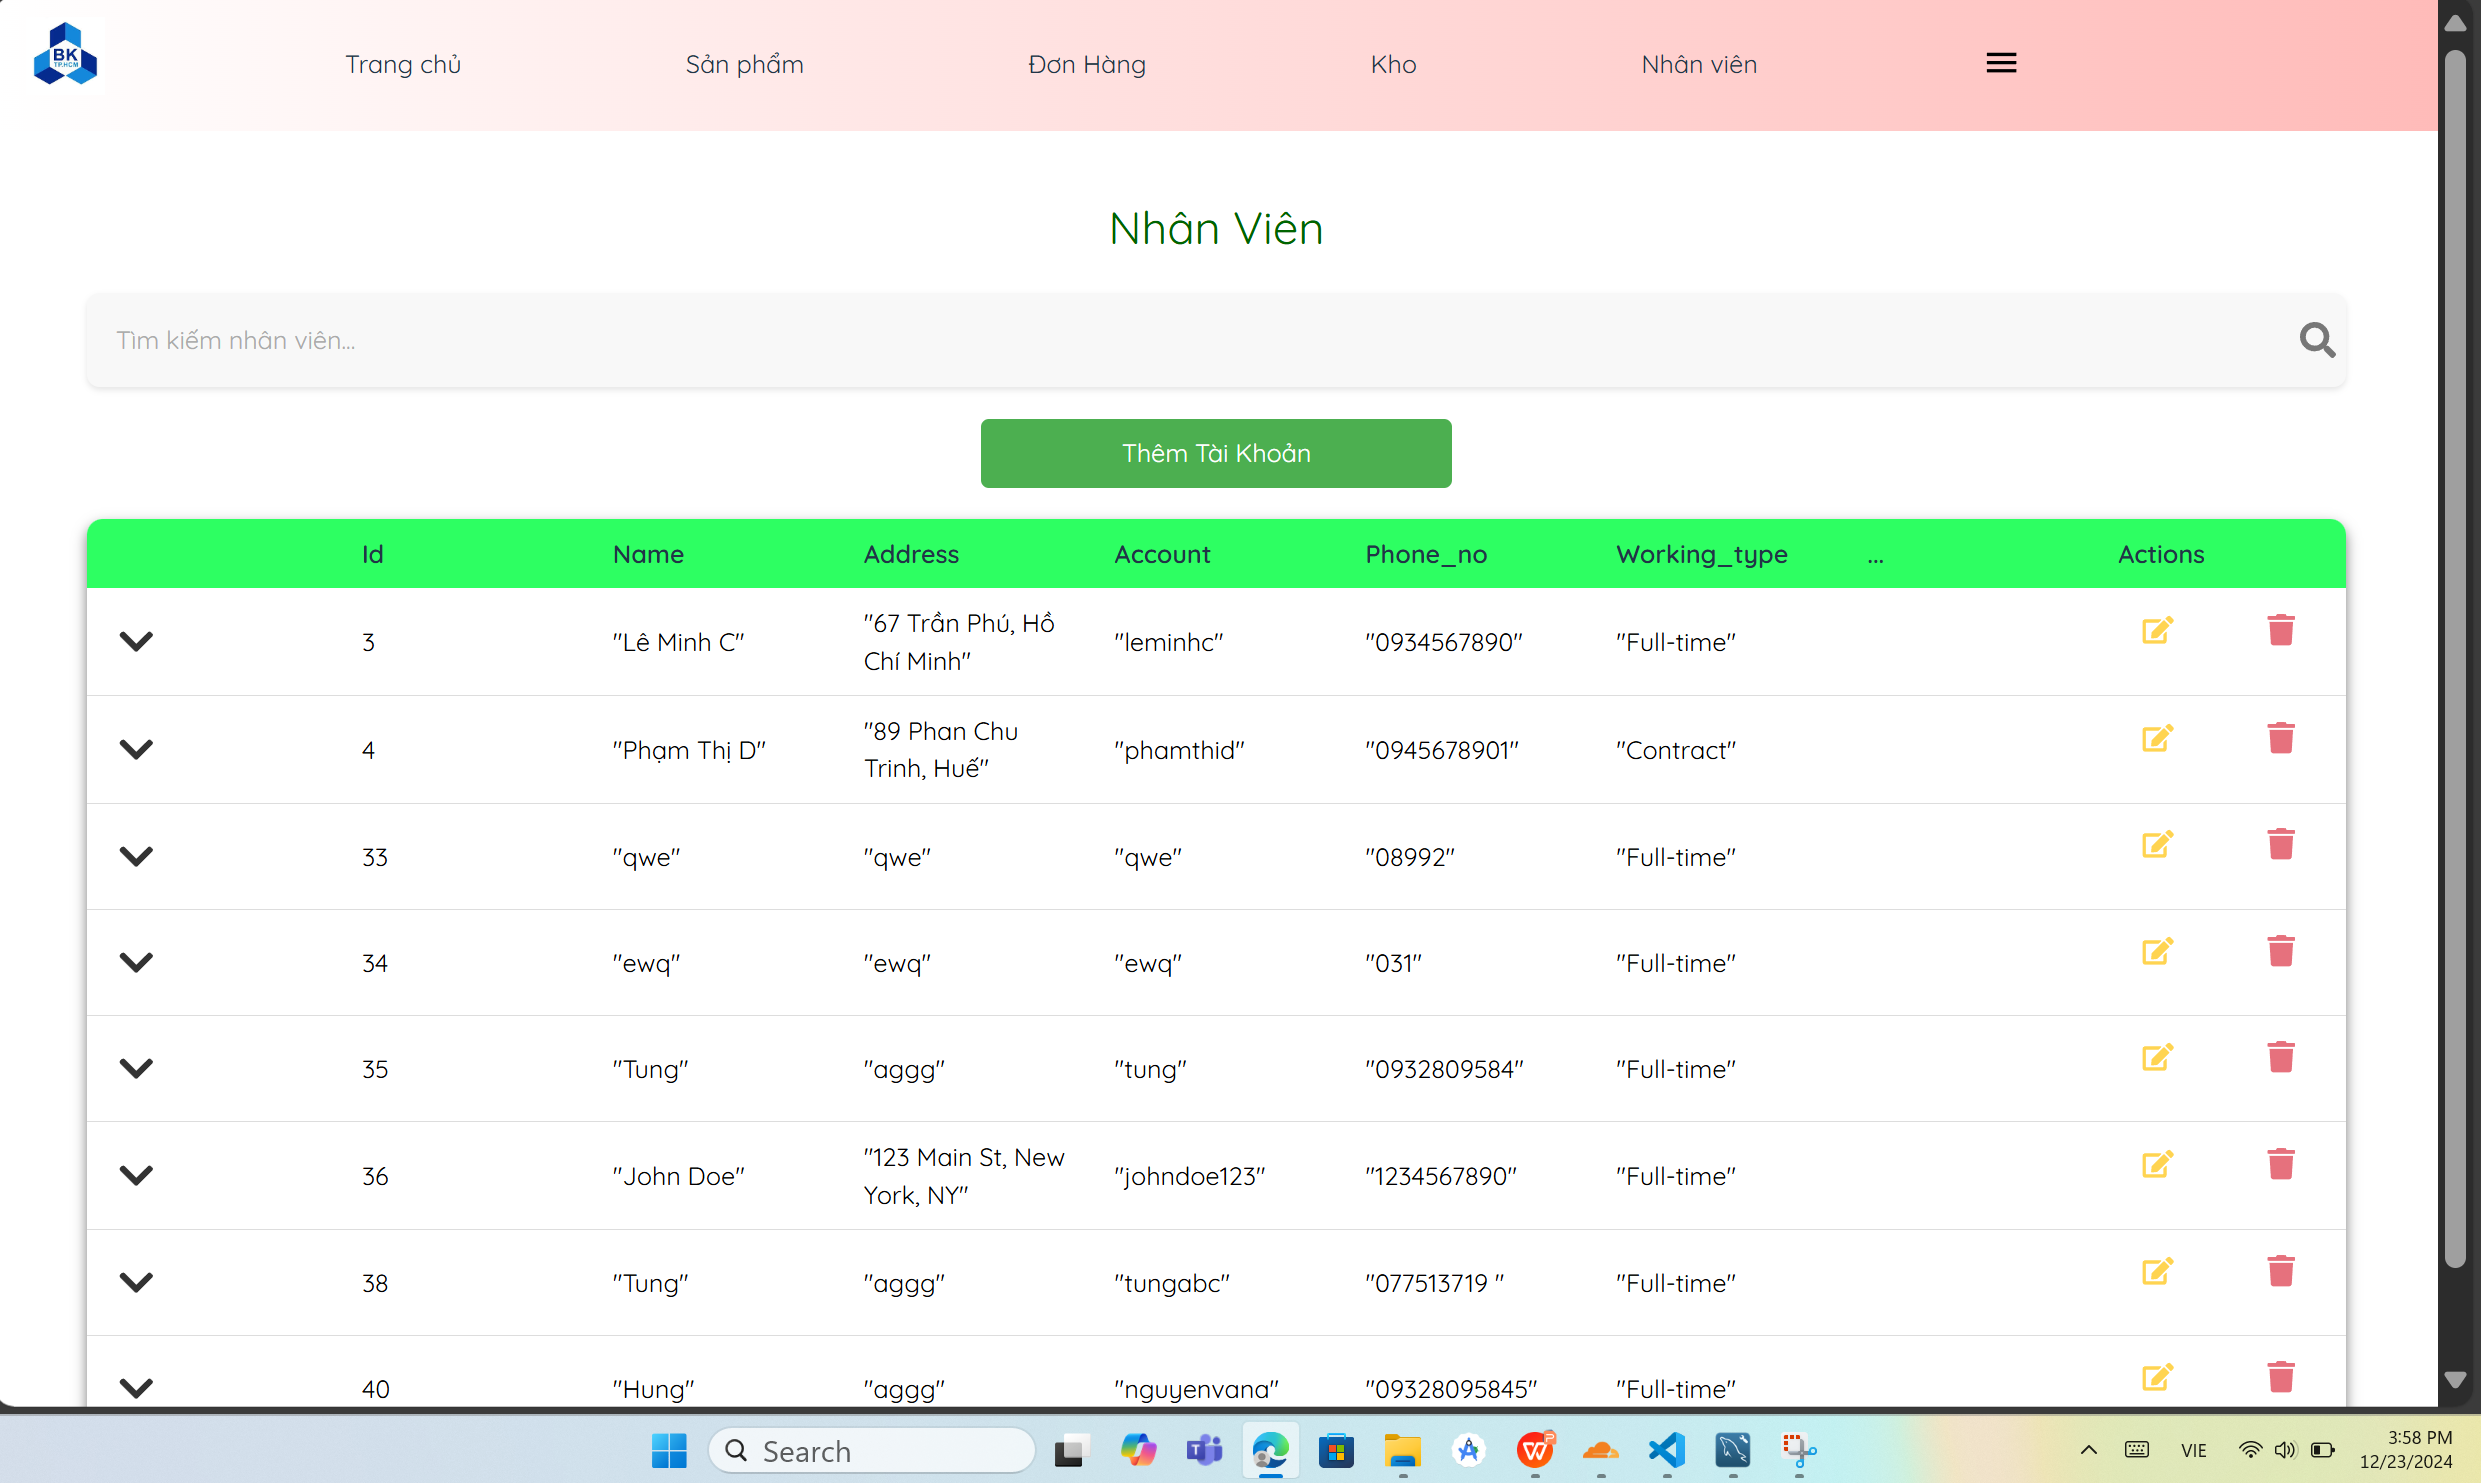
\includegraphics[scale=0.3]{Images/nvbay.png}
        \end{figure}
    \item Sửa thông tin nhân viên:
    \begin{figure}[H]
        \hspace*{-1cm}     
            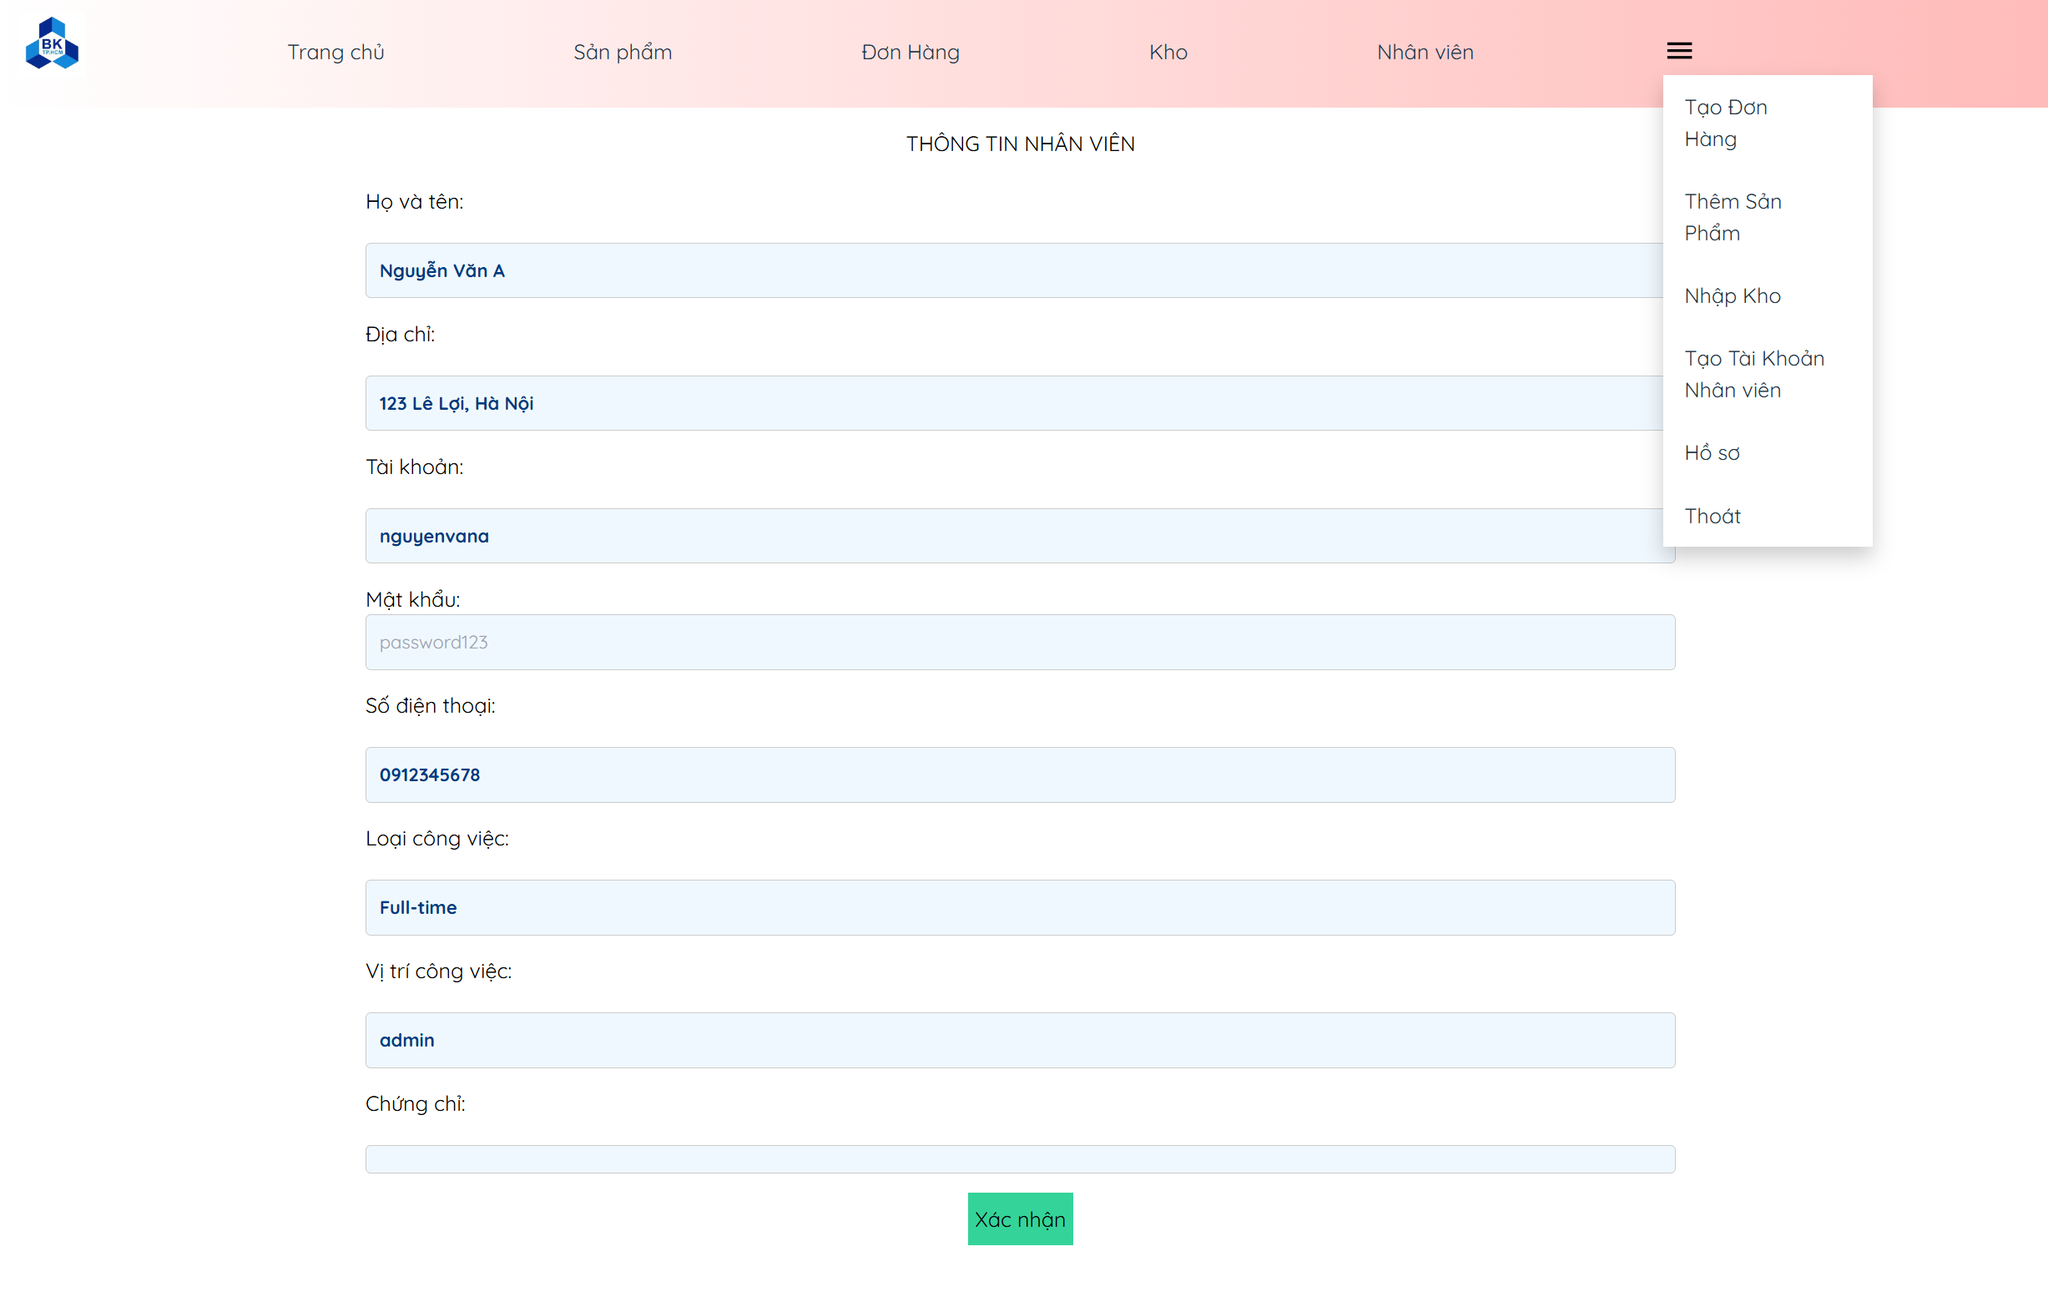
\includegraphics[scale=0.2]{Images/pas_hoso.png}
        \end{figure}
    \item Thêm nhân viên: 

         \begin{figure}[H]
        \hspace*{1cm}     
            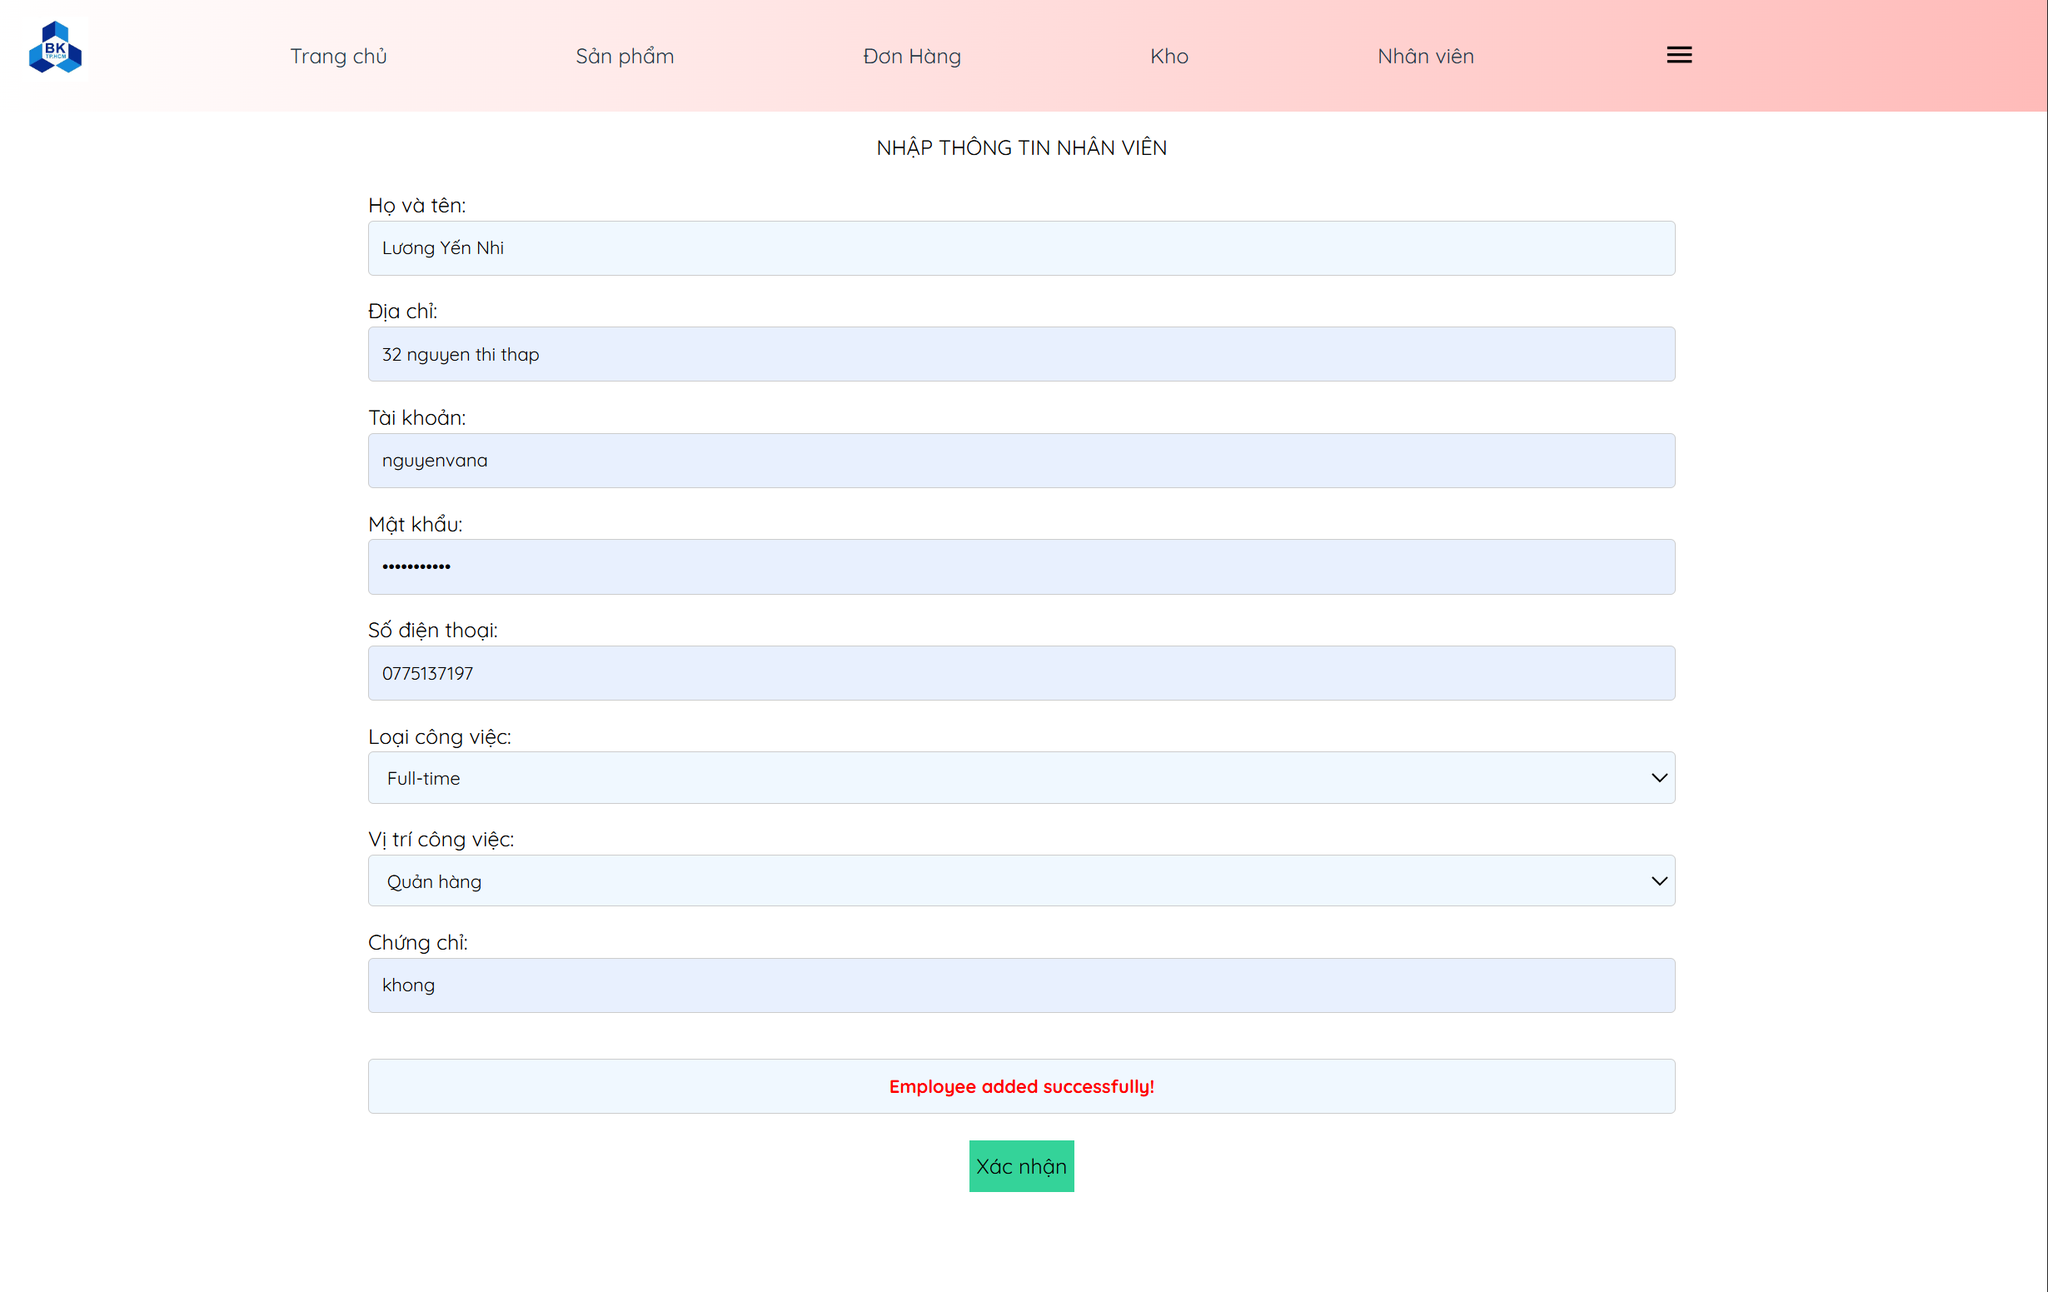
\includegraphics[scale=0.2]{Images/insert_nv_2.png}
        \end{figure}

          \begin{figure}[H]
        \hspace*{1.9cm}     
            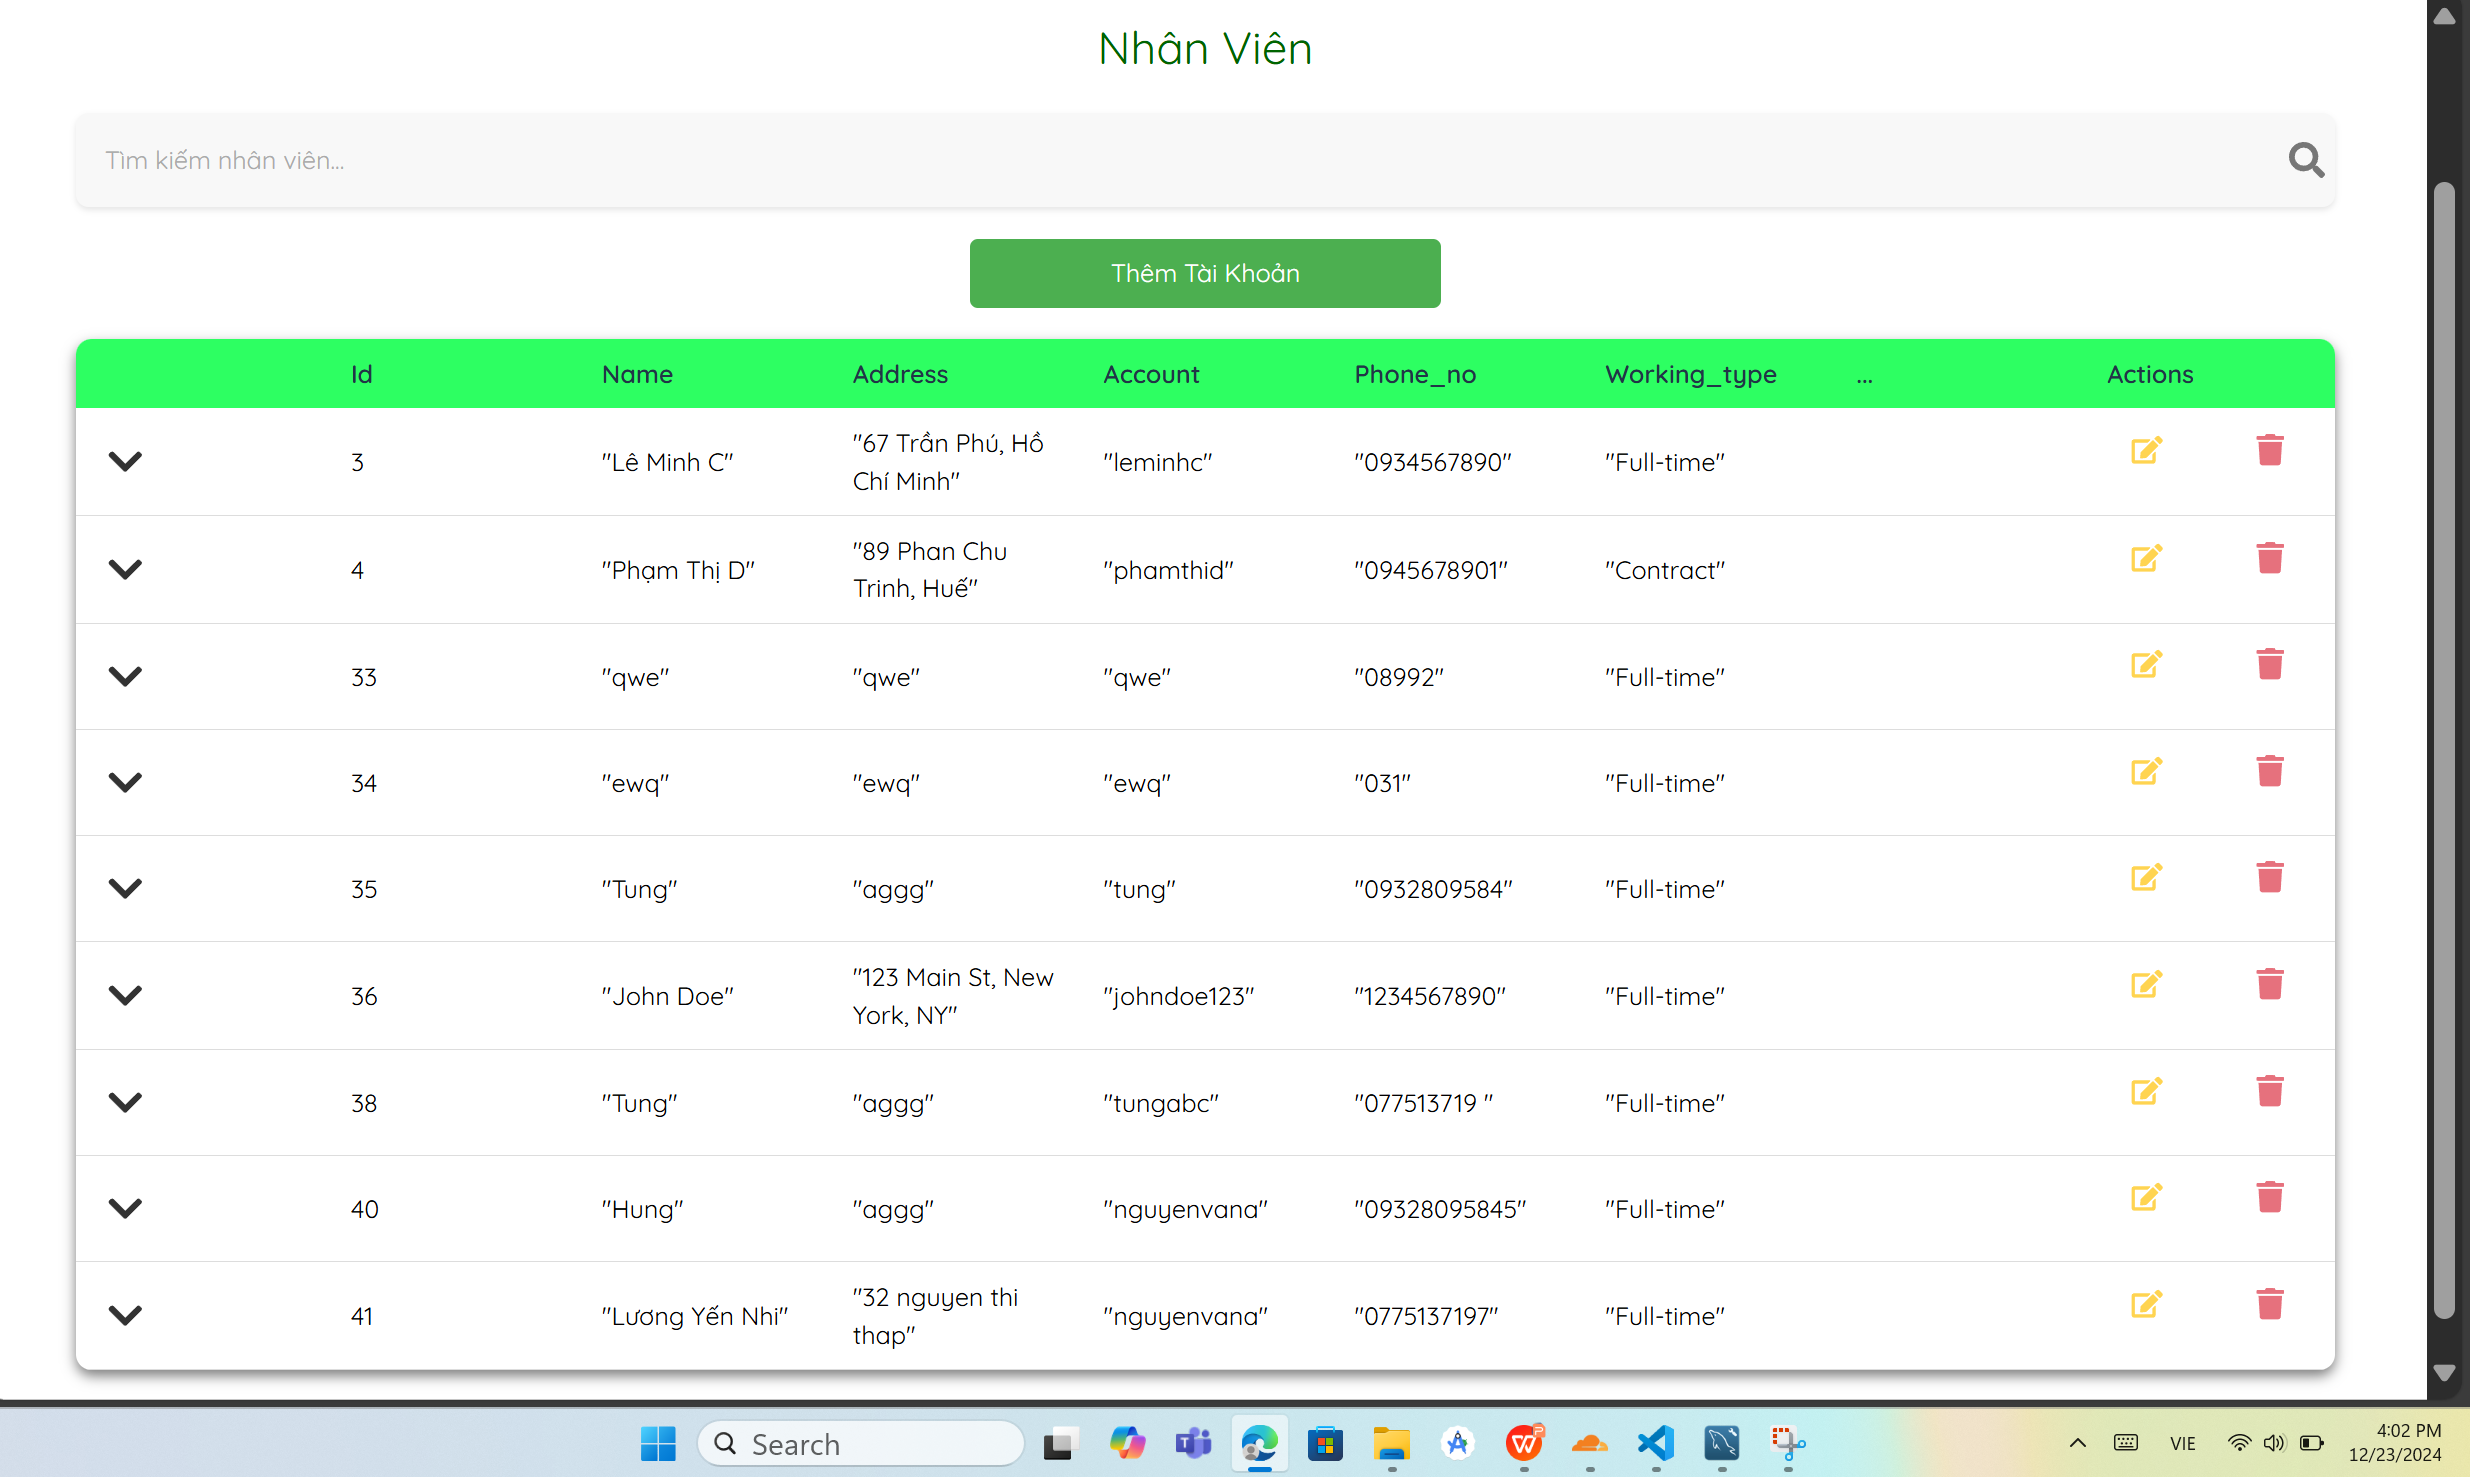
\includegraphics[scale=0.3]{Images/insert_r.png}
        \end{figure}
\end{itemize}
\subsection{Tạo đơn hàng (Nhân viên bán thuốc)}
\textbf{Các đơn hàng đã được tạo trong hệ thống:}
  \begin{figure}[H]  
          \hspace*{1cm}     
            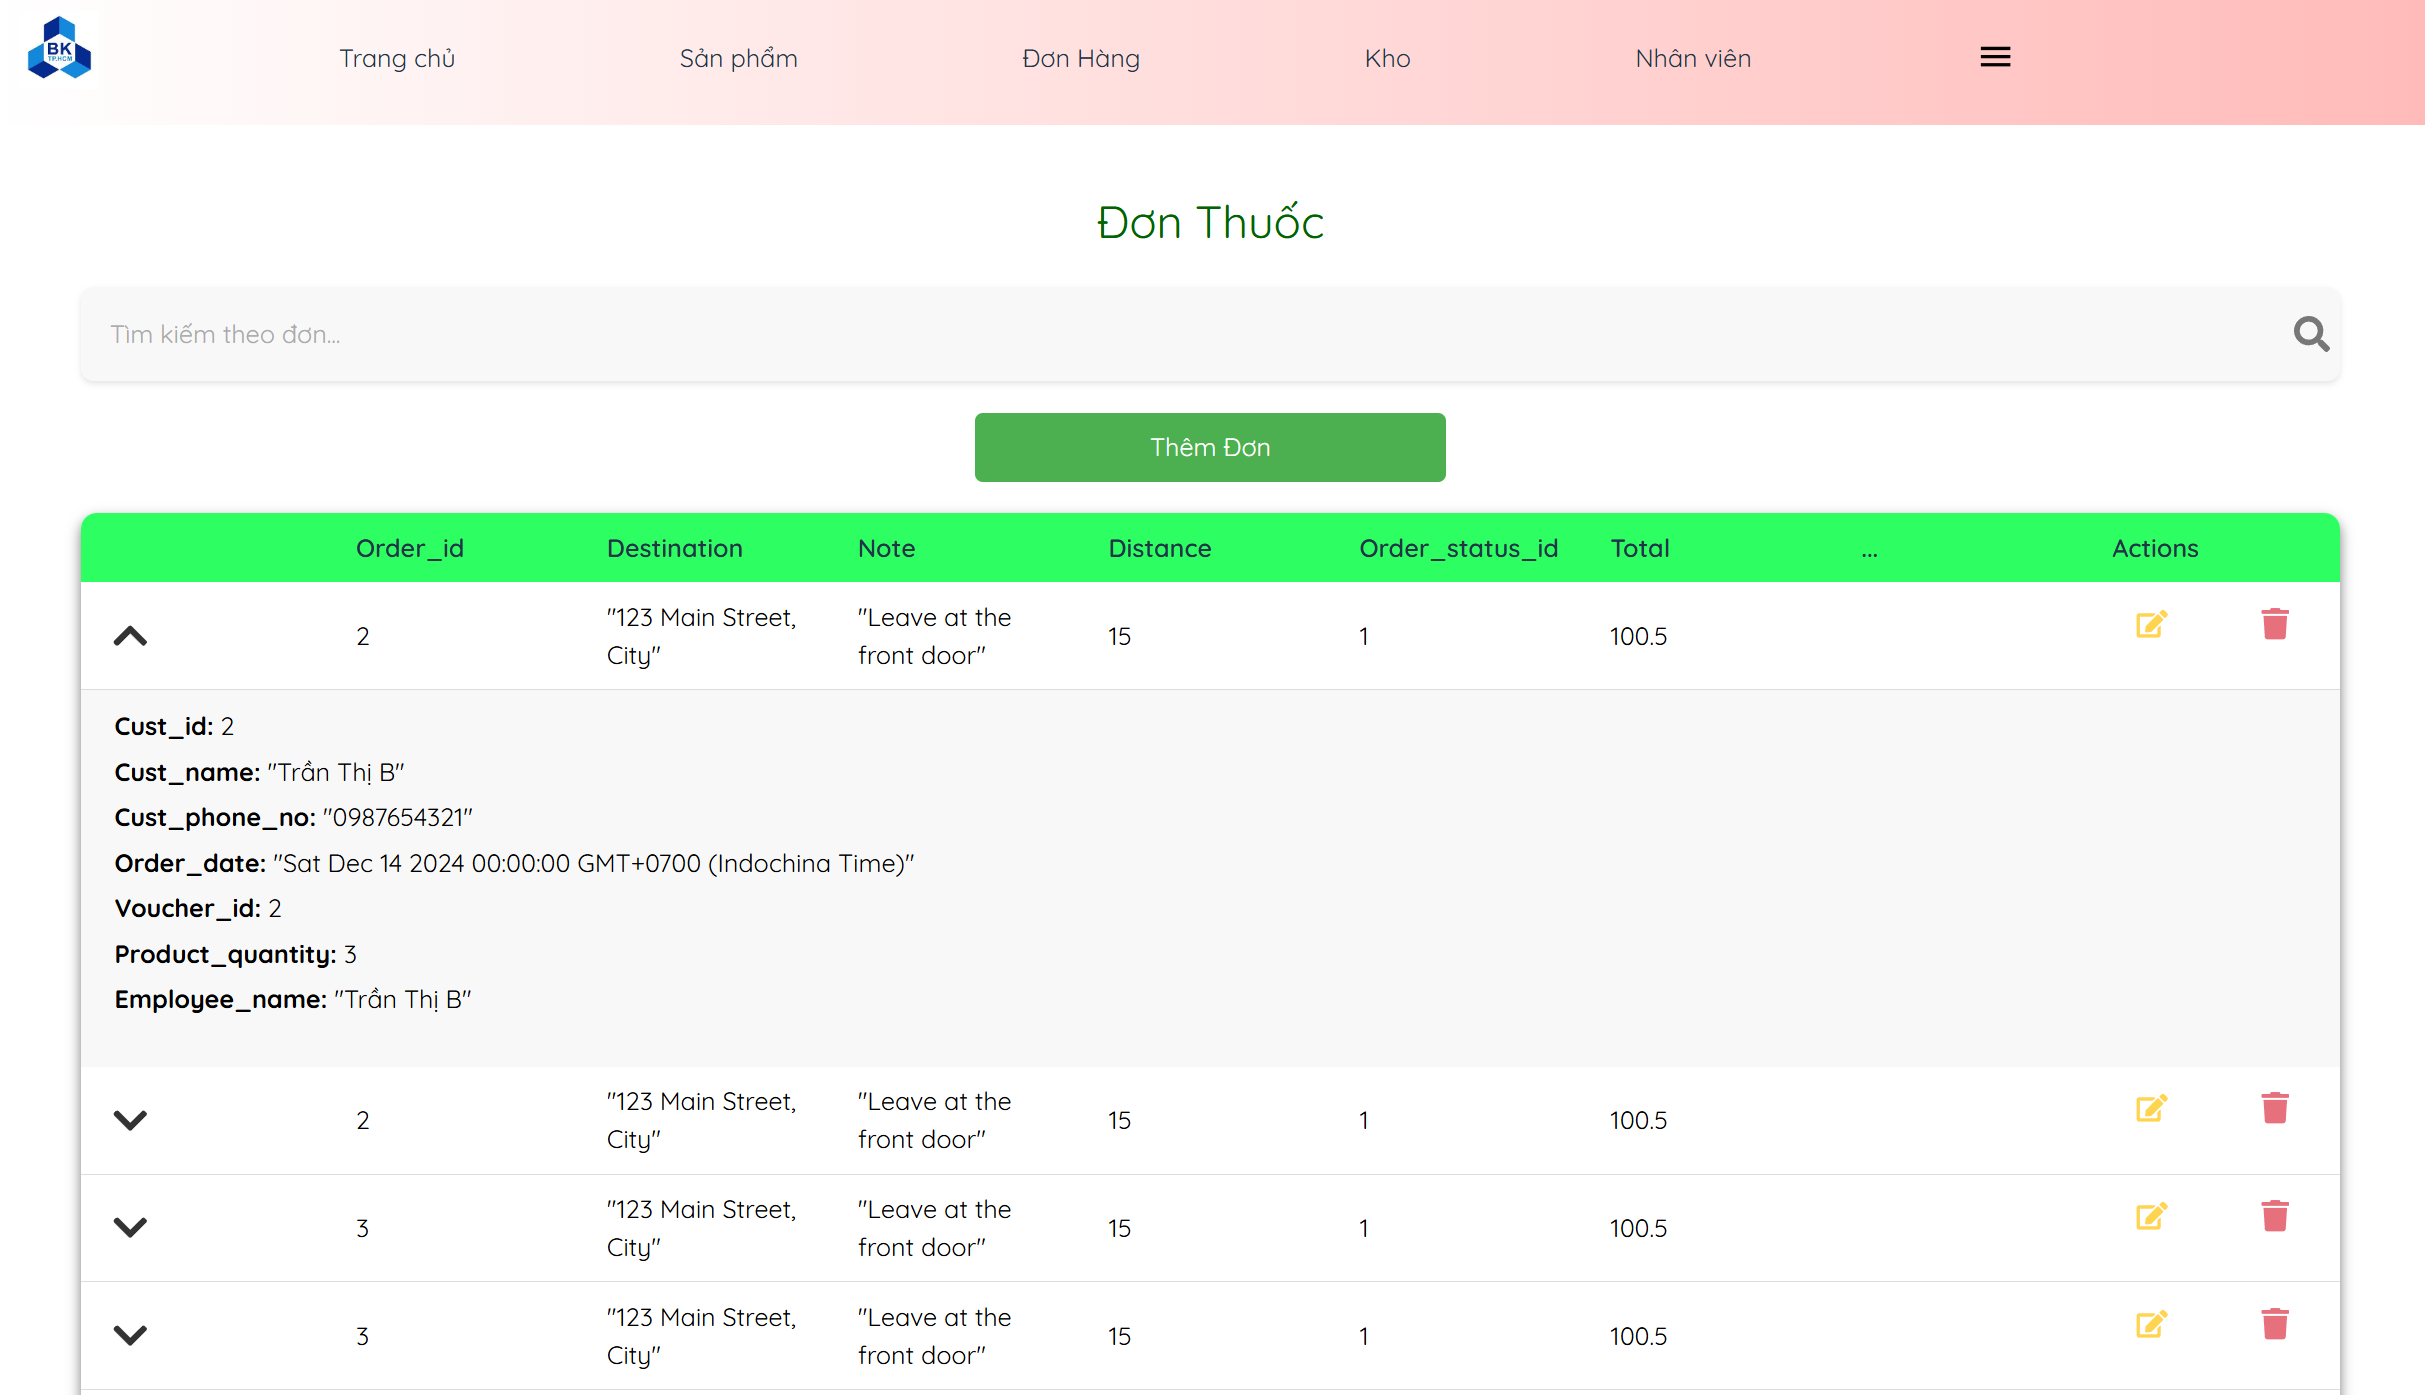
\includegraphics[scale=0.3]{Images/showdon.png}
        \end{figure}
Để thuận tiện, hệ thống sẽ cho người dùng chọn trước các sản phẩm mình muốn chọn:
  \begin{figure}[H]
        \hspace*{-1cm}     
            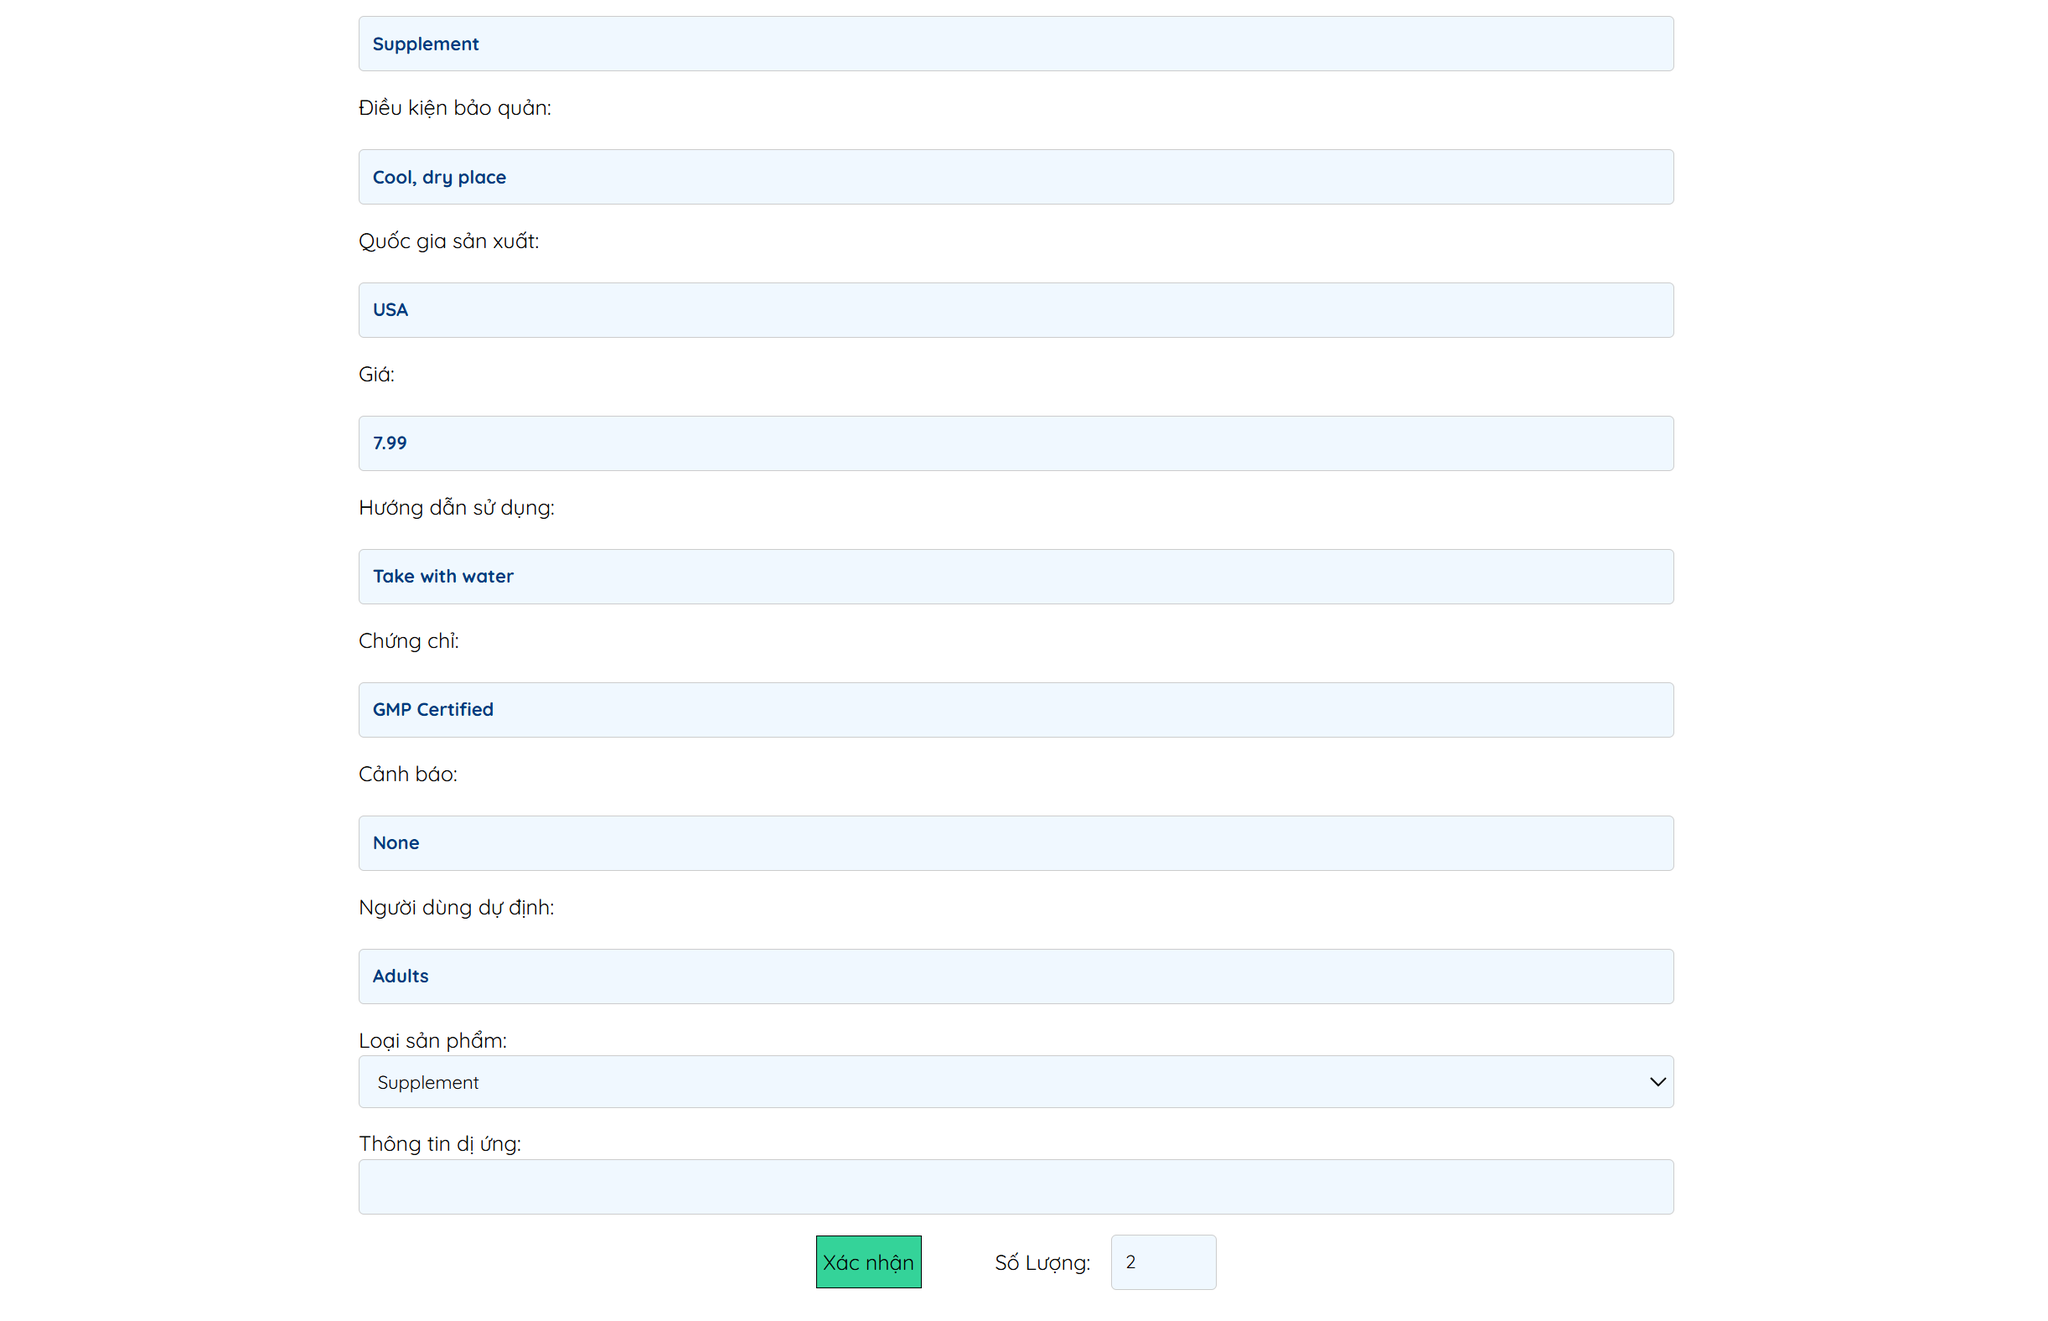
\includegraphics[scale=0.2]{Images/add_sp.png}
        \end{figure}
        
          \begin{figure}[H]  
        \hspace*{-3cm}     
            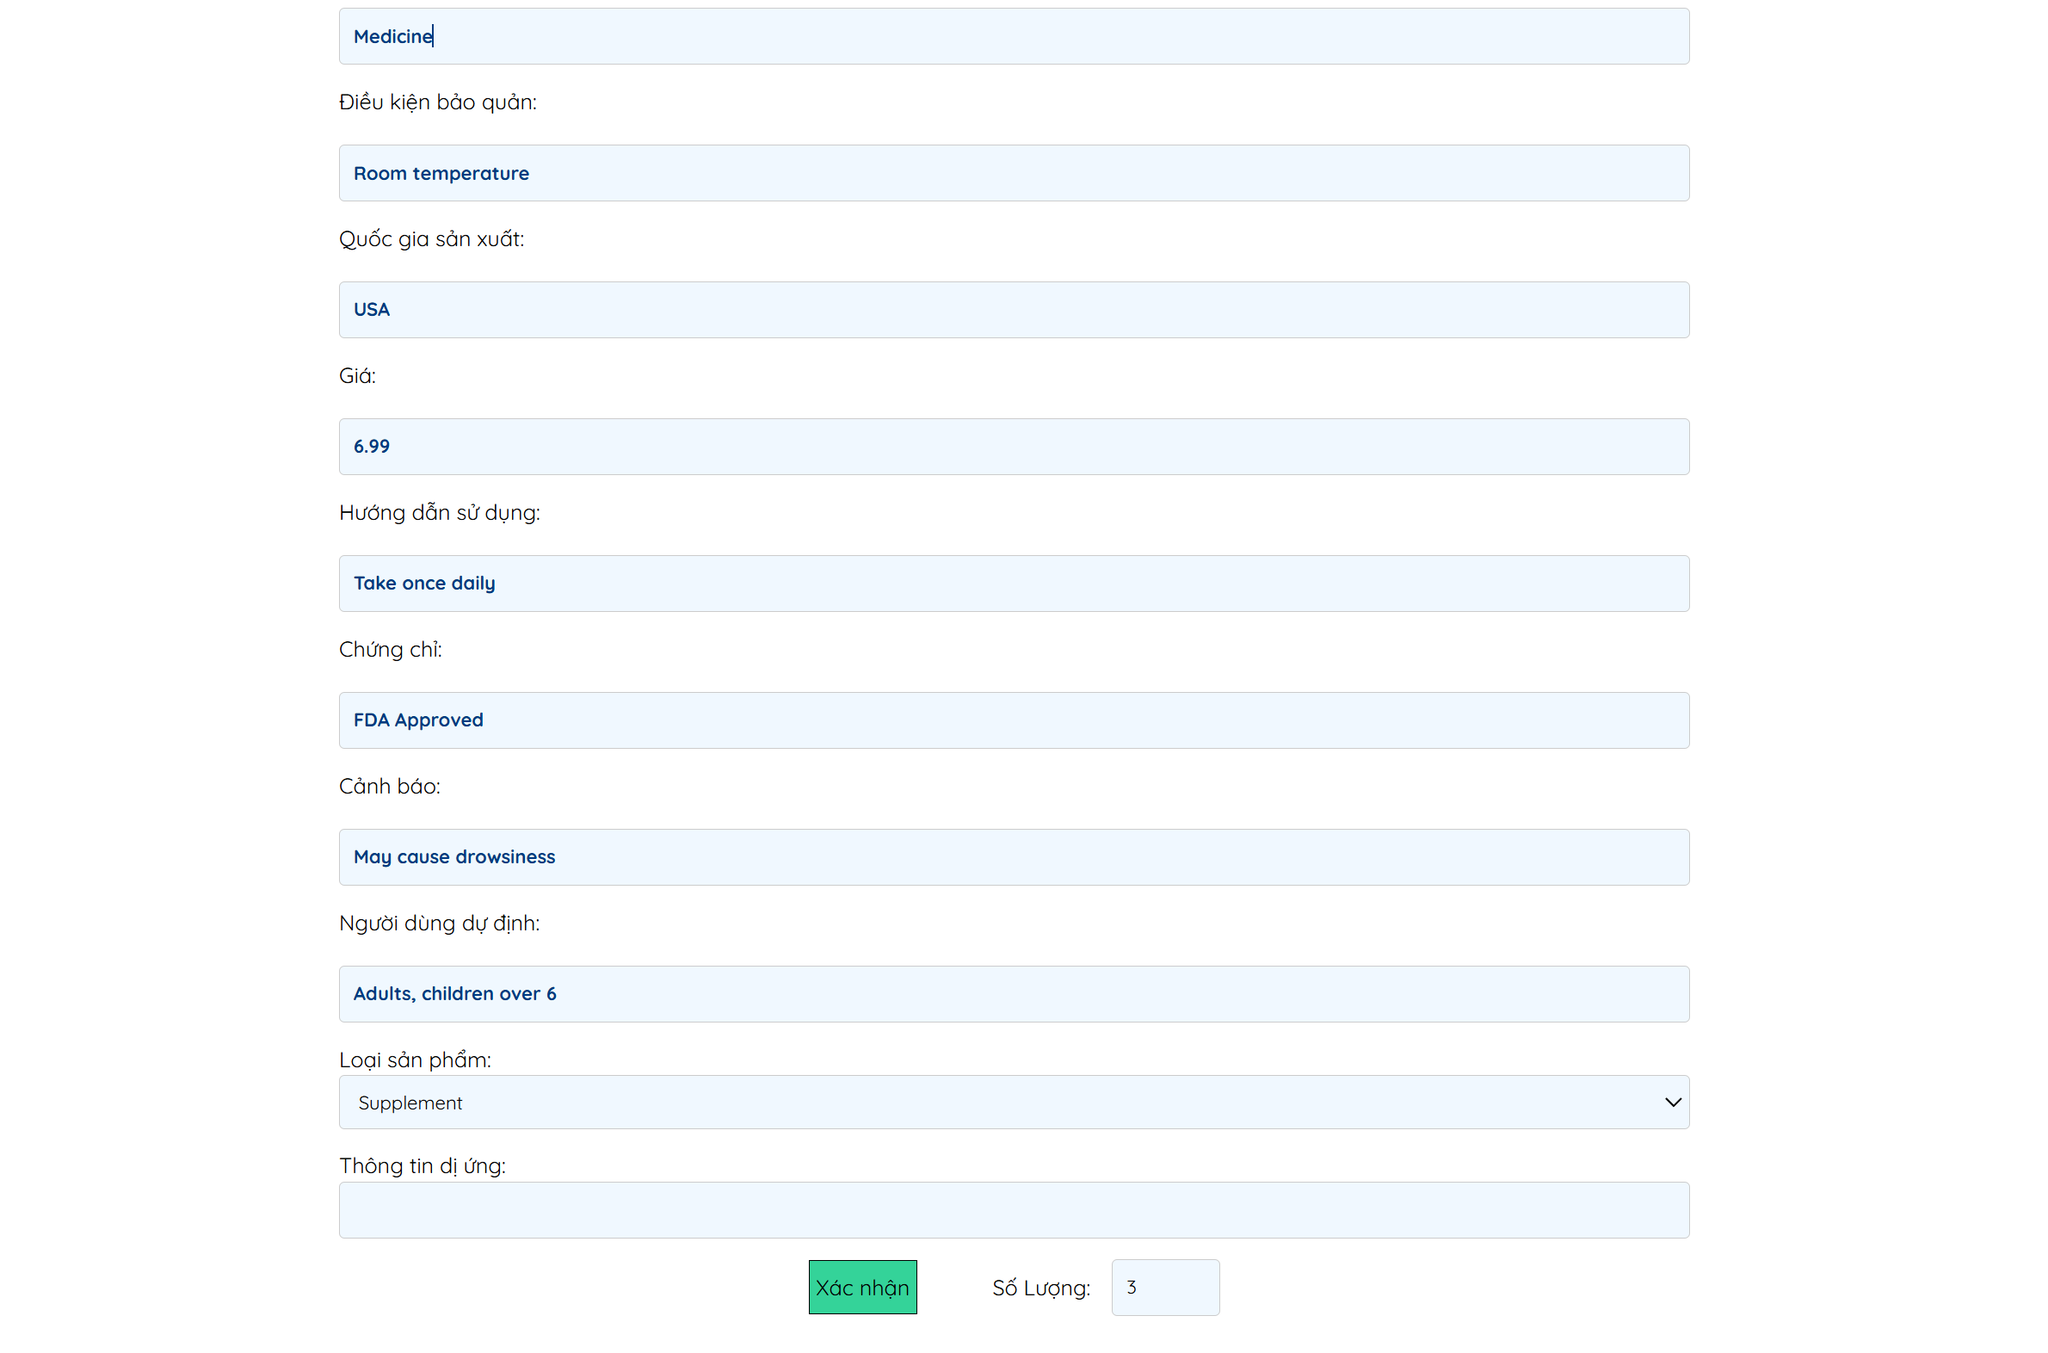
\includegraphics[scale=0.3]{Images/add_pro2.png}
        \end{figure}

         \begin{figure}[H]  
        \hspace*{-3cm}     
            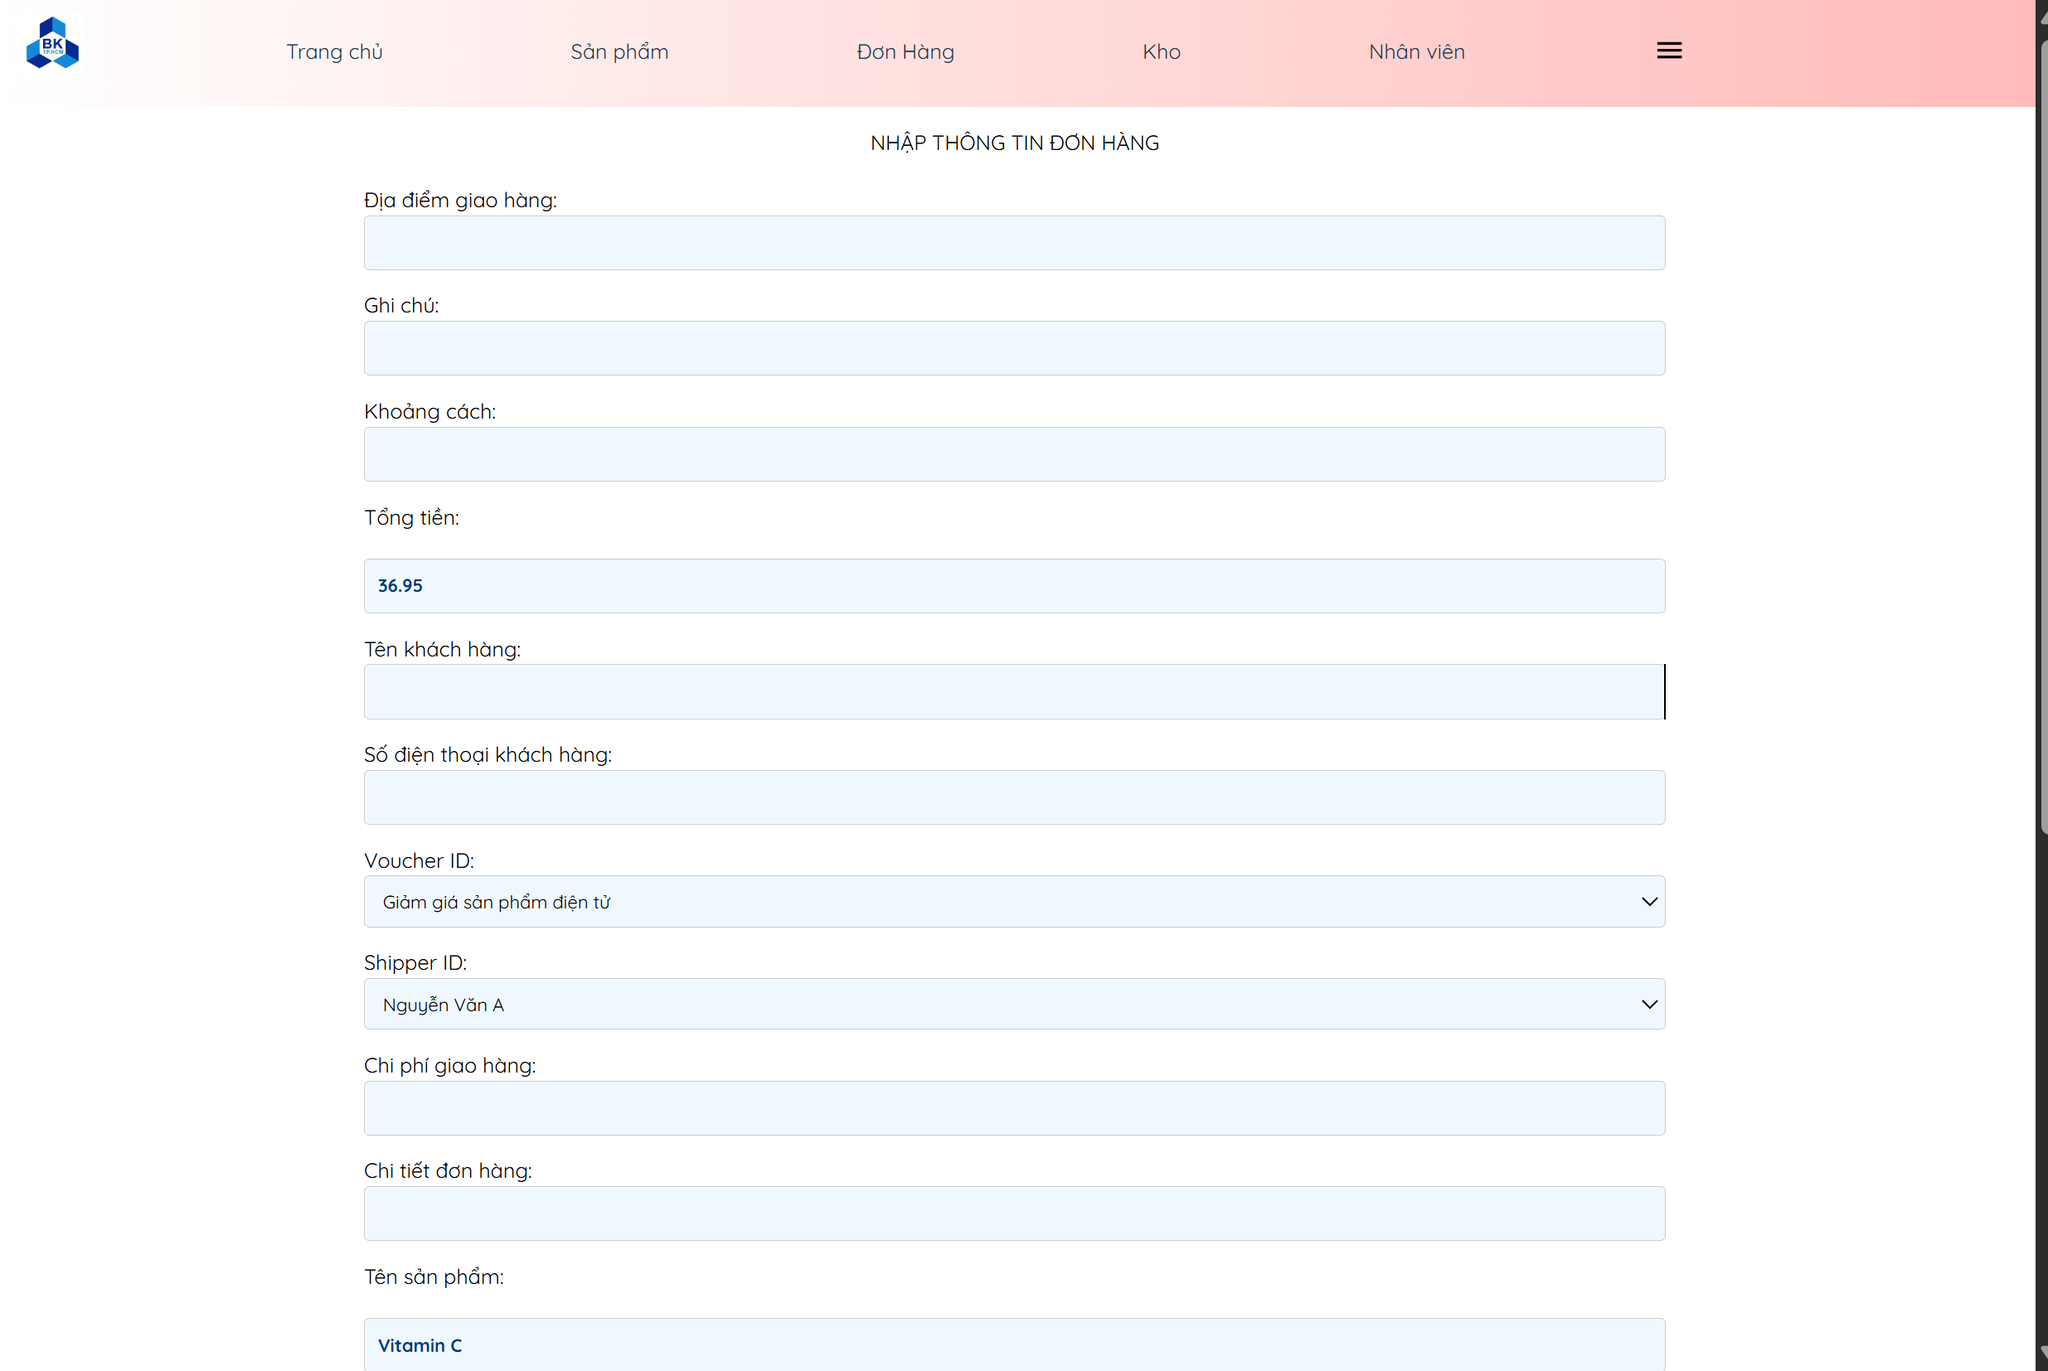
\includegraphics[scale=0.26]{Images/insertDon1.png}
        \end{figure}

         \begin{figure}[H]  
        \hspace*{-3cm}     
            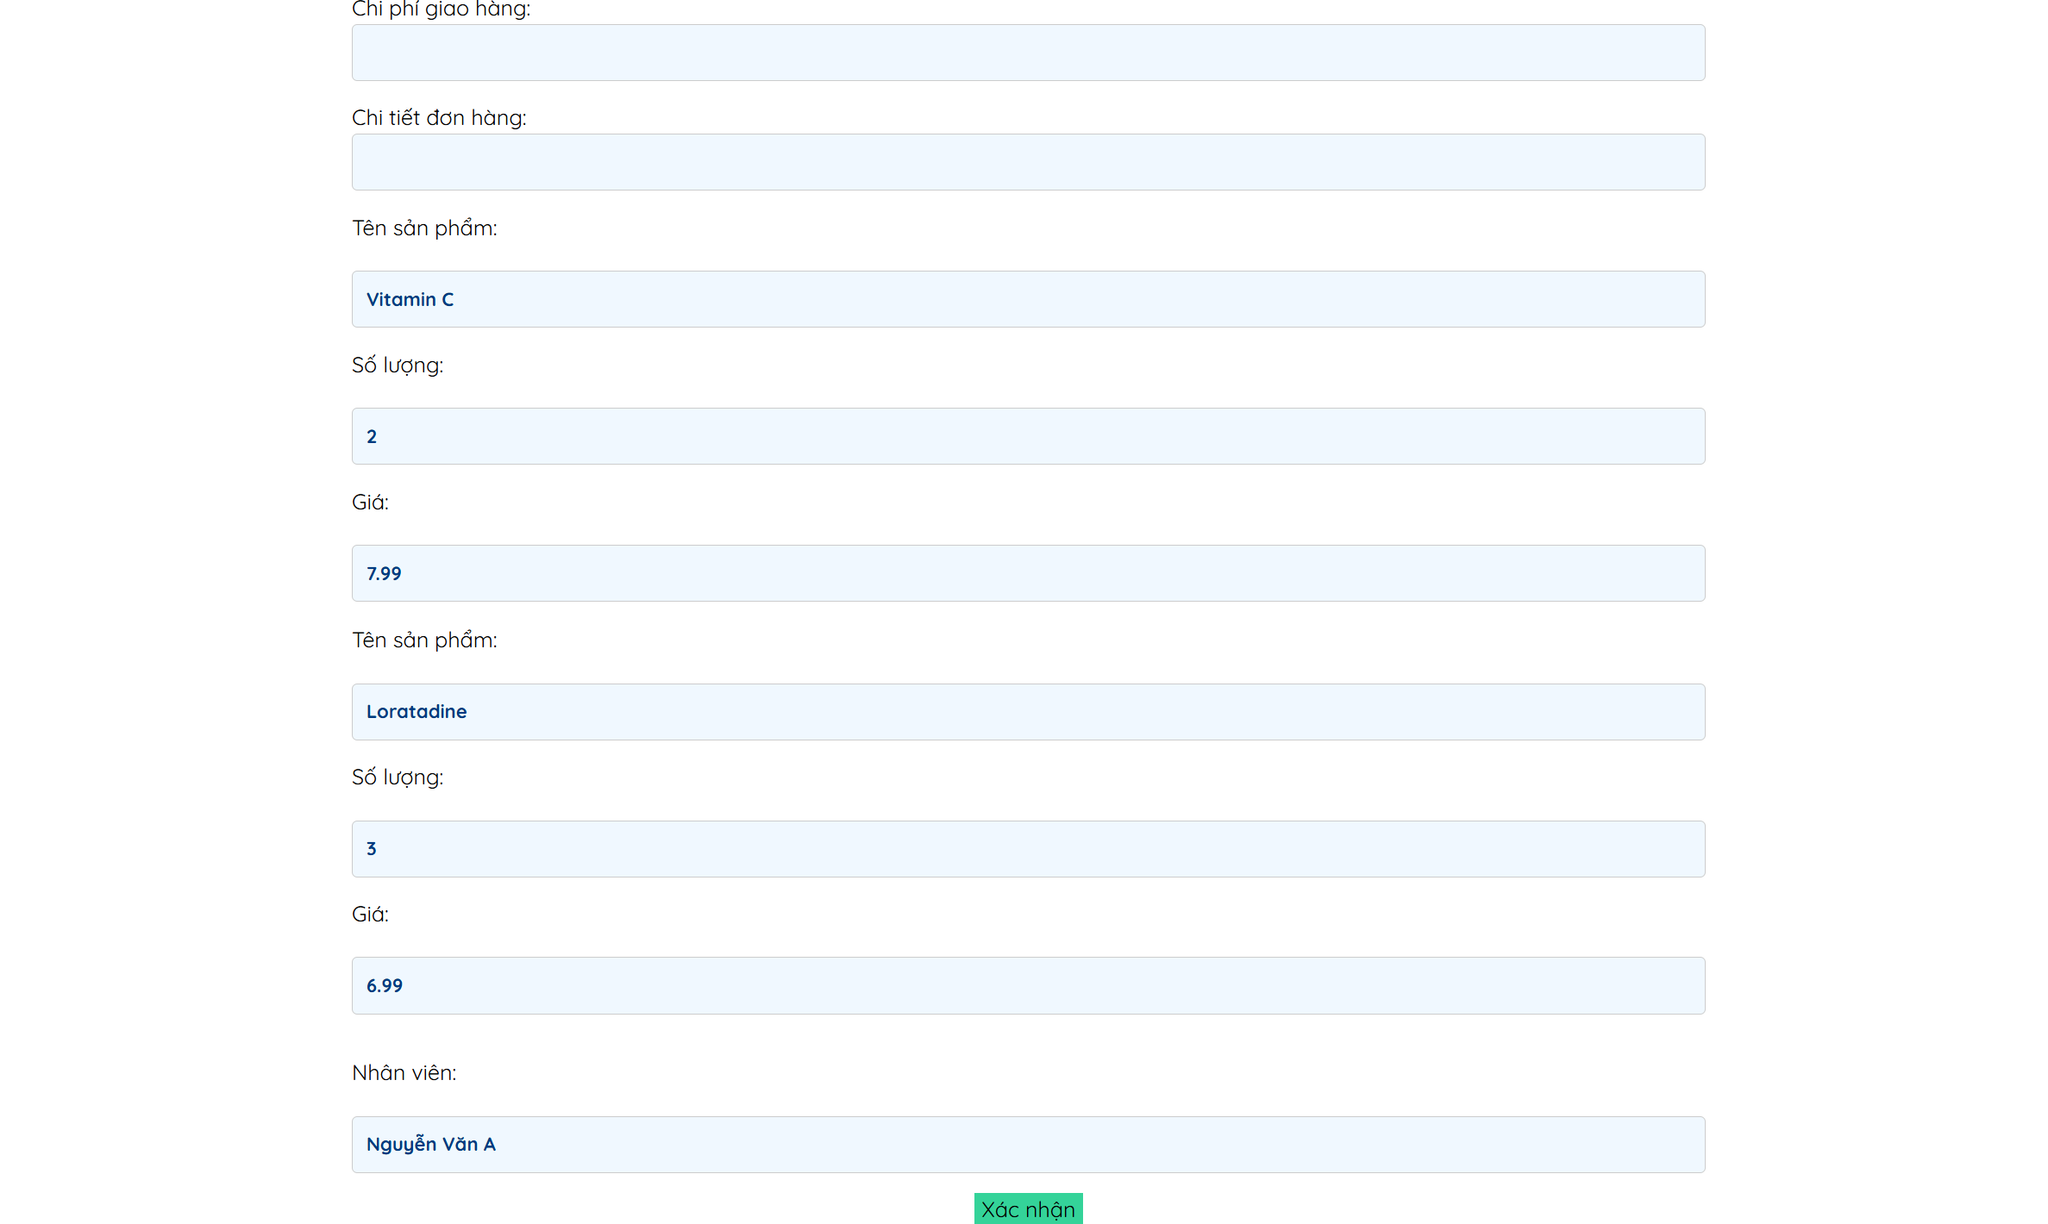
\includegraphics[scale=0.3]{Images/insertPhar2.png}
        \end{figure}

            \begin{figure}[H]  
        \hspace*{-3cm}     
            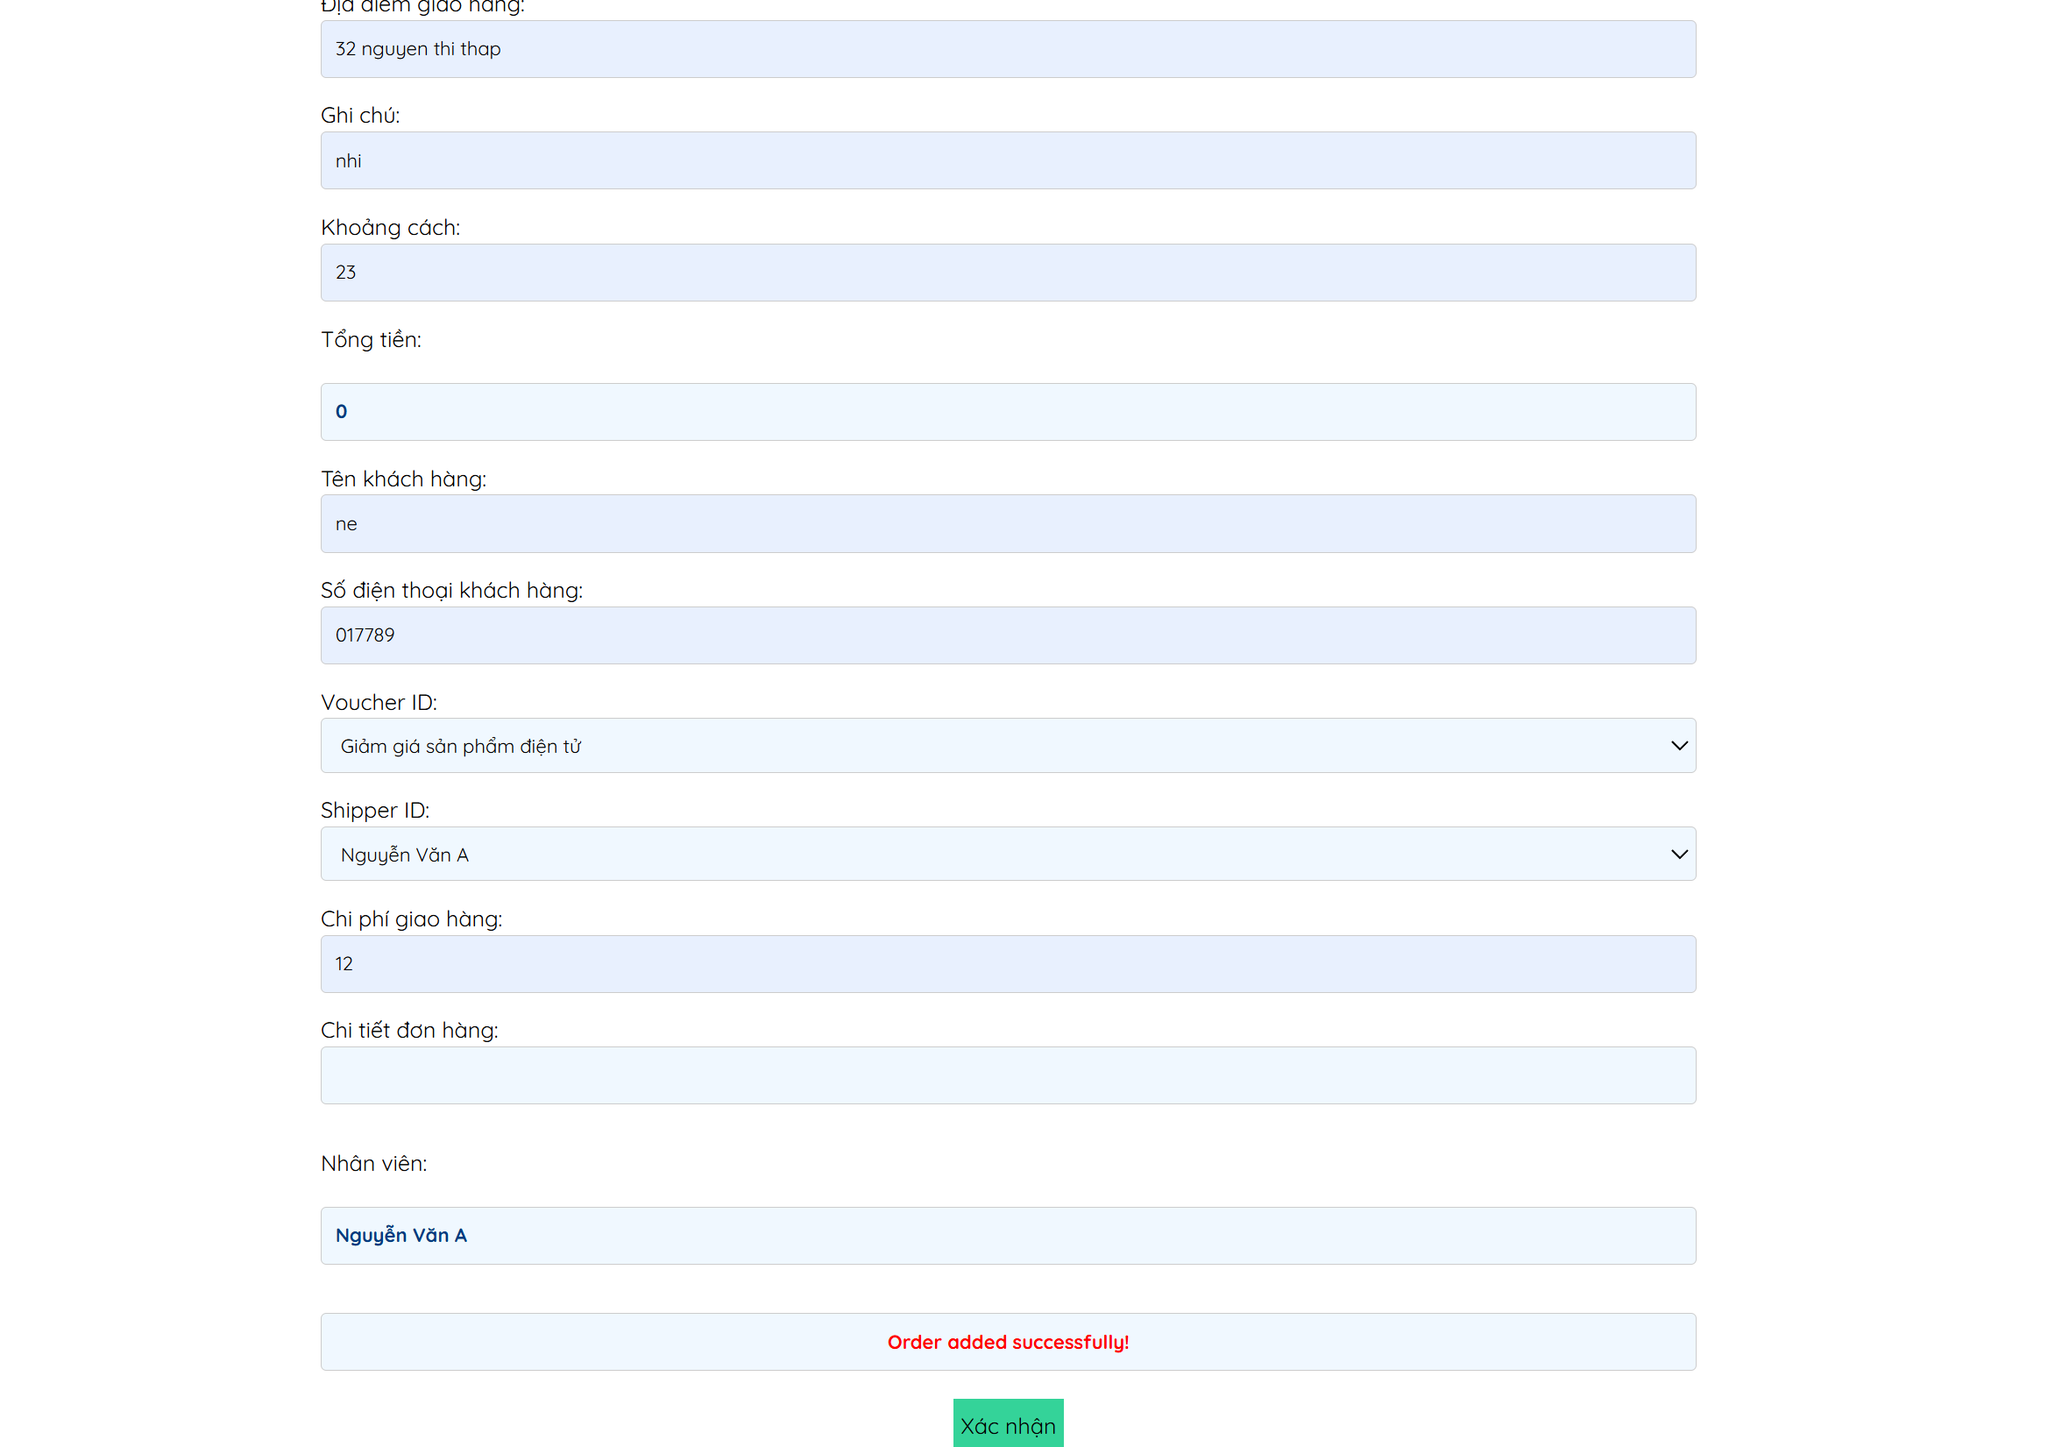
\includegraphics[scale=0.3]{Images/insertPharmaSucc.png}
        \end{figure}

        


        

\subsection{Sản phẩm}
Người dùng có thể xem thông tin chi tiết của các sản phẩm có trong kho và có thể thêm sản phẩm vào kho.
\begin{figure}[H]
\hspace*{-1cm}     
    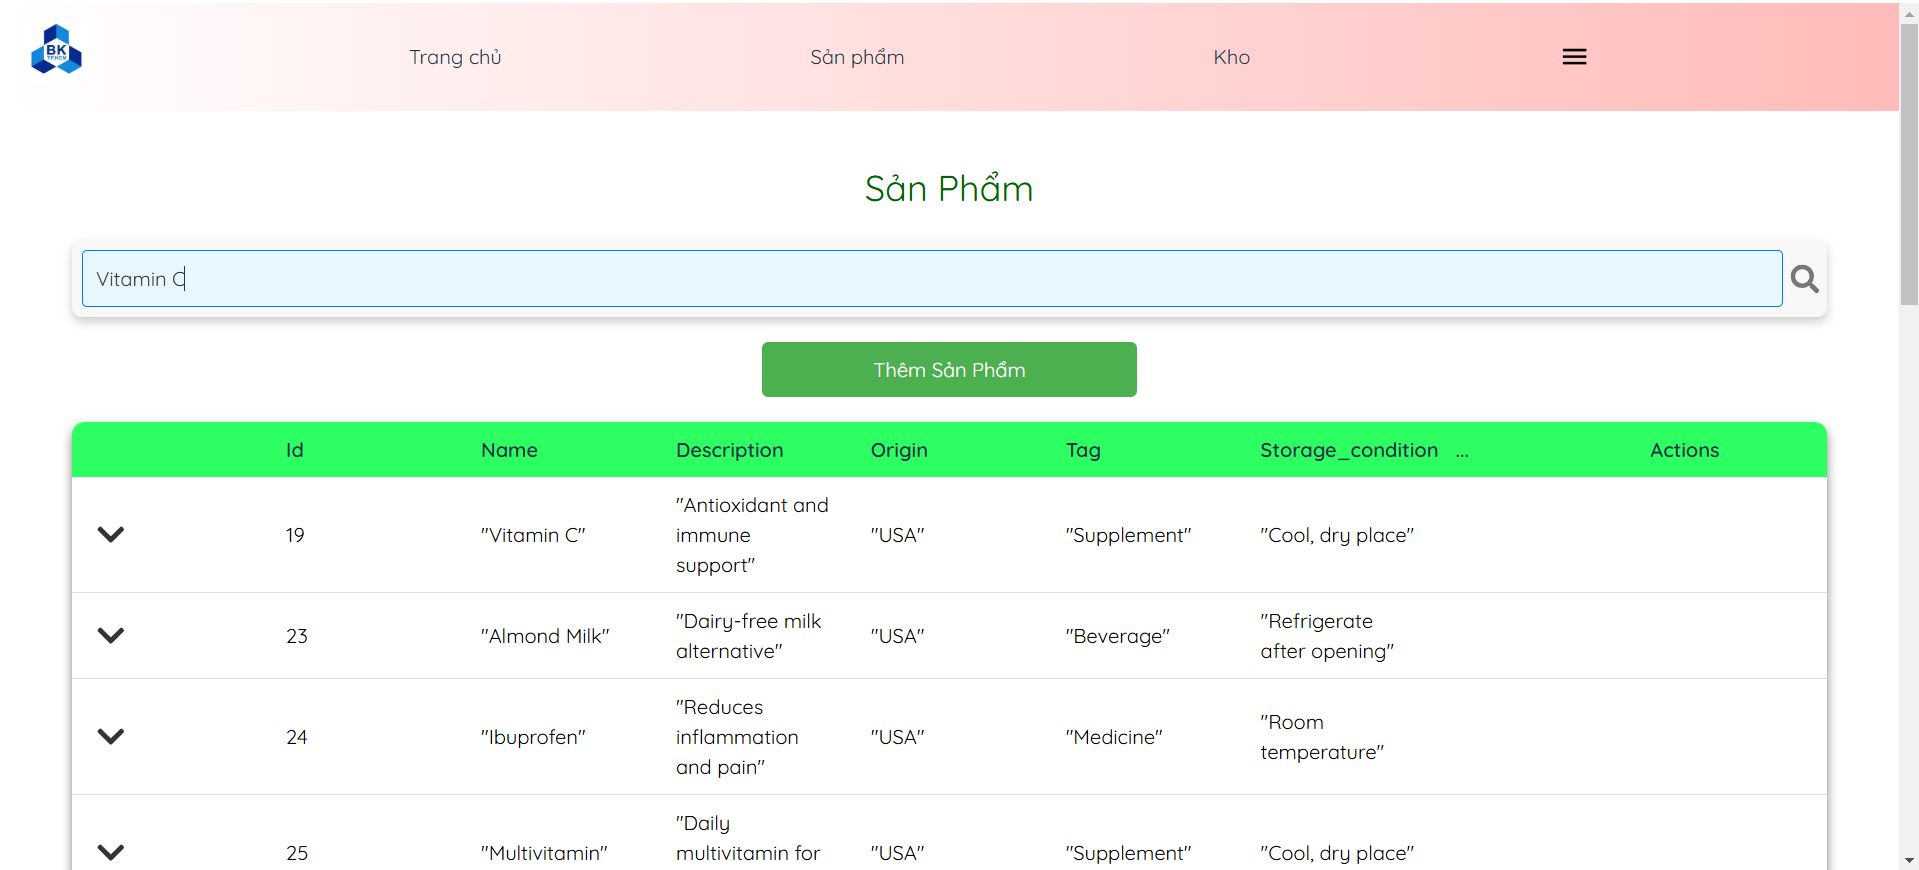
\includegraphics[scale=0.3]{Images/products_page/a1 (1).png}

\hspace*{-1cm}   
    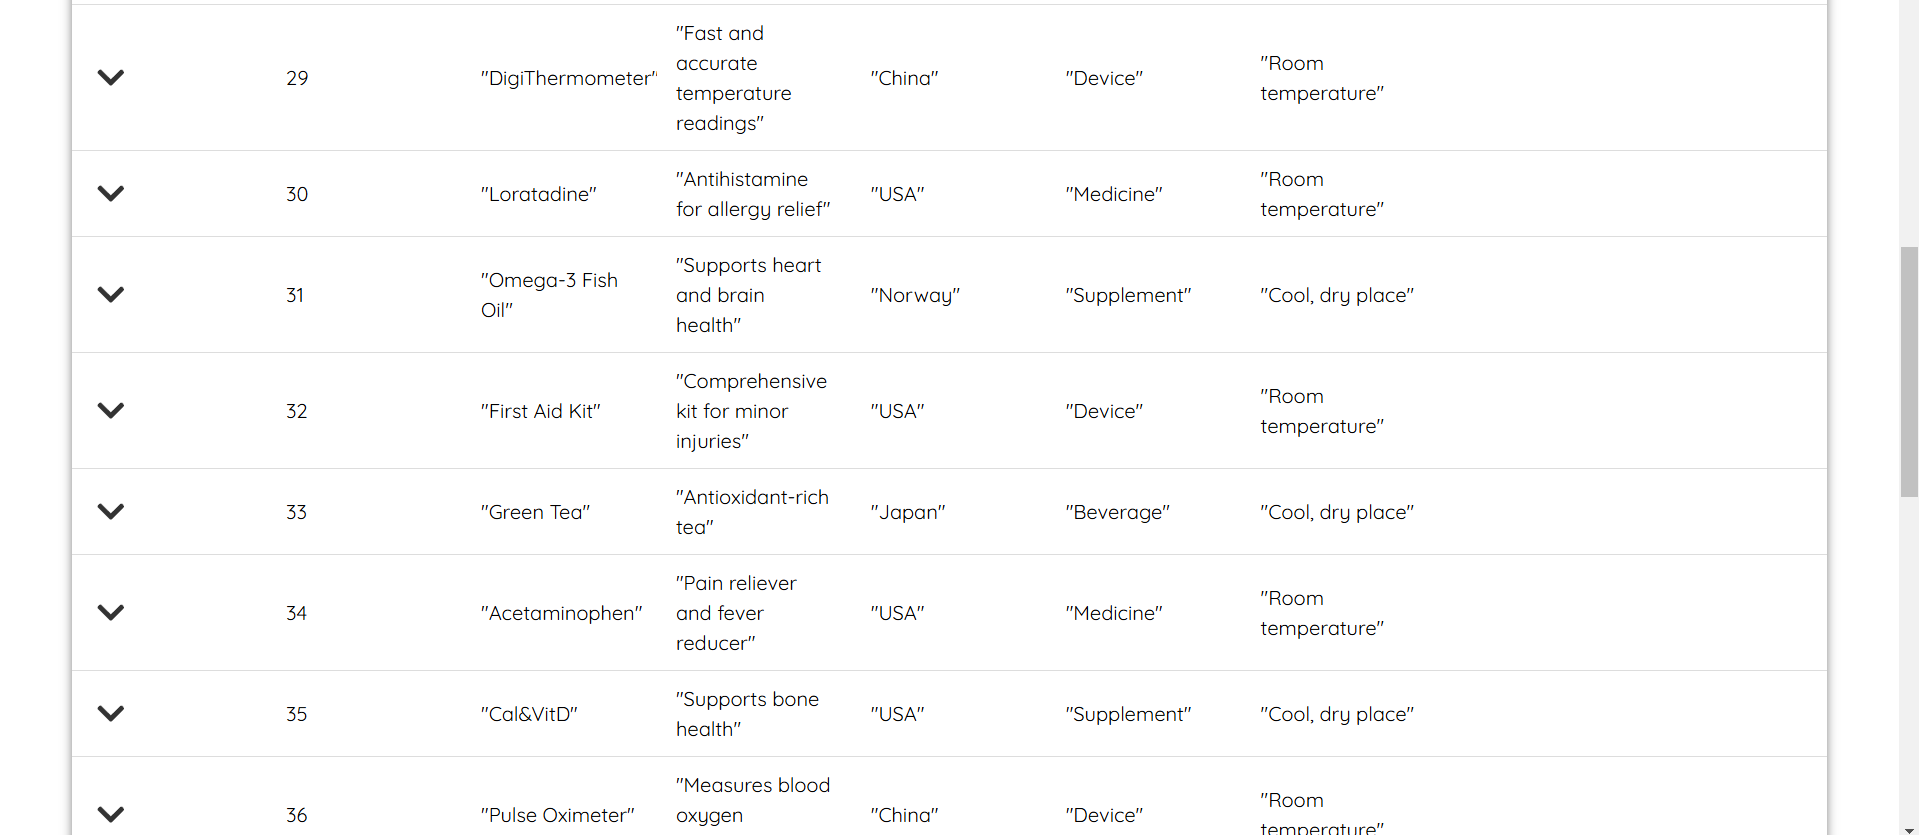
\includegraphics[scale=0.3]{Images/products_page/a1 (2).png}
\end{figure}


    \begin{figure}[H]
\hspace*{-2cm}   
%  \centering
    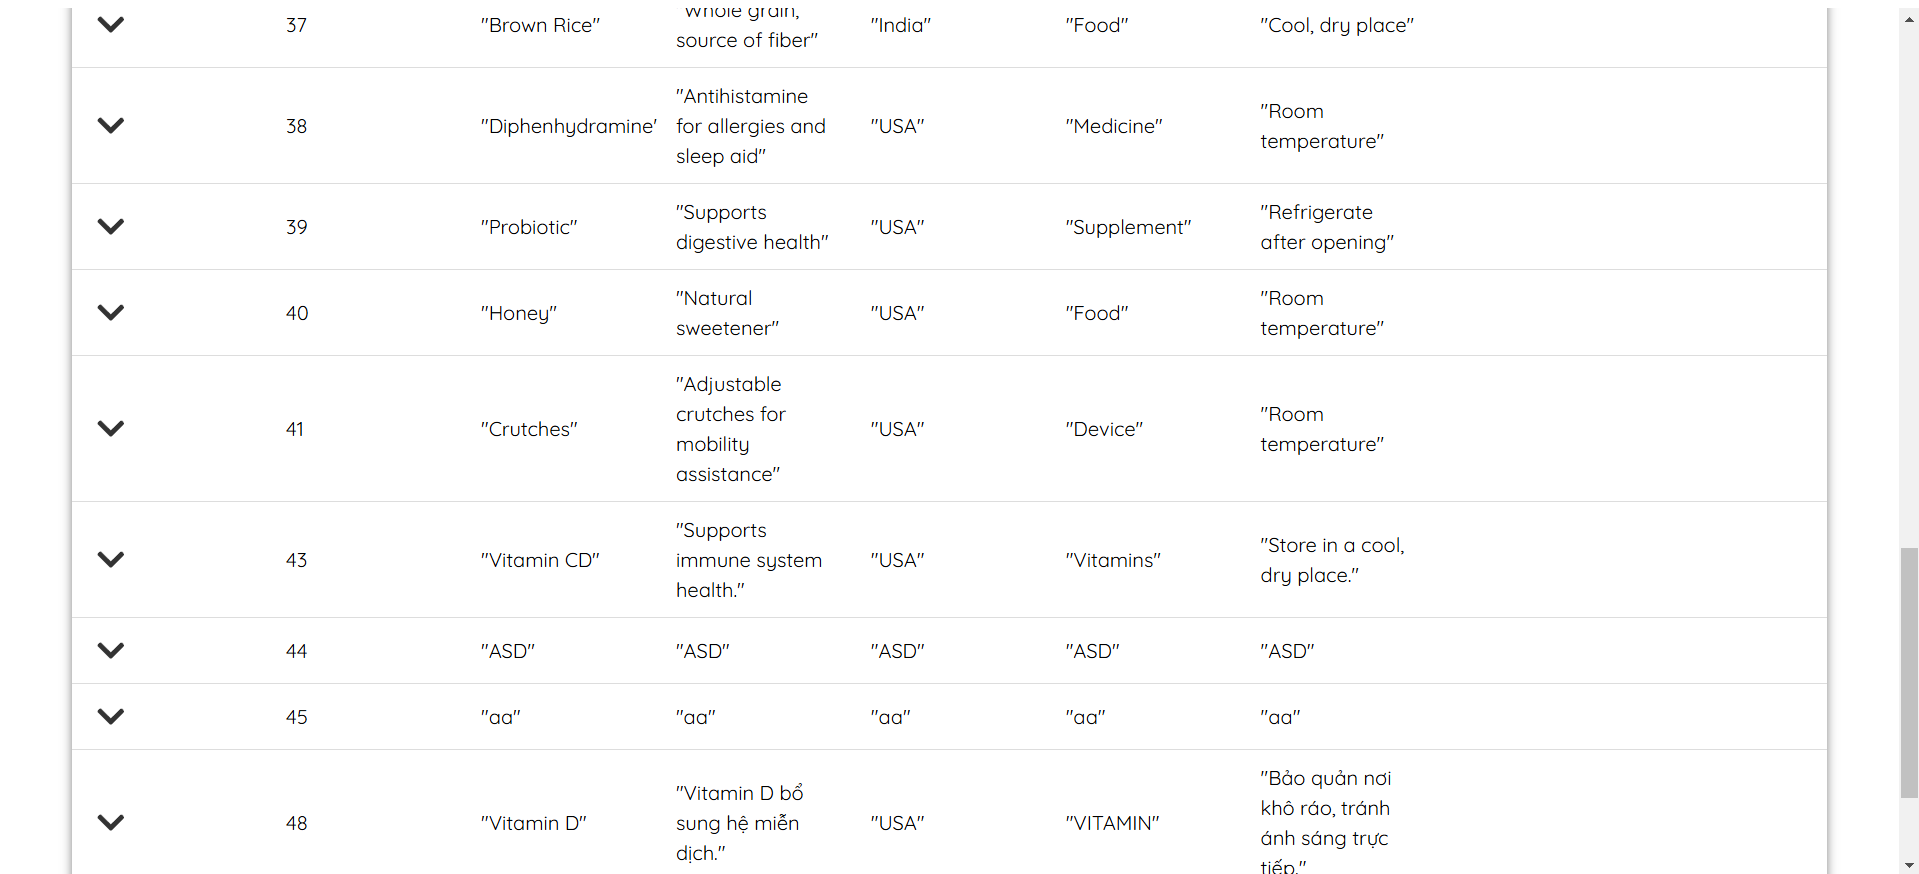
\includegraphics[scale=0.3]{Images/products_page/a1 (3).png}


\hspace*{-2cm}        
    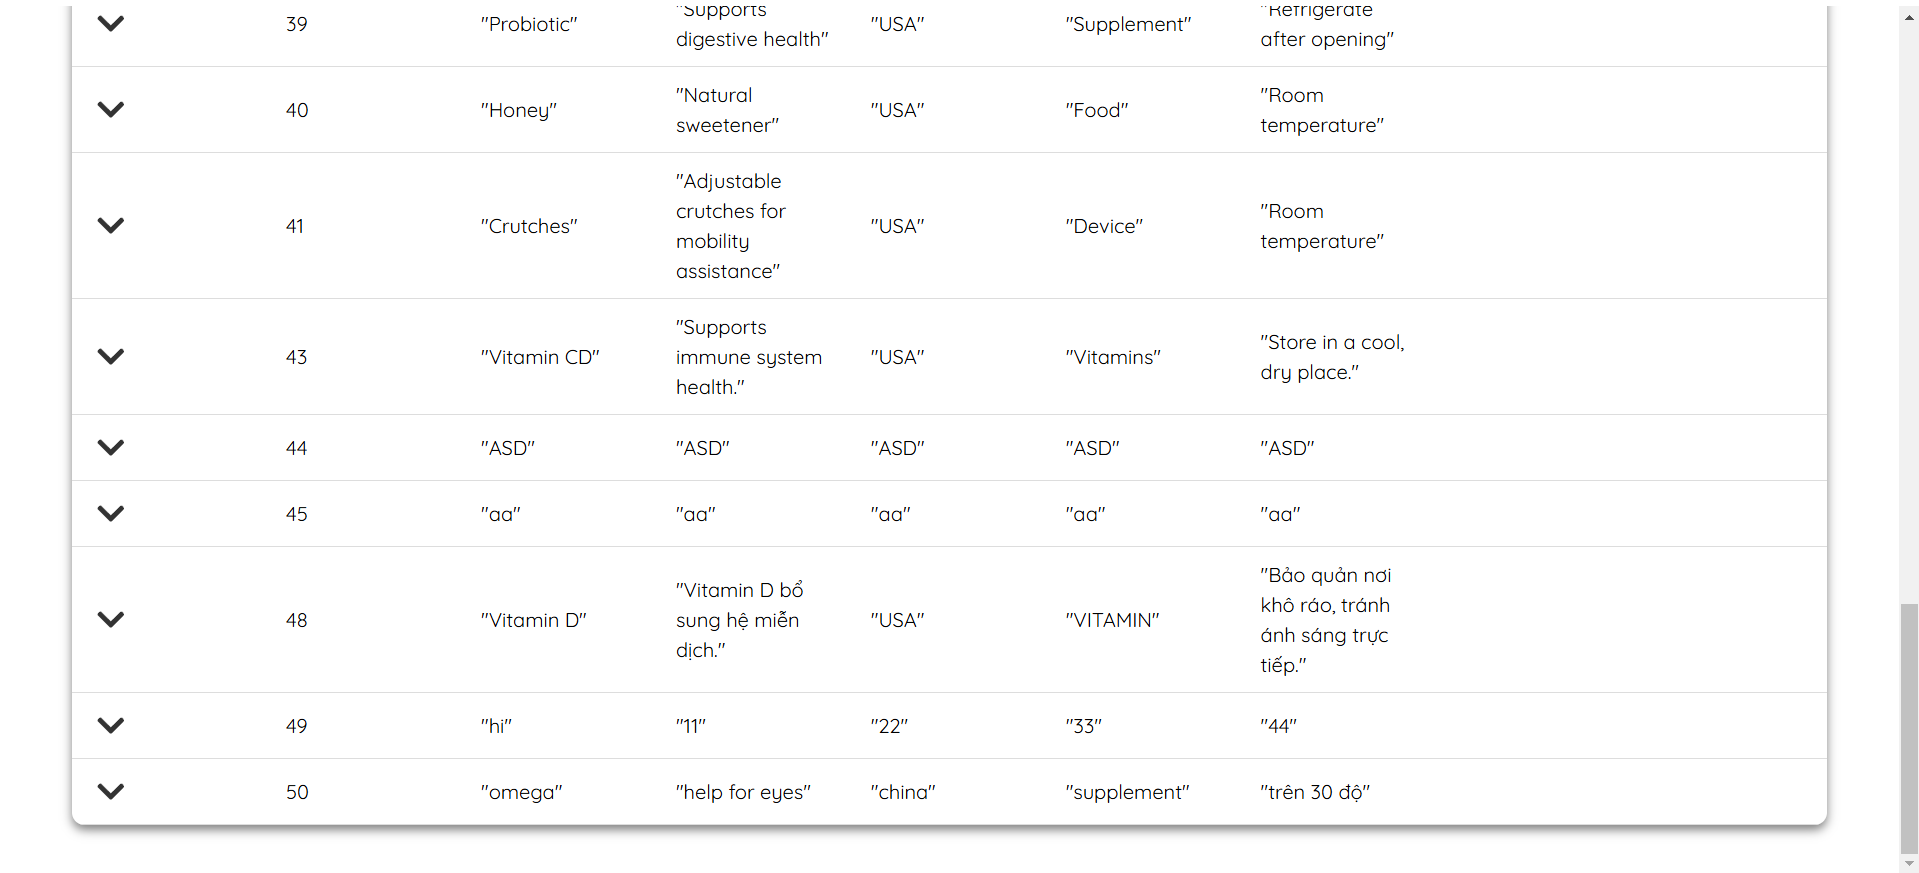
\includegraphics[scale=0.3]{Images/products_page/a1 (4).png}
    \caption{Màn hình xem các sản phẩm}
\end{figure}

\begin{figure}[H]

\hspace*{-1cm}        
    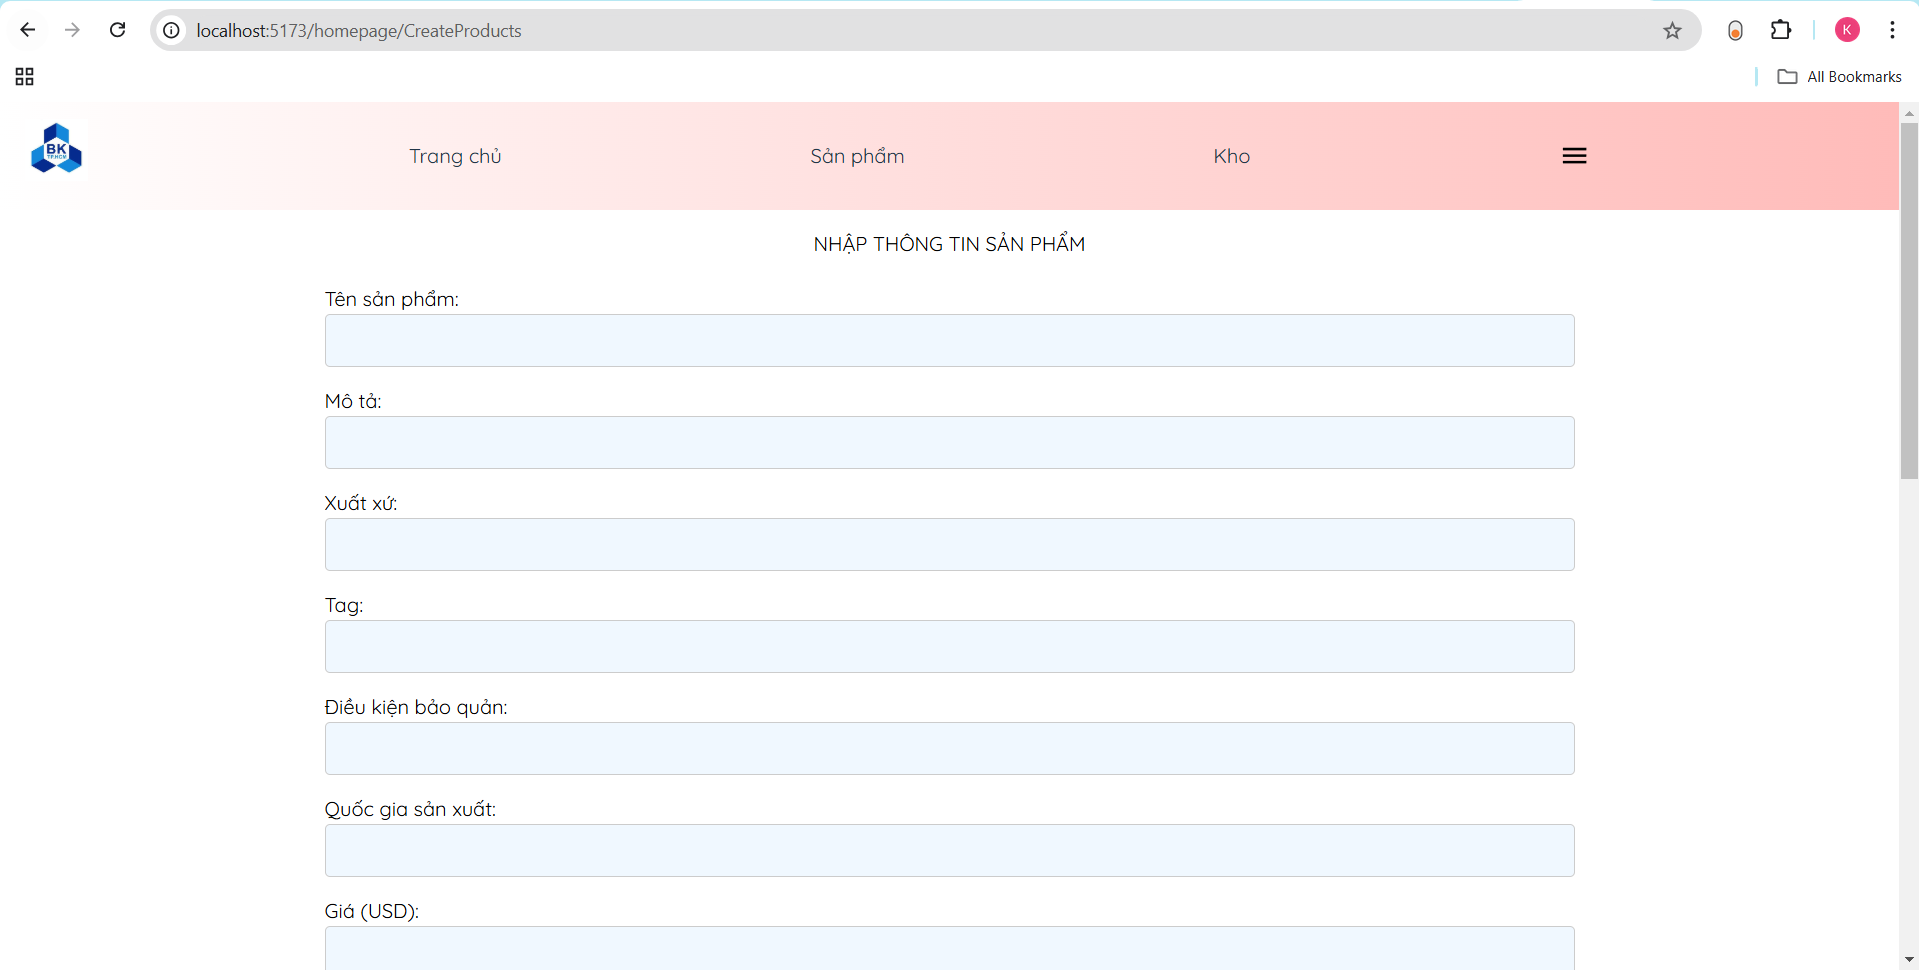
\includegraphics[scale=0.3]{Images/products_page/b1 (1).png}
    % \caption{Màn hình xem các sản phẩm}
\end{figure}

\begin{figure}[H]
\hspace*{-1cm}   
    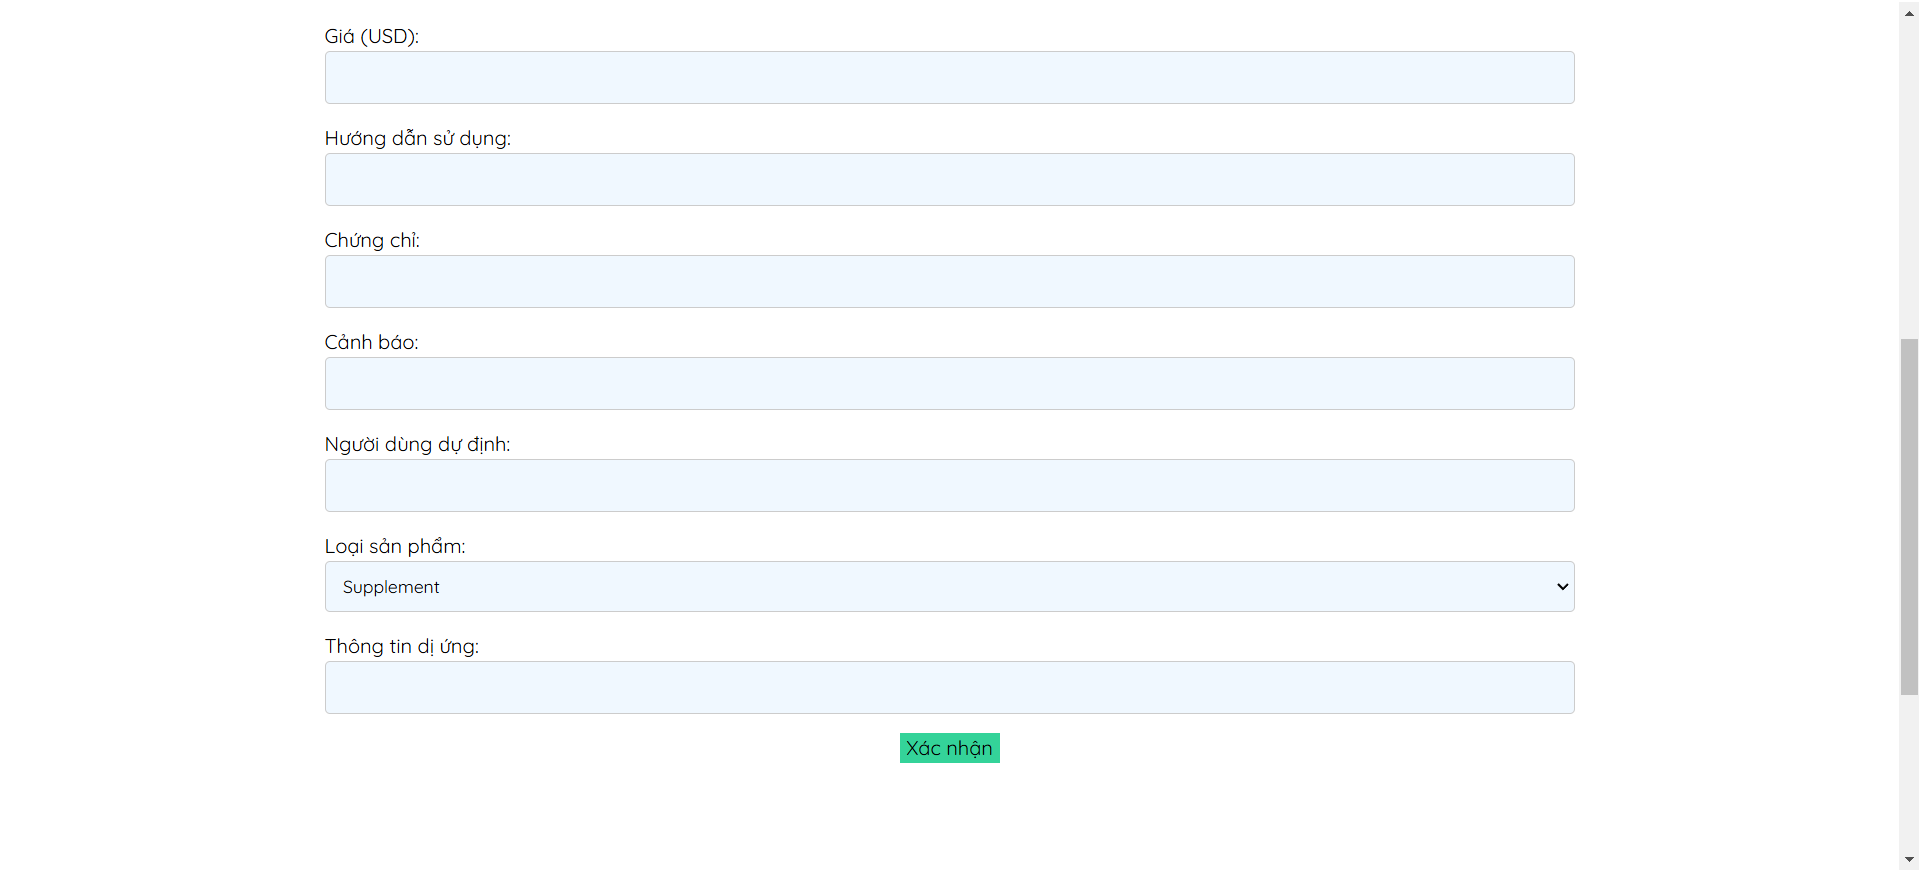
\includegraphics[scale=0.3]{Images/products_page/b1 (2).png}
    \caption{Màn hình thêm sản phẩm}
    
\end{figure}

Ngoài ra, ở phần "Thêm sản phẩm" để hạn chế người dùng nhập sai thông tin, có giới hạn độ dài của "Tên sản phẩm" và "Quốc gia sản xuất" không được quá 16 ký tự.

\begin{figure}[H]
    \hspace*{-2cm}   
        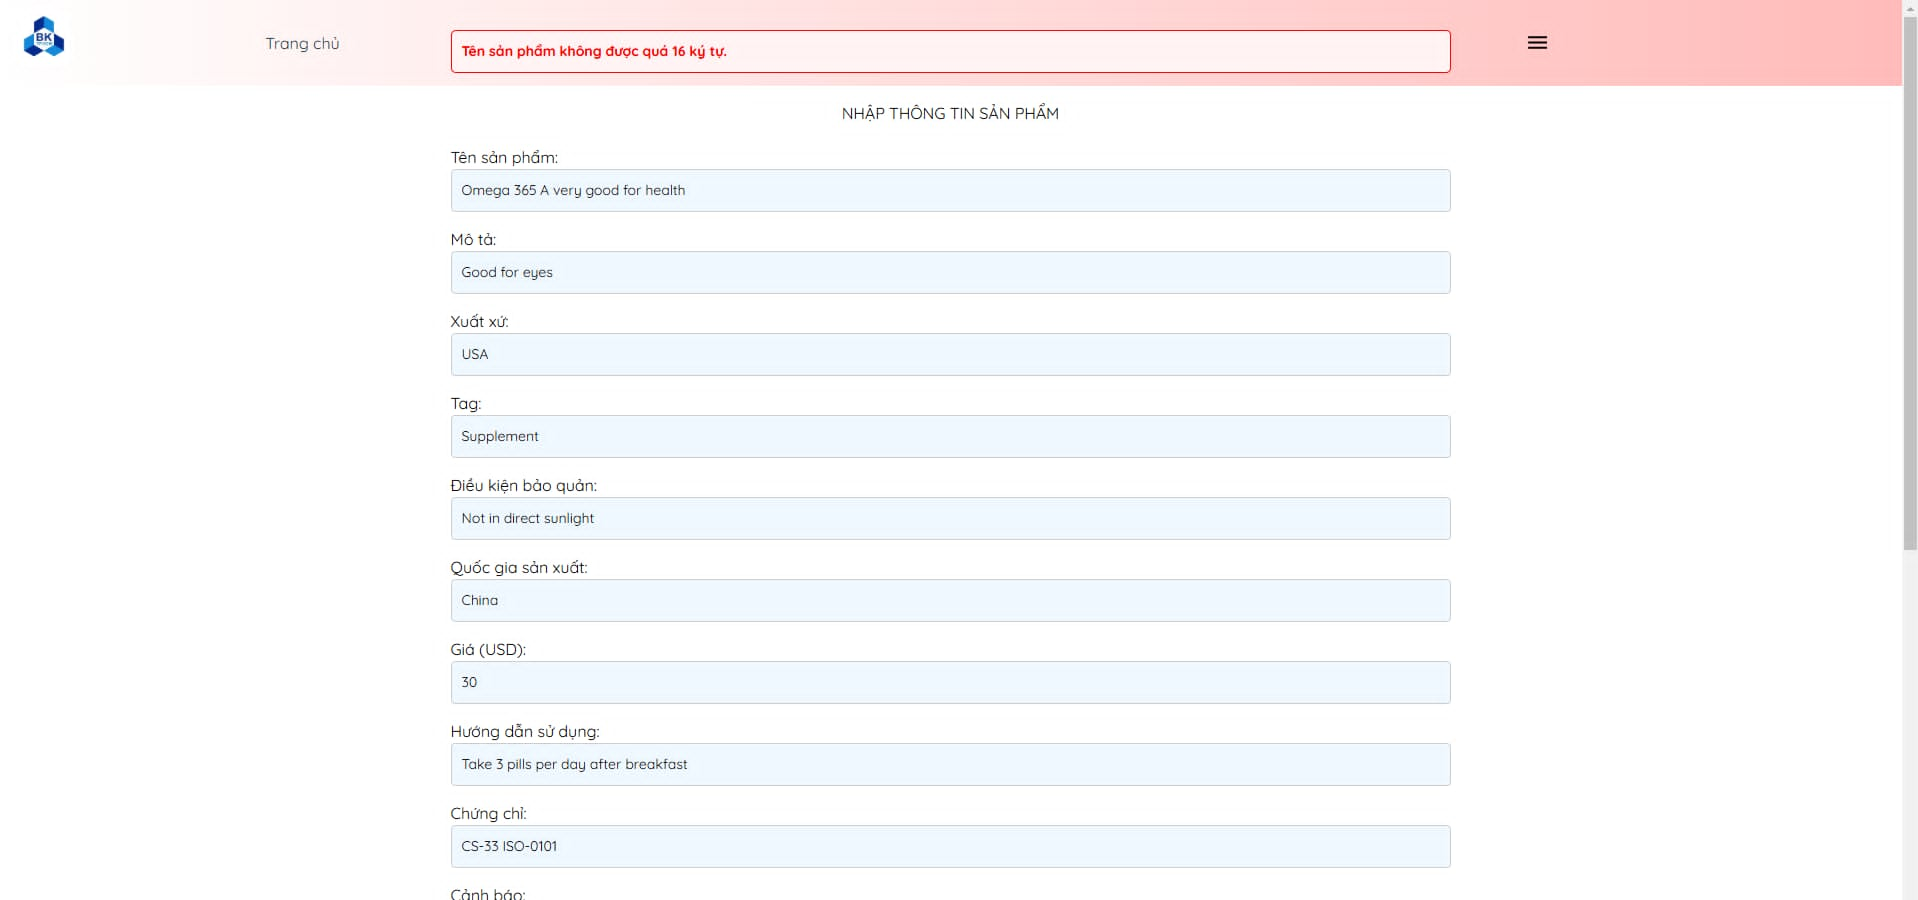
\includegraphics[scale=0.26]{Images/products_page/prod_demo_01.jpg}
    \hspace*{-2cm}   
        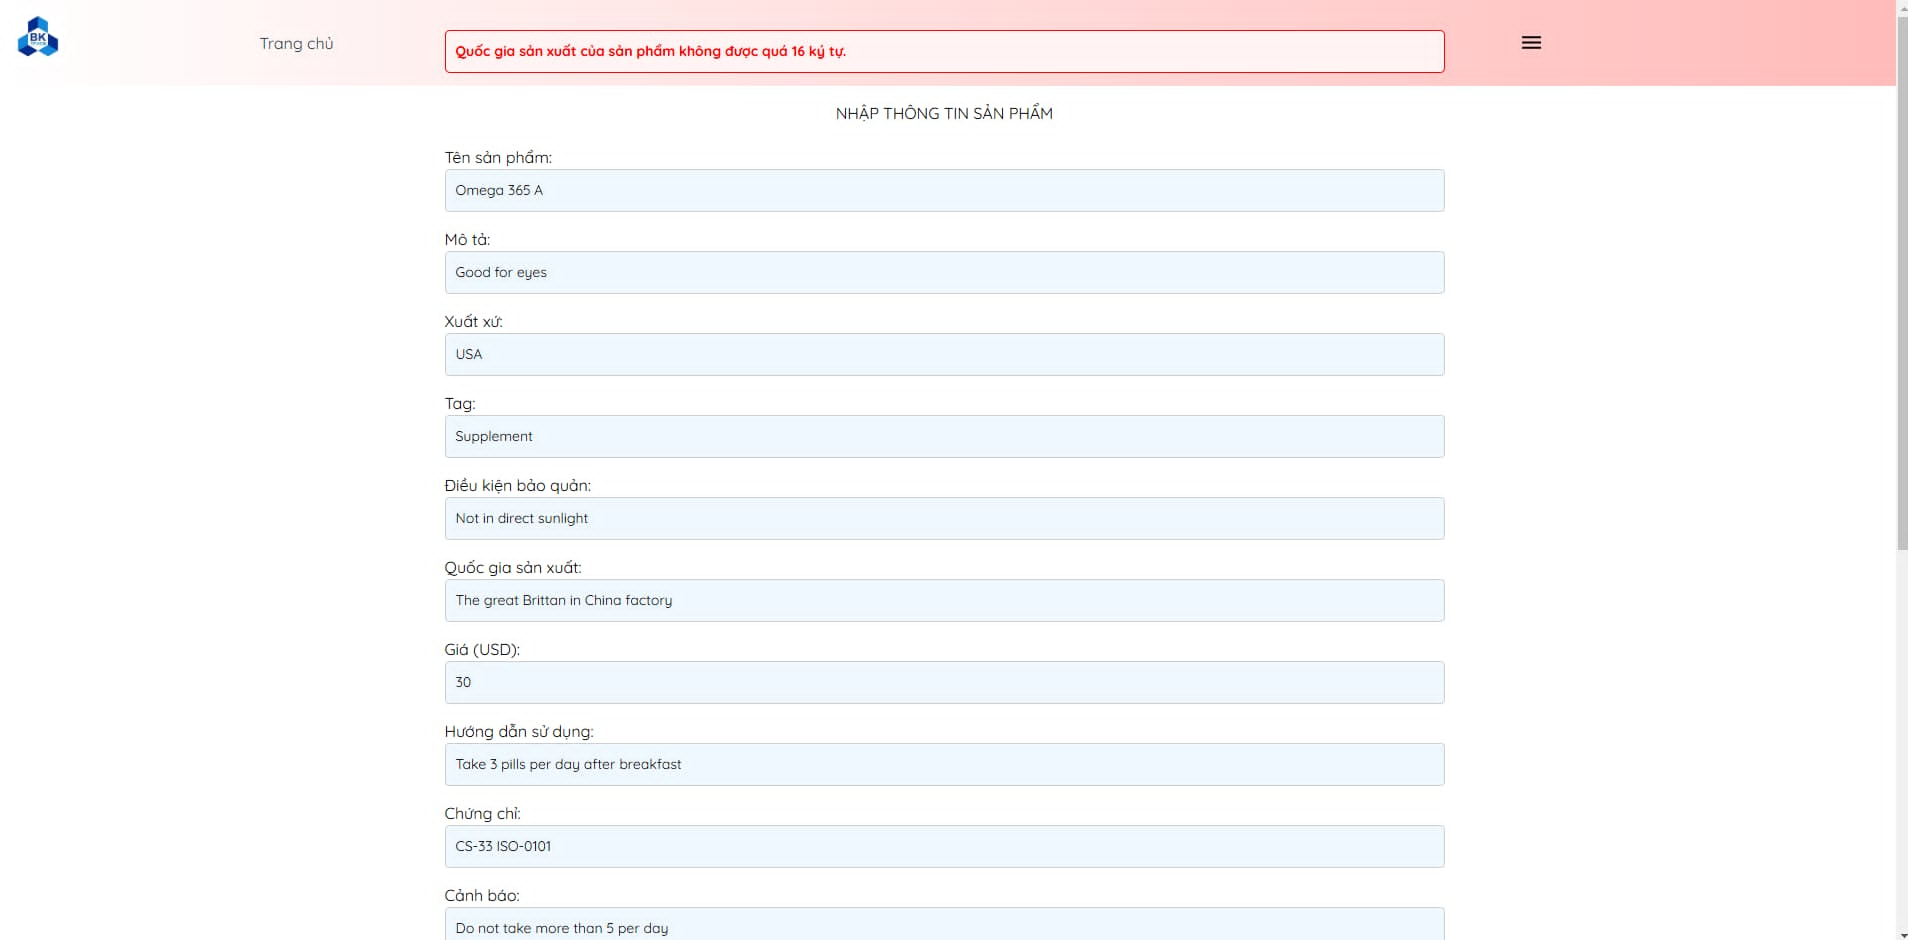
\includegraphics[scale=0.26]{Images/products_page/prod_demo_02.jpg}
        \caption{Giới hạn độ dài trong phần "Thêm sản phẩm"}
        
\end{figure}

\subsection{Kho hàng và lô hàng}
Người dùng có thể xem các lô hàng hiện có trong kho hàng và tiến hành thêm lô hàng nếu muốn.
\begin{figure}[h!]
\hspace*{-1cm}   
    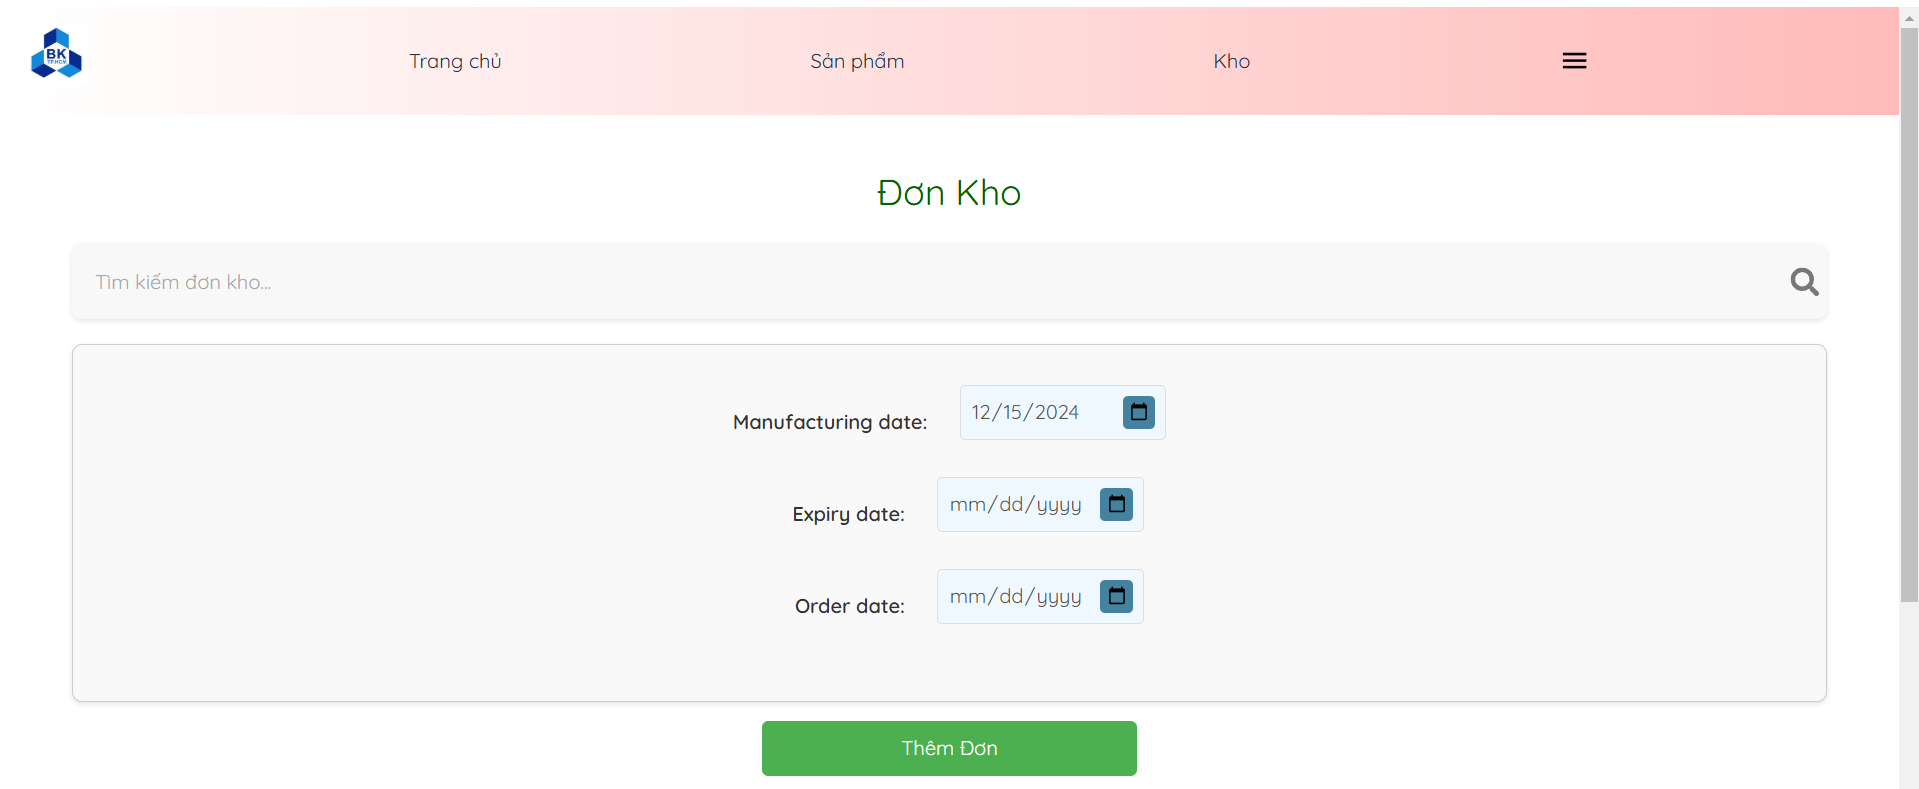
\includegraphics[scale=0.3]{Images/batch_warehouse/a2 (1).png}
    % \caption{Màn hình thêm sản phẩm}
    
\hspace*{-1cm}   
% \centering
    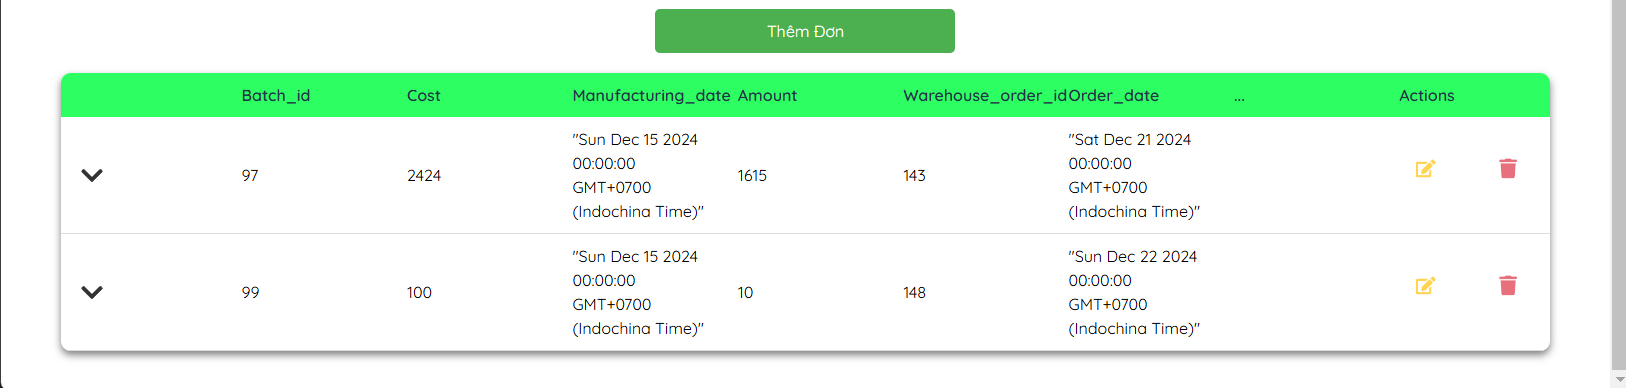
\includegraphics[scale=0.35]{Images/batch_warehouse/a2 (2).png}
    \caption{Màn hình xem thông tin lô hàng trong kho}
    
\end{figure}

\newpage

\begin{figure}[H]
\hspace*{-0.75cm}   
% \centering
    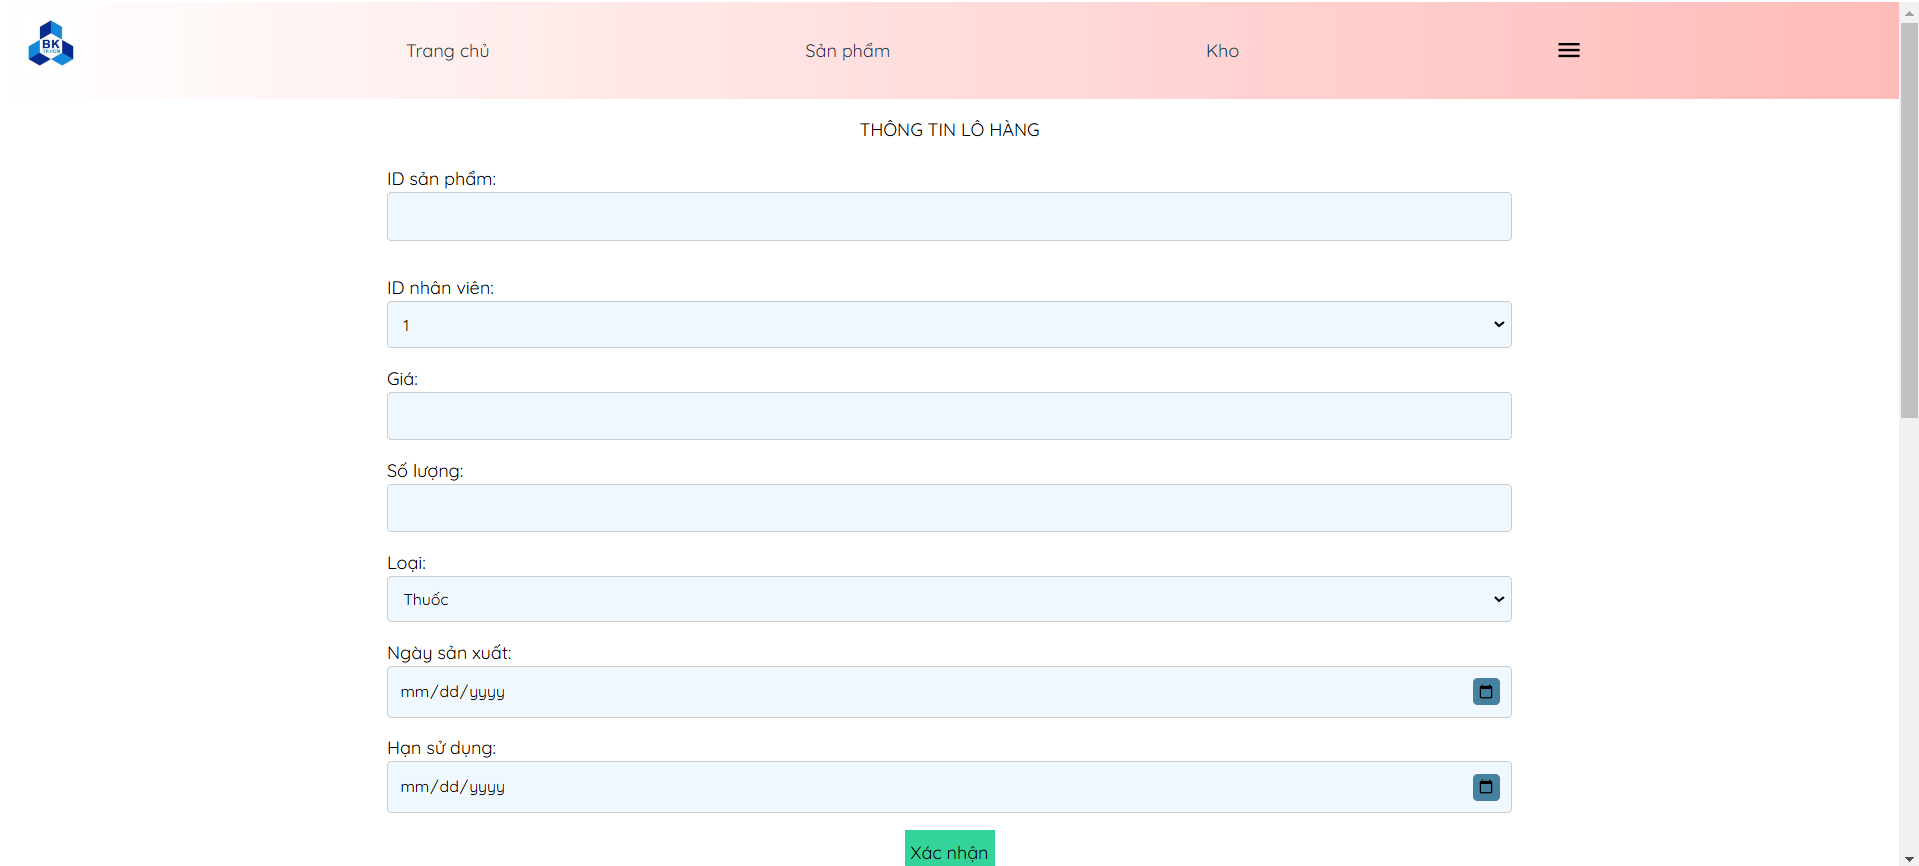
\includegraphics[scale=0.3]{Images/batch_warehouse/b3.png}
    \caption{Màn hình nhập thông tin lô}
    
\end{figure}






%%%%%%%%%%%%%%%%%%%%%%%%%%%%%%%%%


%%%%%%%%%%%%%%%%%%%%%%%%%%%%%%%%%

%%%%%%%%%%%%%%%%%%%%%%%%%%%%%%%%%

\end{document}

